
\documentclass[letterpaper,oneside]{book}%

\usepackage[left=1in,right=2.75in,top=1in,bottom=1in]{geometry}
\marginparwidth 1.75in
\usepackage{etex}
\usepackage{tabls}
\usepackage{booktabs}
\usepackage{amsmath}
\usepackage{amssymb}
\usepackage{amsthm}
\usepackage{amsfonts}
\usepackage{pstricks}
\usepackage{multicol}
\usepackage{enumitem}
\usepackage{microtype}
\usepackage{makeidx}
%\usepackage{index}
\usepackage{tikz}
\usetikzlibrary{positioning,matrix,arrows,calc}
\tikzset{every picture/.style={>=latex,thick}}
\tikzset{grid lines/.style={semithick,dotted}}

\usepackage{pgfplots} 
\pgfplotsset{compat=1.3}
\usepgfplotslibrary{external}
\tikzexternalize
\tikzsetexternalprefix{figures/}

%% comment out the following line to get color plots
\pgfplotsset{colormap/blackwhite}

\newcommand{\remake}{\tikzset{external/force remake}}

\newcommand\marginpartop[1]{\leavevmode\marginpar{#1}}

\newcommand{\aligntop}[1]{\vtop{\vskip-1ex\hbox{ #1}}}


%\newcommand{\marginpartop}[1]{\leave\marginpar{\vtop{%
%  \vskip0pt
%  \hbox{%
%    #1%
%  }}%
%}}}

\newcommand{\myscale}{1}

\usepackage{graphicx}
\usepackage{wrapfig}

\newcommand{\ds}{\displaystyle}
\newcommand{\dfdx}[1]{\frac{d#1}{dx}}
\newcommand{\ddx}{\frac{d}{dx}}

\usepackage{sagetex}


%\let\oldmarginpar\marginpar
%\renewcommand\marginpar[1]{\-\oldmarginpar{\raggedright\footnotesize #1}}
%\renewcommand\marginpar[1]{\-\oldmarginpar[\raggedleft\footnotesize #1]{\raggedright\footnotesize #1}}

\newcommand{\prepproblems}[1]{\marginpar{\fbox{\parbox{\marginparwidth}{\textbf{\raggedleft
          Target~Problems}\\ #1}}}}

\renewcommand{\thefootnote}{\roman{footnote}}
\newcommand{\note}[1]{\footnote{#1}\marginpar{\fbox{\textbf{\thefootnote}}}}
%%%%%%%To make all notes ignored, uncomment the following command.
\renewcommand{\note}[1]{}

%\usepackage[12hr]{datetime}
%\newdateformat{draftdate}{%
%\shortdayofweekname{\THEDAY}{\THEMONTH}{\THEYEAR}, %
%\THEDAY\ \shortmonthname[\THEMONTH] \THEYEAR}
%\draftdate
%\usepackage{eso-pic}
%\AddToShipoutPicture{\put(10,10){\small Draft: \today\ at \currenttime }}%--- version: \MakeUppercase{\svnInfoRevision}}}



\theoremstyle{plain}
\newtheorem{theorem}{Theorem}[chapter]
\newtheorem*{theorem*}{Theorem}
\newtheorem{lemma}[theorem]{Lemma}
\newtheorem*{lemma*}{Lemma}
\newtheorem{proposition}[theorem]{Proposition}
\newtheorem{corollary}[theorem]{Corollary}

\newtheoremstyle{box}%
{}{}% standard spacing before and after
{}% Body style
{}{\bfseries}{.}% Heading indent, font, and punctuation
{ }% space after heading
{\thmname{#1}\thmnumber{ #2}\thmnote{: #3}}% head spec


\theoremstyle{box}
\newtheorem{definition}{Definition}[chapter]
\newtheorem*{definition*}{Definition}
\newtheorem{observation}[theorem]{Observation}
\newtheorem{remark}{Remark}[chapter]
\newtheorem{example}{Example}[chapter]
\newtheorem{question}{Question}[chapter]
\newtheorem*{prep-problems}{Preparation Problems}

\newcommand{\define}[2][]{\textbf{#2}\index{#1#2}}
%\newcommand{\definemargin}[2][]{\marginpar{#2}\define[#1]{#2}}



% Abbreviations

\newcommand{\ii}{\ensuremath{\mathbf{\hat \imath}}}
\newcommand{\jj}{\ensuremath{\mathbf{\hat \jmath}}}
\newcommand{\kk}{\ensuremath{\mathbf{\hat k}}}
\newcommand{\vv}{\ensuremath{\mathbf{v}}}
\newcommand{\colvec}[1]{\ensuremath{\begin{bmatrix}#1\end{bmatrix}}}
\DeclareMathOperator{\rank}{rank}
\DeclareMathOperator{\rref}{rref}
\DeclareMathOperator{\vspan}{span}
\DeclareMathOperator{\trace}{tr}
\DeclareMathOperator{\proj}{proj}
\DeclareMathOperator{\curl}{curl}
\newcommand{\RR}{\ensuremath{\mathbb{R}}}
% \vp is "vector prime" and corrects spacing when doing something like
% $\vec r'$ (which has the vector and prime almost touching).
% Instead, do something like $\vec r\vp$
\newcommand{\vp}{\ensuremath{^{\,\prime}}}

%The purpose of this code is to allow me to put lines in matrices so that I can create augmented matrices.
\makeatletter
\renewcommand*\env@matrix[1][*\c@MaxMatrixCols c]{%
  \hskip -\arraycolsep
  \let\@ifnextchar\new@ifnextchar
  \array{#1}}
\makeatother

\newcommand{\cl}[1]{  \begin{matrix}  #1  \end{matrix}  }
\newcommand{\bm}[1]{  \begin{bmatrix}  #1  \end{bmatrix}  }
\newcommand{\inv}{^{-1}}
\newcommand{\im}{\ensuremath{\text{im }}}
\newcommand{\R}{\mathbb{R}}
\providecommand{\norm}[1]{\lVert#1\rVert} 


%------------------------------------------------------------------------------------------------------------

\usepackage{hyperref}
%\makeindex

\begin{document}
\newgeometry{left=1in,right=1in,top=1in,bottom=1in}

\frontmatter
\title{Multivariable Calculus}
\author{Ben Woodruff\thanks{Mathematics Faculty at Brigham Young
    University--Idaho, \url{woodruffb@byui.edu}} \and Jason
  Grout\thanks{\mbox{Mathematics Faculty at Drake University, Des Moines,
    IA, \url{jason.grout@drake.edu}}}}
\date{Typeset on \today\\
\vfill

\includegraphics[height=1.3cm]{by-sa}
\vfill}
\maketitle
\thispagestyle{empty}

\noindent\copyright{ 2010 Ben Woodruff and Jason Grout.  Some Rights Reserved.\\

\bigskip

\noindent Except where otherwise noted, this work is licensed under the Creative Commons
Attribution-ShareAlike 3.0 United States License. To view a copy of
this license, visit 
\begin{center}
  \url{http://creativecommons.org/licenses/by-sa/3.0/us/}
\end{center}
or send a letter to Creative Commons, 171 Second Street, Suite 300,
San Francisco, California, 94105, USA.

\bigskip

\noindent Please attribute this work to:
\smallskip

Ben Woodruff, Mathematics Faculty at Brigham Young University--Idaho,
 \url{woodruffb@byui.edu}, and

\smallskip

 Jason Grout, Mathematics Faculty at Drake University, Des Moines, IA,
 \url{jason.grout@drake.edu}.

\vfill 

The source for this work is available at \url{http://github.com/jasongrout/multivariable-calculus}.
\vfill
}
\restoregeometry
\tableofcontents



%\chapter*{Preface}
%
%I would like to thank BYU-Idaho for the resources they have provided me to create this text.  

%\chapter{Introduction}
%
%The introduction is entered using the usual chapter command. Since
%the introduction chapter appears before the \verb|mainmatter| TeX
%field, it is again an unnumbered chapter. The primary difference
%between the preface and the introduction in this sample document
%is that the introduction will appear in the table of contents and
%the page headings for the introduction are automatically handled
%without the need for the \verb|markboth| TeX field. You may use
%either or both methods to create chapters at the beginning of your
%document. You may also delete these preliminary chapters.





\mainmatter


\chapter{Curves, Coordinates, and Differentials}

This chapter covers the following ideas. 


\begin{enumerate}

\item Model motion in the plane using parametric equations. In particular, how do you describe circles, ellipses, and lines using parametric equations.
\item Be able to convert between rectangular and polar coordinates. 
\item Graph polar functions in the plane. Find intersections of polar equations, and illustrate that not every intersection can be obtained algebraically (you may have to graph the curves).
\item Find derivatives, tangent lines, area, arc length, and surface area using parametric and polar equations.

\end{enumerate}


%%% Local Variables: 
%%% mode: latex
%%% TeX-master: "../multivariable-calculus"
%%% End: 




\section{Parametric Equations}

How can we describe motion in the plane?  One idea is to let $t$ represent time, and then write two equations $x=f(t),y=g(t)$ to describe the $(x,y)$ location of the point at any time $t$.  This gives us our first example of a mathematical ``function'' where we put in one value $t$ and get out two values $x$ and $y$.  This approach gives us a valuable way to study motion in the plane. The equations $x(t), y(t)$ are called parametric equations of a curve.

The parametric equations $x = \cos t, y=\sin t$ for $0\leq t\leq 2\pi$ describe motion along a circle of radius 1 in the plane.  You can convince yourself of this by plotting the points for various values of $t$ (make a $t,x,y$ table and start plotting points).  Alternatively, if you recall that $\cos^2 t+\sin^2 t = 1$, then you can replace $\cos t$ with $x$ and $\sin t$ with $y$ to obtain $x^2+y^2=1$, a Cartesian equation for a circle of radius 1.  Similarly you can show that $x=a\cos t, y=b\sin t$ for $0\leq t\leq 2\pi$ gives equations for an ellipse of the form $\frac{x^2}{a^2}+\frac{y^2}{b^2}=1$.  The graph of a function of the form $y=f(x)$ can always be written parametrically as $x=t,y=f(t)$, and then any equation we studied in first semester calculus can be analyzed using parametric equations. Using the identity $\cosh^2 x-\sinh^2 x =1$, the parametric equations $x=\cosh t,y=\sinh t$ give parametric equations for a hyperbola $x^2-y^2=1$, where $-\infty<t<\infty$. Because $\cosh x$ and $\sinh x$ trace out a hyperbola as parametric equations, they are called the hyperbolic trigonometric functions.  

To parametrize the line segment from $(1,2)$ to $(2,3)$, let's start by giving a Cartesian equation. The slope is $1/2$, so an equation is $y-2=\frac{1}{2}(x-1)$.  One option is to let $x=t$ and then $y=2+\frac{1}{2}(t-1)$. In this case, to get the curve to start at $x=1$ and end at $x=2$, we require $1\leq t\leq 2$. Another option is to let $t=\frac{1}{2}(x-1)$ or $x=1+2t$, and then $y-2=t$ or $y=2+t$. When $x=1$ we have $t=0$, and when $x=2$ we have $t=1/2$, so we require $0\leq t\leq 1/2$. There are infinitely many ways to parametrize the same curve.

We need to learn how to write parametric equations given a curve, and we need to learn how to find a Cartesian equation (remove $t$ from the equations) when we are given parametric equations.  In the textbook in 10.2, they give an example of the cycloid which leads to parametric equations. It is not crucial that you master the ideas behind a cycloid, rather that you learn how to parametrize curves. We will practice this idea in class all semester long. Obtaining a skill in parameterizing curves requires lots of practice. 

\subsection{Derivatives and Tangent lines}
How do you find the slope $\frac{dy}{dx}$ for a parametric curve?  The simple answer comes from the chain rule and essentially can be thought of as divide the top and bottom by $dt$, giving $\frac{dy}{dx} = \frac{dy/dt}{dx/dt}$. In other words, the derivative with respect to $x$ is found by dividing derivatives with respect to $t$.  This allows us to find tangent lines and more.  To find the second derivative $\frac{d^2y}{dx^2}$, we first find $dy/dx$ and then compute $d(dy/dx)/dt$ and divide it by $dx/dt$, namely 
$\ds \frac{d(\frac{dy}{dx})}{dx} = \frac{d(\frac{dy}{dx})/dt}{dx/dt}$ 
(again divide the top and bottom by $dt$). Often times people use dots to denote derivatives with respect to $t$, so we could write this as $dy/dx=\dot y/\dot x$.

As an example, consider the ellipse $x=\cos t, y=\sin t$. The derivatives with respect to $t$ are $\dot x = dx/dt = -\sin t$ and $\dot y= dy/dt=\cos t$. The derivative of $y$ with respect to $x$ is $dy/dx = \dot y/\dot x = \frac{\cos t}{-\sin t} = -\cot t$.  The derivative of $y'$ with respect to $t$ is $(-\cot t)' = \csc^2 t$. Dividing this by $\dot x = -\sin t$ gives $d^2y/dx^2 = \csc^3t$.  To find the tangent line to the curve at $t=\pi$, we compute  $x=\sqrt 2/2, y=\sqrt 2/2$, and $dy/dx = -\cot (\pi/4) = -1$. Using the point-slope form of a line, we have the tangent line as $(y-\sqrt 2/2) = -1 (x-\sqrt 2 /2)$.



\section{Polar Coordinates}

We now introduce a new coordinate system, the polar coordinate system.  This is just another way of referencing points in the plane.  We use {$r$ and {$\theta$ to reference points.  The distance from the origin to the point {$P$ is called {$r$, and the angle made by the positive {$ x $-axis and a ray from the origin through {$ P $ is called {$ \theta $.  The key equations $ x=r\cos\theta, y=r\sin\theta , x^2+y^2=r^2$ come directly from a right triangle with one vertex at the origin, another at the point $P$, and another directly above or below $P$ on the $x$-axis. 

The point $(r,\theta) =(2, \pi/2)$ represents the point $(x,y)=(0,2)$. The point $(r,\theta) =(3, \pi/4)$ represents the point $(x,y)=(3\frac{\sqrt{2}}{2},3\frac{\sqrt{2}}{2})$. Notice that the point $(1,\pi)$ in polar coordinates is the same as the point $(1,3\pi)$ or $(-1,-\pi)$ in polar coordinates.  The same $(x,y)$ point in the plane can be represented by infinitely many different polar coordinate pairs.
\subsection{Converting between polar and Cartesian coordinates and graphing}
The graph of $r=2$ is a circle of radius $2$ in the plane.  The graph of $\theta =  \pi/3$ is a straight line through the origin with angle of inclination $\pi/3$.  The line $x=4$ can be rewritten in polar coordinates as $r\cos\theta = 4$, or $r=4\sec\theta$.  The polar coordinate equation $r=2\sin\theta $ can be converted to rectangular coordinates by multiplying both sides by $r$, giving $r^2 = 2r\sin\theta$, and then using the key equations to obtain $x^2+y^2 = 2y$, which is the equation of a circle $x^2+y^2-2y+1=1$, or $x^2+(y-1)^2=1$ centered at $(0,1)$ of radius $1$ (I completed the square to complete this example). The key equations will allow you to convert from one system to another. You may need to multiply both sides of an equation by $r$ to do a conversion (as in the last example).

To plot a polar equation, we just make an $r,\theta, x,y$ table and start plotting points.  You will discover after some practice that there are symmetries that you can use to help you learn how to plot polar curves.  To plot the curves by hand, try putting in values of $\theta$ which are on the unit circle, in particular use $0,\pi/2,\pi,3\pi/2$.  When you connect dots on your graphs, realize that you wrap around counter-clockwise as theta increases, and the variable $r$ that is changing is the distance from the origin.  Some common curves are shown below:

\newcommand{\mywidth}{1.3in}
\begin{center}
\begin{tabular}{cccc}
%polar_plot(cos(3*x),(x,0,2*pi),color='black',aspect_ratio=1).save('rose.pdf',aspect_ratio=1)
%polar_plot(2*cos(x)+1,(x,0,2*pi),color='black',aspect_ratio=1).save('limacon.pdf',aspect_ratio=1)
%polar_plot(1-cos(x),(x,0,2*pi),color='black',aspect_ratio=1).save('cardioid.pdf',aspect_ratio=1)

% cosines = [cos(-pi/2+pi*i/100) for i in range(201)]
% v = [(1/c, tan(-pi/2+pi*i/100)) for i,c in enumerate(cosines) if c != 0]
% L = [(a/(a^2+b^2), b/(a^2+b^2)) for a,b in v]
% p = line(L, color='black')
% p.save('lemniscate.pdf',aspect_ratio=1)

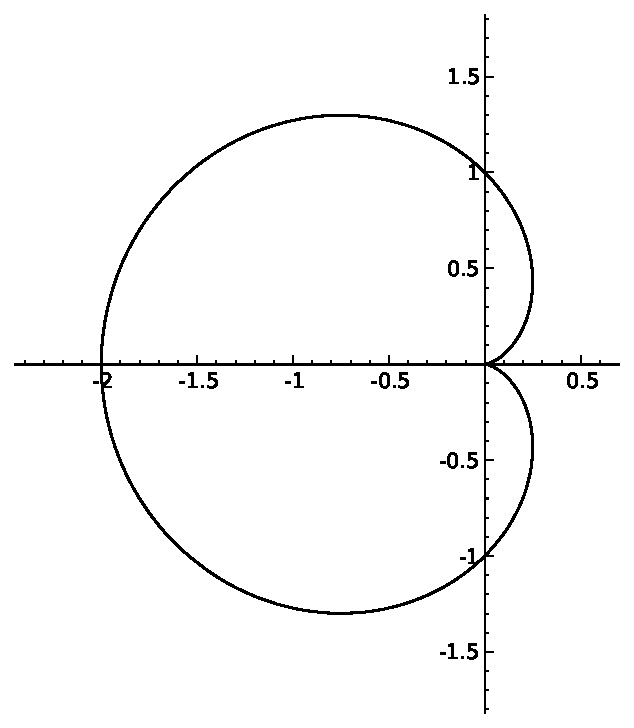
\includegraphics[width=\mywidth]{01-Curves-Coordinates-Differentials/cardioid}&
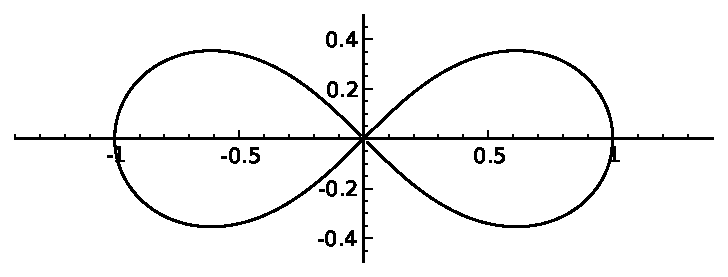
\includegraphics[width=\mywidth]{01-Curves-Coordinates-Differentials/lemniscate}&
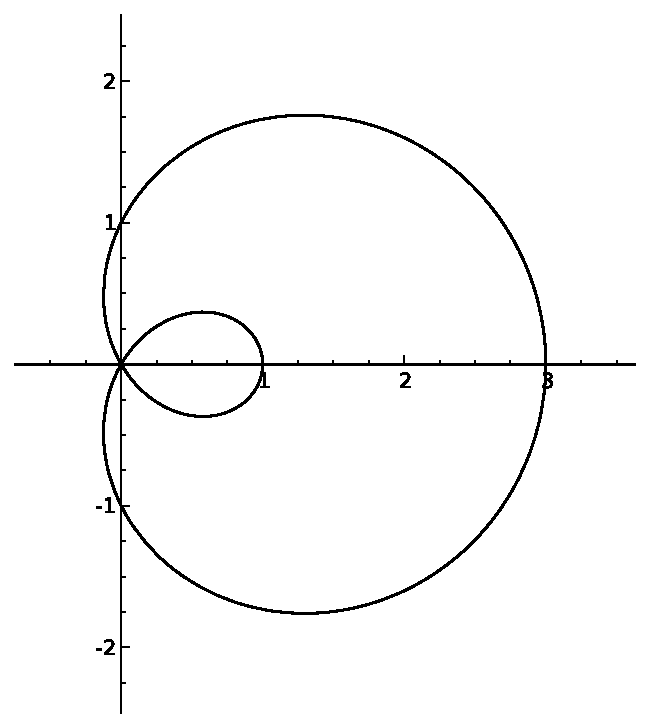
\includegraphics[width=\mywidth]{01-Curves-Coordinates-Differentials/limacon}&
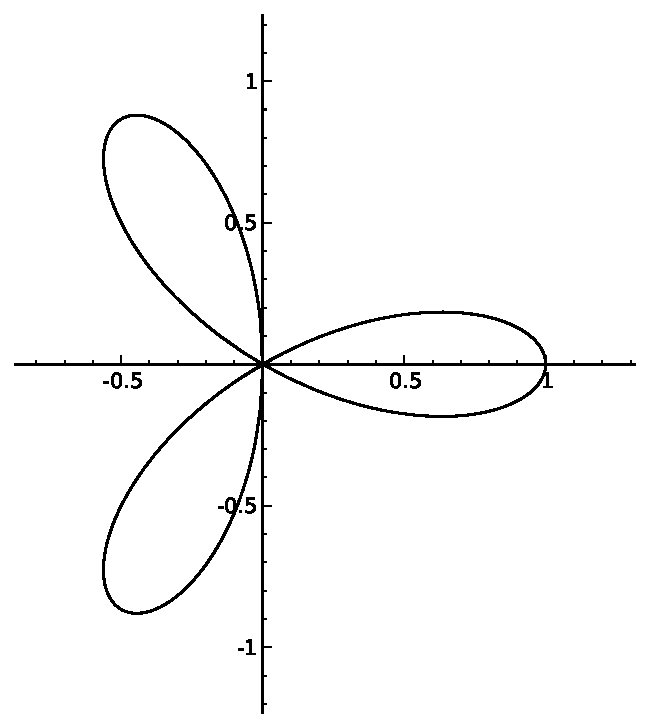
\includegraphics[width=\mywidth]{01-Curves-Coordinates-Differentials/rose}
\\
Cardioid&
Lemniscate&
Limacon&
Rose
\\
$r=1-\cos\theta$&
$r^2=\sin 2\theta$&
$r=2\cos\theta+1$&
$r=\cos 3\theta$
\end{tabular}
\end{center}

\subsection{Finding Intersections}
One problem with finding the intersection of two polar graphs is that there are many ways to represent the same point in polar coordinates.  Hence, when you solve for the intersection of two polar graphs, you may not find all the intersection points algebraically. Often you must graph the polar curves in addition to finding the points of intersection.  For example, the two curves $r=1-\cos\theta$ (a cardioid) and $r=\cos\theta$ (a circle of radius 1/2 centered at (1/2,0)) intersect in three points.  Solving for $\theta$ we have $\cos\theta = 1-\cos\theta$, or $2\cos\theta = 1$, or $\cos\theta = \frac{1}{2}$.  This occurs when $\theta = \pm \frac{\pi}{3}$. Hence the two points of intersection are $(x,y)=(r\cos\theta,r\sin\theta) = (1/4,\pm\sqrt 3 / 4)$.  The algebraic solution misses completely the fact that $(x,y)=(0,0)$ is an intersection point of the two graphs. It is best to graph any polar curves when you wish to find their intersection.



\section{Calculus and Differentials}

\subsection{Slope}
If a curve is given parametrically as $x=f(t),y=g(t)$, then we can find $\ds\frac{dy}{dx}$ using the chain rule. Symbolically we just divide both $dx$ and $dy$ by $dt$, and obtain $\ds\frac{dy}{dx} = \ds\frac{dy/dt}{dx/dt}$.  For example, if $x=3t$ and $y=t^2-t$, then $\ds\frac{dy}{dx} = \ds\frac{dy/dt}{dx/dt}=\frac{2t-1}{3t}$.  This is how we find the slope of graphs of parametric curves.

If the curve is given by a polar coordinate equation $r(\theta)=f(\theta)$, then we use the same principle.  Recall $x=r\cos\theta = f(\theta)\cos\theta$ and $y=r\sin\theta = f(\theta)\sin\theta$.  Hence we have 
$\ds\frac{dy}{dx} 
= \ds\frac{dy/d\theta}{dx/d\theta} 
= \frac{\frac{d}{d\theta} f(\theta)\sin\theta }{\frac{d}{d\theta} f(\theta)\cos\theta } 
= \frac{f^\prime (\theta)\sin\theta +f(\theta)\cos\theta }{ f^\prime(\theta)\cos\theta - f(\theta)\sin\theta} 
$. Don't worry about memorizing this formula, rather realize that it is just $\ds\frac{dy/d\theta}{dx/d\theta}$.





\subsection{Area Differential $dA$}

To find the area swept out by a segment from the origin to a polar curve, we first need to recall that the area of a sector of a circle is $\displaystyle \frac 12 r^2 \theta$. To derive this, just recall the area of a circle is  $\pi r^2$. So half a circle has area $\displaystyle \frac{\pi}{2}r^2$. If you sweep out $\theta$ radians, then you have covered $\displaystyle \frac{\theta}{2\pi}$ percent of the circle. So the area covered is $\displaystyle \frac{\theta}{2\pi}\cdot \pi r^2$.  

Now we take the simple formula, $\displaystyle \frac 12 r^2 \theta$ and use it to derive the integral formula $ \int_\alpha^\beta \frac 12 r^2 d\theta.$ Consider the region swept out by a segment from the origin to the polar curve $r=f(\theta)$ as $\theta$ ranges from $\alpha$ to $\beta$. Break up the region into small sectors, each having interior angle $\Delta \theta$. By making $\Delta \theta$ small enough, we can approximate the area $\Delta A_i$ of each sector by assuming the radius is constant, $f(\theta_i)$.  This gives $\Delta A_i\approx \frac12 f(\theta_i)^2 \Delta \theta$. To find the total area, we add up all the little areas and take a limit as $\Delta \theta\to 0$, as follows: $$A = \lim_{\Delta \theta\to 0} \sum\Delta A_i
=\lim_{\Delta \theta\to 0} \sum\frac12 f(\theta_i)\Delta \theta
=\int_\alpha^\beta \frac12 f(\theta)^2d \theta
=\int_\alpha^\beta \frac12 r^2d \theta.
$$
We use the differential notation 
$dA=\frac{1}{2}r^2d\theta$ to remember the integration formula.  If you can remember the area of a sector of a circle, then you can remember the integration formula.  You probably recall already the differential notation
$dA=f(x)dx$
To find area, all you have to do is remember that area is the integral of the area differential $dA$, so $A=\int dA = \int_a^b f(x)dx = \int_\alpha^\beta\frac{1}{2}r^2d\theta. $ To find area between two polar curves, just find the area inside the outer curve, and subtract the area inside the inner curve. The area inside the cardioid $r=1-\cos\theta$ is given by $\int_0^{2\pi}\frac{1}{2}(1-\cos\theta)^2d\theta$, which we would let a computer calculate for us.
 
\subsection{Arc Length Differential $ds$}


Finding length ({$\Delta s$}) along a straight line is done by finding the change in {$x$} (called {$\Delta x$}) and the change in {$y$} ({$\Delta y$}), and then using the Pythagorean identity to get {$\Delta s = \sqrt{\Delta x^2+\Delta y^2}$}. If a curve is not straight, then start by breaking the curve up into a bunch of small pieces of length {$\Delta s_i$}.  Along each small piece, the curve is approximately straight, so we approximate each {$\Delta s_i$} with {$\sqrt{\Delta x_i^2+\Delta y_i^2}$}. In differential notation this becomes $ds = \sqrt{dx^2+dy^2}$.  To find arc length {$s$}, we add up ({$\sum ds$}) the little pieces of arc length and take a limit to get {$s = \int_C ds = \int_C\sqrt{dx^2+dy^2}$}.  For a function $y=f(x), a\leq x\leq b$ whose independent variable is $x$, you can multiply $ds$ by $1=\frac{dx}{dx}$ to obtain $ ds = \sqrt{dx^2+dy^2}\frac{dx}{dx} = \sqrt{\left(\frac{dx}{dx}\right)^2+\left(\frac{dy}{dx}\right)^2}dt=\sqrt{1+\left(\frac{dy}{dx}\right)^2}dt$ which means arc length is $ s=\int_C ds = \int_a^b \sqrt{1+\left(\frac{dy}{dx}\right)^2}dx$. Similarly, for $x=g(y), c\leq y\leq d$ we multiply by $\frac{dy}{dy}$ to obtain
$ \int_c^d \sqrt{\left(\frac{dx}{dy}\right)^2+1}dy$. For 
parametric equations $x(t),y(t), a\leq t\leq b$ we multiply by $\frac{dt}{dt}$ to obtain $ \int_a^b \sqrt{\left(\frac{dx}{dt}\right)^2+\left(\frac{dy}{dt}\right)^2}dt$. 
The polar coordinate version $\int_\alpha^\beta \sqrt{r^2+\left(\frac{dr}{d\theta}\right)^2}d\theta$ comes from the nontrivial simplification $\left(\frac{dx}{d\theta}\right)^2+\left(\frac{dy}{d\theta}\right)^2 = r^2+\left(\frac{dr}{d\theta}\right)^2$, where $x=r\cos \theta, y=r \sin\theta$. 
Hence, to find the arc length for parametric or polar curves, we just integrate the arc length differential.


\subsection{Surface Area Differential $d\sigma$ (of a surface of revolution)}
When you revolve a curve about a line, the radius of rotation is the distance to the line. We will now develop formulas for find the surface area of a surface of revolution given by rotating about a line. 

Start by breaking the curve up into small pieces (as done before). The length of each piece is approximately given by the arc length approximate {$\Delta s_i$, which is a straight line segment from one end of the small portion of the curve to the other. We assume that the radius is constant, namely the distance {$radius_i$ to the line. 
If we rotate about the $x$-axis, then $radius_i=y_i$.  
If we rotate about the $y$-axis, then $radius_i=x_i$.
The surface area of a frustrum of a cone is $\Delta \sigma_i = 2\pi radius_i \Delta s_i$ (we use $\sigma$ to designate surface area). Adding each small pieces of surface area up $\sigma=\displaystyle \sum \Delta\sigma_i$, we get the integration formulas $\displaystyle
\sigma = \int d\sigma
= \int 2\pi\ radius\ ds
= \int_a^b 2\pi\ radius\ \sqrt{\left(\frac{dx}{dt}\right)^2+\left(\frac{dy}{dt}\right)^2}dt
= \int_\alpha^\beta 2\pi\ radius\ \sqrt{r^2+\left(\frac{dr}{d\theta}\right)^2}d\theta
.$
Note that if you can remember $d\sigma = 2\pi\ radius\ ds,$
then you just have to know what the radius is, and what to use for $ds$.  


The surface area of a surface of revolution formed by revolving a polar curve about the $x$-axis is given by the formula  $\ds \int_\alpha^\beta 2\pi |y| ds =
\int_\alpha^\beta 2\pi r\sin\theta \sqrt{r^2+\left(\frac{dr}{d\theta}\right)^2}d\theta$, provided $y\geq 0$.
When we revolve about the $y$-axis we obtain instead the formula 
$\ds \int_\alpha^\beta 2\pi |x| ds=
\int_\alpha^\beta 2\pi r\cos\theta \sqrt{r^2+\left(\frac{dr}{d\theta}\right)^2}d\theta$, provided $x\geq 0$.

If we rotate about a line such as $x=3$, then the distance to the line $x=3$ is given by $|x-3|$, so our formula is  $\ds \int_\alpha^\beta 2\pi |x-3| ds =
\int_\alpha^\beta 2\pi (r\cos\theta -3) \sqrt{r^2+\left(\frac{dr}{d\theta}\right)^2}d\theta$, provided $x\geq 3$ (otherwise we just leave the absolute values in the problem).

%%% Local Variables: 
%%% mode: latex
%%% TeX-master: "../multivariable-calculus"
%%% End: 






\newgeometry{left=1in,right=1in,top=1in,bottom=1in}
\newpage

\section{Preparation}

\noindent
This chapter covers the following ideas. When you create your lesson plan, it should contain examples which illustrate these key ideas. Before you take the quiz on this unit, meet with another student out of class and teach each other from the examples on your lesson plan. 


\begin{enumerate}

\item Model motion in the plane using parametric equations. In particular, how do you describe circles, ellipses, and lines using parametric equations.
\item Be able to convert between rectangular and polar coordinates. 
\item Graph polar functions in the plane. Find intersections of polar equations, and illustrate that not every intersection can be obtained algebraically (you may have to graph the curves).
\item Find derivatives, tangent lines, area, arc length, and surface area using parametric and polar equations.

\end{enumerate}


%%% Local Variables: 
%%% mode: latex
%%% TeX-master: "../multivariable-calculus"
%%% End: 



\subsection{Preparation and Homework Suggestions}

Most class sessions will begin with us presenting prepared material
(``Preparation problems'') in groups.  Typically there will be 4
preparation problems assigned for each day. Each member of the group
should prepare one of these problems before class and teach the rest
of the group what is needed to complete this problem. You will
occasionally select a problem which is entirely new to you, which you
have never seen modeled before. When this occurs, you should look for
examples similar to this problem in the text to learn how to do the
problem. You will grow in skill and in confidence as you study and
prepare these new preparation problems. The new problem will normally
be the last one listed in the preparation problems, so I suggest that
as a group you alternate who takes this problem so that everyone has a
chance to grow this way.


\begin{center}
\begin{tabular}{ll}
&Preparation Problems\\
\hline\hline
Day 1& 10.2:8, 10.2:51, 10.2:66, 10.2:69
\\\hline
Day 2& 10.3:7, 10.3:76, 10.3:99
\\\hline
\end{tabular}
\end{center}

 In the
following list, the ``basic practice'' problems should be quick
problems to help you master the ideas.  The ``good problems'' will
require a little more work.  The theory and application problems are
ones that will challenge you more; make sure you do the problems from
this area to fully master the material.
\medskip
{\noindent \footnotesize 
\begin{tabular}{|l|c|l|l|l|l|}\hline
Topic &Sec &Basic Practice &Good Problems &Thy/App \\\hline
Parametric Equations & 10.2 & 1--32 & 33--37, 39--40, 43--46, 51--62 & 38, 63-66, 67--72 \\\hline
Calculus of Parametric Equations & 10.3 & 1--16, 43--52, 63--66 & 17--42, 53--56, 67--72 & 57--100 \\\hline
Polar coordinates & 10.4 & 1-21, 23--42, 73--80 & 43--53, 59--60 & 54--58, 81--92\\\hline
Area and arclength & 10.5 & 1--26, 45--48 & 27--30, 31--40& 41--44, 69--77\\\hline

\end{tabular}
\smallskip
}

Don't worry about trying to solve by hand all of the integrals for calculating arc length, surface area, etc..  If you can set them up, and solve the simpler ones, you are doing great.


%%% Local Variables: 
%%% mode: latex
%%% TeX-master: "../multivariable-calculus"
%%% End: 


%%% Local Variables: 
%%% mode: latex
%%% TeX-master: "../multivariable-calculus"
%%% End: 

\restoregeometry



\chapter{Vectors}

This chapter covers the following ideas. 

% A list of objectives for the chapter
%\begin{enumerate}
%\item ...
%\end{enumerate}

\begin{enumerate}
\item Define, draw, and explain what a vector is in two and three
  dimensions.
\item Add, subtract, multiply (scalar, dot, and cross product)
  vectors. Be able to illustrate each operation geometrically.
\item Use vector products to find angles, length, area, projections,
  and work.
\item Use vectors to give equations of lines and planes and be able to
  draw lines and planes in 3D.
\end{enumerate}



%%% Local Variables: 
%%% mode: latex
%%% TeX-master: "../multivariable-calculus"
%%% End: 


\section{Multiple dimensions}
Before plotting points in three dimensions, we need to establish
conventions about the axes. The most common method of graphing is to
use a right-hand coordinate system.  Your right pointer finger
represents the positive {$x$}-axis, your middle finger represents the
positive {$y$}-axis, and your thumb represents the positive
{$z$}-axis.  Your hand represents the origin (the point $(0,0,0)$).
To plot a point in 3D, it's helpful to visualize a rectangular box
with one corner at the origin and the opposing corner at the point of
interest.

%\begin{example}
%  \note{plot the boxes representing (1,2,3) and (-1,4,-2)}
%\end{example}

We use the Pythagorean theorem twice to find distances in three
dimensions.  To find the distance between the origin and a point
$(x,y,z)$, the Pythagorean theorem gives the distance from {$(0,0,0)$}
to {$(x,y,0)$} as {$\sqrt{x^2+y^2}$}.  The length of the hypotenuse of
the triangle with vertices $(0,0,0)$, $(x,y,0)$, and $(x,y,z)$ is
hence $\sqrt{(\sqrt{x^2+y^2})^2+z^2} = \sqrt{x^2+y^2+z^2}$.  This
formula generalizes to show that the distance between two points is
$\sqrt{(x_2-x_1)^2+(y_2-y_1)^2+(z_2-z_1)^2}$.

\begin{example}
  The distance from the origin to ($3,5,-2)$ is
  {$\sqrt{(3)^2+(5)^2+(-2)^2} = \sqrt{9+25+4} = \sqrt{38}$}.

  The distance between $P_1=(1,0,2)$ and $P_2=(3,1,0)$ is
  $\sqrt{(3-1)^2+(1-0)^2+(0-2)^2} = 3$.
\end{example}

In addition, since a sphere of radius $r$ centered at $(x_0,y_0,z_0)$ is
defined as all points $(x,y,z)$ which are distance $r$ from the
center, we get (by squaring both sides of the distance formula) that
the equation of a sphere is $(x-x_0)^2+(y-y_0)^2+(z-z_0)^2 = r^2$.

\begin{example}
  The equation $x^2+y^2+z^2+2x-4y = 0$ can be rewritten (by completing
  the square) as $x^2+2x+1+y^2-4y+4+z^2=1+4$ or
  $(x+1)^2+(y-2)^2+z^2=5$, so it is a sphere of radius $\sqrt 5$
  centered at $(-1,2,0)$.
\end{example}

We will focus most of our time this semester on two- and
three-dimensional problems. However, many problems in the real world
require a higher number of dimensions. When you hear the word
``dimension'', it does not always represent a physical dimension, such
as length, width, or height.  If a quantity depends on 30 different
measurements, then the problem involves 30 dimensions.  As a quick
illustration, the formula for the distance between two points depends
on 6 numbers, so distance is really a 6-dimensional problem.  As
another example, if a piece of equipment has a color, temperature,
age, and cost, we can think of that piece of equipment being
represented by a point in four-dimensional space (where the coordinate
axes represent color, temperature, age, and cost).

\section{Vectors}
A vector (written $\vec v$ or in bold face $\mathbf{v}$) is a
magnitude in a certain direction. Vectors are used to represent
forces, velocity, acceleration, and many other quantities. One useful
way to visualize a vector is as an arrow pointing in a certain
direction with a certain length (magnitude).  
The part of the arrow
with the arrowhead is called the ``head'' of the arrow or vector,
while the other end is the ``tail''.  Two vectors are equal if they
both represent the same magnitude in the same direction, regardless of
where the vectors are drawn.
{\marginpar{{
\begin{tikzpicture}[scale=.5]
\draw[help lines,step=1cm] (0,0) grid (4,4);
\draw[->,>=stealth,thick] (2,1) -- (0,4);
\draw[->,>=stealth,thick] [xshift=2cm, yshift=-1cm](2,1) -- (0,4);
\end{tikzpicture}

Both vectors 
represent $\left<-2,3\right>$, regardless of where they start.
}}}



The vector which points one unit in the $x$ direction is written in
one of the three ways, $\ii = \vec \imath= \langle1,0,0\rangle$. Similarly we define
$\jj = \vec \jmath= \langle0,1,0\rangle$ and $\kk = \vec k = \langle0,0,1\rangle$. It is also
common to write vectors in parentheses instead of angle brackets.

Vectors are often drawn with their tail at the origin and the head at
the coordinates specified. The component form of a vector $\vec v$
centered at the origin with head at $(v_1,v_2,v_3)$ can be written
as $\langle v_1,v_2,v_3\rangle$, $(v_1,v_2,v_3)$, or $v_1\ii+v_2\jj+v_3\kk$. Since it is rather
difficult to write in bold face font on paper, we will write vectors
with an arrow above them and we will use the forms $\langle
v_1,v_2,v_3\rangle$ or $(v_1,v_2,v_3)$ much
more often than $v_1\ii+v_2\jj+v_3\kk$ because it takes less space.

		
\section{Vector Arithmetic}
We add and subtract vectors component-wise. To multiply a vector by a
scalar, multiply each component by the scalar.  
\begin{example}
$\langle1,3\rangle-2\langle-1,2\rangle+\langle4,0\rangle = \langle1-2(-1)+4,3-2(2)+0\rangle = \langle7,-1\rangle$  
On paper it is often convenient to write vectors using column notation
as in
$$\colvec{1\\3}-2\colvec{-1\\  2} + \colvec{4\\0} 
= \colvec{1-2(-1)+4\\3-2(2)+0} = \colvec{7\\-1}.$$ 
\end{example}
Vector addition can be performed geometrically by placing the tail of
the second vector at the head of the first. The resultant vector is
the vector which starts at the tail of the first and ends at the head
of the second. This is called the parallelogram law of
addition. Scalar multiplication is equivalent to stretching a vector
by the scalar, and if the scalar is negative, then the vector reverses
to point in the opposite direction.

These arithmetic operations are illustrated geometrically below. Take
some time to practice drawing vectors and performing addition,
subtraction, and scalar multiplication geometrically. Notice that
vector subtraction $\vec u - \vec v$ yields a vector whose head is at
the head of $\vec u$ and tail at the head of $\vec v$.  I remember
this by visualizing subtraction as $\vec u \gets \vec v$.
  \begin{center}
  \begin{tabular}[c]{ccc}
    \begin{tikzpicture}
      \draw [grid lines] (0,0) grid (4,3);
      \draw[->] (0,0) -- node[left] {$\vec u$} (1,2);
      \draw[->] (0,0) -- node[below] {$\vec v$} (3,1);
      \draw[->] (1,2) -- node[above] {$\vec v$} (4,3);
      \draw[->,ultra thick] (0,0) -- node[right=3pt] {$\vec u + \vec v$} (4,3);
    \end{tikzpicture}
    

&  

    \begin{tikzpicture}
      \draw [grid lines] (-2,0) grid (3,3);
      \draw[->] (0,0) -- node[left] {$\vec u$} (1,2);
      \draw[->] (0,0) -- node[below] {$\vec v$} (3,1);
      \draw[->] (1,2) -- node[above] {$-\vec v$} (-2,1);
      \draw[->,ultra thick] (0,0) -- node[below left] {$\vec u - \vec v$} (-2,1);
      \draw[->,ultra thick] (3,1) -- node[above right] {$\vec u - \vec v$} (1,2);
    \end{tikzpicture}
&
    \begin{tikzpicture}
      \draw [grid lines] (-1,0) grid (2,3);
      \draw[->] (0,0) -- node[below right] {$\vec u$} (1,1);
      \draw[->] (-1,0) -- node[above left] {$\vec 2u$} (1,2);
      \draw[->] (2,2) -- node[below right] {$-\frac{1}{2} \vec u$} (1.5,1.5);
    \end{tikzpicture}
  \end{tabular}
\end{center}

The magnitude (or length, or absolute value) of a vector is found
using the distance formula. We write $||\vec u|| = |\vec u| =
\sqrt{u_1^2+u_2^2+u_3^2}$, where either double or single bars can be
used. We compute $|\langle1,2,4\rangle| = \sqrt{1+4+16} = \sqrt{21}$. A
unit vector is a vector with magnitude 1. We normalize a vector by
dividing the vector by its magnitude (which makes the vector a unit
vector). Any vector can be written as the product of its magnitude and
a unit vector in the direction of the vector. 

\begin{example}
  We write $\ds
  \langle1,2,4\rangle=\left(\sqrt{21}\right)\left(\frac{\langle1,2,4\rangle}{\sqrt{21}}\right)
  = (\text{magnitude})(\text{unit vector})$. A vector of length 5
  which points in the same direction as $\langle-2,3\rangle$ is $\ds
  (5)\left(\frac{\langle-2,3\rangle}{\sqrt{(-2)^2+3^2}}\right)$.
\end{example}

One of the most important uses of vectors is the idea of a vector
field.  At every point $(x,y)$ in the plane, or $(x,y,z)$ in space, we
place a vector $\vec F (x,y)$, or $\vec F (x,y,z)$ . Two types of
vector fields which occur in nature are radial vector fields and spin
fields.  

		{\psset{unit=.5cm}
\begin{center}
	\begin{tabular}{cc}

    \begin{tikzpicture}[scale=0.5]
      \draw [grid lines] (-2,-2) grid (2,2);
      \draw[->] (1,1) -- (2,2);
      \draw[->] (-1,-1) -- (-2,-2);
      \draw[->] (1,-1) -- (2,-2);
      \draw[->] (-1,1) -- (-2,2);
      \draw[->] (1,0) -- (2,0);
      \draw[->] (0,1) -- (0,2);
      \draw[->] (-1,0) -- (-2,0);
      \draw[->] (0,-1) -- (0,-2);
    \end{tikzpicture}

&
    \begin{tikzpicture}[scale=0.5]
      \draw [grid lines] (-2,-2) grid (2,2);
      \draw[->] (1,0) -- (1,1);
      \draw[->] (-1,0) -- (-1,-1);
      \draw[->] (0,1) -- (-1,1);
      \draw[->] (0,-1) -- (1,-1);
      \draw[->] (1,1) -- (0,2);
      \draw[->] (1,-1) -- (2,0);
      \draw[->] (-1,1) -- (-2,0);
      \draw[->] (-1,-1) -- (0,-2);
    \end{tikzpicture}
\\
{$\vec F(x,y)=\langle x,y\rangle$} (radial vector field)
& 
{$\vec F(x,y)=\langle-y,x\rangle$} (spin field)
	\end{tabular}
\end{center}
		}



\subsection{Dot Product}
The dot product of two vectors $\vec u = \langle u_1,u_2,u_3\rangle$ and
$\vec v =\langle v_1,v_2,v_3\rangle$ is the scalar $\vec u\cdot \vec v =
u_1v_1+u_2v_2+u_3v_3$, and it is defined in other dimensions
similarly.  

\begin{enumerate}
\item Using the law of cosines (and vector subtraction), it can be
  shown that if $\theta$ is the angle between $\vec u$ and $\vec v$, then
  $\ds \cos\theta = \frac{\vec u \cdot \vec v }{|\vec u||\vec v|}$, which means
  that the dot product $\vec u\cdot \vec v = |\vec u||\vec v|\cos\theta$ is
  zero if and only if the angle between $\vec u$ and $\vec v$ is 90
  degrees or $\pi/2$. Two vectors are said to be \emph{orthogonal} if
  the angle between them is $\pi/2$. If $0\leq\theta<\pi/2$, the dot product is
  positive. If $\pi/2<\theta\leq\pi$, the dot product is negative.  The vectors
  $\langle1,3,-2\rangle$ and $\langle4,0,2\rangle$ are orthogonal because the dot product
  $\langle1,3,-2\rangle\cdot \langle4,0,2\rangle=1(4)+3(0)-2(2)$ is zero.

\item In addition to helping understand angles, the dot product helps
  find magnitude, since $\vec u\cdot \vec u = |\vec u| |\vec u| \cos 0 =
  |\vec u|^2$. In high dimensions, the dot product is used to define
  length and angles.

\item The projection of $\vec u$ onto the vector $\vec v$, written
  $\text{proj}_{\vec{v}}\vec{u}$ is a vector parallel to $\vec v$
  whose magnitude is the component of $\vec u$ in the direction of
  $\vec v$.  If you draw both vectors with their base at the origin,
  and create a right triangle with $\vec u$ as the hypotenuse, and the
  adjacent edge on the line containing $\vec v$, then
  $\text{proj}_{\vec{v}}\vec{u}$ is the vector which starts at the
  origin and forms the adjacent side of the triangle.  You can imagine
  $\proj_{\vec v}\vec u$ as the ``shadow'' of $\vec u$ on the line in
  the direction of $\vec v$.

\begin{center}
    \begin{tikzpicture}[scale=0.5]
      \draw[->] (0,0) -- node[right,near end] {$\vec v$}(3,4);
      \draw[->] (0,0) -- node[left] {$\vec u$} (-1,3);
      \draw[dashed] (-1,3) -- (1.08,1.44);
      \draw[->,ultra thick] (0,0) -- node[below right] {$\text{proj}_{\vec v} \vec u$} (1.08,1.44);
    \end{tikzpicture}
\end{center}
	
The length of the projection is $\ds|\vec u| \cos \theta = |\vec
u|\frac{\vec u\cdot \vec v}{|\vec u||\vec v|} = \frac{\vec u\cdot \vec
  v}{|\vec v|}$. This quantity is called the scalar projection of
$\vec u$ on $\vec v$. A unit vector for the direction of the
projection is $\ds\frac{\vec v}{|\vec v|}$.  Hence we have
$\ds\text{proj}_{\vec v}\vec u = \left(\frac{\vec u\cdot \vec v}{|\vec
    v|}\right)\frac{\vec v}{|\vec v|}$, and the scalar projection of
$\vec u$ on $\vec v$ is {$\displaystyle |\vec{u}| \cos\theta =
  \frac{\vec{u}\cdot \vec{v}}{|\vec{v}|}$}.

\item
When a force $\vec F$ and a displacement $\vec d$ are in the same
direction, we define the work done by $\vec F$ acting through a
displacement $\vec d$ to be $W=|\vec F||\vec d|$ (force times
displacement). However if the force and displacement are in different
directions, then we find the portion of work parallel to the direction
of displacement (the component of $\vec F$ in the direction of $\vec
d$) and use that quantity to compute work $W=|\vec F|\cos\theta |\vec d|$.
This simplifies to become simply $W=\vec F\cdot \vec d$.

If an object moves from the point $(0,3)$ to the point $(6,0)$, the
work done by the force {$\vec F = \langle0,-200\rangle$} acting through
that displacement is $W=\langle0,-200\rangle\cdot \langle6,-3\rangle = 600$.

\item 
Notice that in finding work, we use the portion of $\vec F$ parallel
to $\vec d$ to compute work.  The portion of $\vec F$ orthogonal to
$\vec d$ contributes nothing to the work done. It is often useful to
be able to write a vector $\vec F$ as the sum of a vector parallel to
$\vec d$ and a vector orthogonal to $\vec d$.  The formula is $\vec F
= \text{proj}_{\vec d}\vec F + (\vec F - \text{proj}_{\vec d}\vec F)$.  

\begin{example}
  $\text{proj}_{\langle6,-3\rangle}\langle0,-200\rangle =
  \frac{\langle0,-200\rangle\cdot\langle6,-3\rangle
  }{|\langle6,-3\rangle|}\frac{\langle6,-3\rangle}{|\langle6,-3\rangle|}
  = \frac{600}{45}\langle6,-3\rangle =\langle80,-40\rangle$, so we
  can write $\vec F = \langle0,-200\rangle = \langle80,-40\rangle
  +\left(\langle0,-200\rangle-\langle80,-40\rangle \right) =
  \langle80,-40\rangle + \langle-80,-160\rangle.$ Work can be found by
  looking at the parallel part, as $W=\left(\langle80,-40\rangle +
    \langle-80,-160\rangle\right)\cdot \langle6,-3\rangle =
  \langle80,-40\rangle \cdot \langle6,-3\rangle +0 = 600$.
\end{example}
\end{enumerate}




\subsection{Cross Product}
The cross product of two vectors $\vec u = \langle u_1,u_2,u_3\rangle$
and $\vec v = \langle v_1,v_2,v_3\rangle$ is a new vector $$\vec u\times \vec
v = \langle u_2v_3-u_3v_2,-(u_1v_3-u_3v_2),u_1v_2-u_2v_1\rangle =
\det\begin{bmatrix}\vec i & \vec j&\vec k\\ u_1&u_2&u_3\\
v_1&v_2&v_3\\\end{bmatrix}.$$

\begin{enumerate}
\item
The cross product of two vectors is a new vector which is orthogonal
to both $\vec u$ and $\vec v$. This can be checked by performing the
dot products $\vec u \cdot (\vec u \times \vec v)$ and $\vec v \cdot (\vec u \times \vec
v)$. 

\item

It can be shown that the magnitude of the cross product is {$|\vec u \times
\vec v| = |\vec u||\vec v|\sin\theta$}, which is very similar to the dot
product, but it involves a $\sin\theta$ instead of $\cos\theta$. Using this
formula, the magnitude of the cross product is the area of the
parallelogram formed using the two vectors $\vec u$ and $\vec v$.

\begin{center}
    \begin{tikzpicture}[scale=0.7]
      \draw[->] (0,0) -- node[below] {$\vec u$} (3,1);
      \draw[->] (0,0) -- node[left] {$\vec v$} (-1,2);
      \draw[->] (-1,2) -- (2,3);
      \draw[->] (3,1) -- (2,3);
      \node at (1,1.5) {$A=|\vec u \times\vec v|$};
    \end{tikzpicture}
\end{center}

\item Since the cross product is orthogonal to both $\vec u$ and $\vec
v$, it must point in one of two directions. The direction of the cross
product is found using the right hand rule. If you place your right
index finger on the vector $\vec u$, and then rotate your hand so that
your middle finger is in the direction of $\vec v$, then the direction
of $\vec u\times\vec v$ is in the direction of your thumb. 

\item Note that {$\vec u\times \vec v = - \vec v\times \vec u$}. Because of
this, we say the cross product is anti commutative, so be careful not
to switch the order on the cross product. 

\item Other applications of the cross product involve finding the
volume of a parallelepiped and torque.

\end{enumerate}

A vector which is orthogonal to both $\langle1,-2,3\rangle$ and
$\langle2,0,-1\rangle$  is 
\begin{align*}
  \langle1,-2,3\rangle\times \langle2,0,-1\rangle &=
  \det\begin{bmatrix}\vec i & \vec j&\vec k\\ 1&-2&3\\
    2&0&-1\\\end{bmatrix} \\
  &= \langle(-2)(-1)-(0)(3),-[
  (1)(-1)-(2)(3)],(1)(0)-(2)(-2)\rangle \\
  &= \langle2,7,4\rangle.
\end{align*}
Notice that if I reverse the order, then $\langle2,0,-1\rangle \times\langle1,-2,3\rangle =
-\langle2,7,4\rangle$ is also orthogonal to both $\langle1,-2,3\rangle$ and $\langle2,0,-1\rangle$, it
just points in the opposite direction. In addition, the area of the
parallelogram formed by the vectors $\langle1,-2,3\rangle$ and $\langle2,0,-1\rangle$ is
$|\langle2,7,4\rangle| = \sqrt{4+49+16}=\sqrt{69}$.










\section{Lines and planes}
\subsection{Lines}
Back in college algebra, or high school, we wrote the equation of a
line as {$y=mx+b$}.  The slope, {$m$}, tells us a direction. In vector
form, the slope tells us that the line follows the direction vector
{$\vec v = \langle1,m\rangle$} (one unit increase in $x$ results in an
increase of $m$ units in the $y$ direction). The {$y$}-intercept,
{$b$}, gives us a starting point $(0,b)$ (or written as a vector
{$\vec{r}_0 = \langle0,b\rangle$}) in the plane from which to begin our
graph. In vector form, an equation of the line $y=mx+b$ can be written
as $$\vec r(t) = \langle x,y\rangle =\langle1,m\rangle t
+\langle0,b\rangle= \colvec{1\\m} t
+\colvec{0\\b} = \vec v t+ \vec{r}_0.$$
To find a vector equation of a line in any dimension, you need a
direction vector $\vec v$ and a point $P$ on the line, which we
convert to a vector and call $\vec{r}_0$. A vector equation is then
given by $\vec r(t) = \vec v t+ \vec{r}_0$.

We find the direction vector for the line which passes through the
points $P(1,2,3)$ and $Q(0,-1,4)$ by subtracting the two points, so
$\vec{PQ} = \langle0-1,-1-2,4-3\rangle = \langle-1,-3,1\rangle$. Using
either point, we get two equations of the line as $\vec r_1(t) =
\langle-1,-3,1\rangle t+ \langle1,2,3\rangle =
\langle-t+1,-3t+2,t+3\rangle$, or $\vec r_2(t) = \langle-1,-3,1\rangle
t+ \langle0,-1,4\rangle = \langle-t,-3t-1,t+4\rangle$.  
To find an equation of the line parallel to $\vec r(t) =
\langle3t,-5t+2,8t-7\rangle$ which passes through the point $(2,-8,1)$,
we need a direction vector and a point.  The direction vector is
parallel to the direction vector of the given line, so we use $\vec v
= \langle3,-5,8\rangle$. The point was given to us as $(2,-8,1)$, so an
equation of the line is $\vec l (t) = \langle3t+2,-5t-8,8t+1\rangle$. 
(I used $l$ instead of $r$ because $r$ was already used.)
 
Two other ways to write the equation of a line are \emph{parametric
  equations} and \emph{symmetric equations}.  If a line has the vector
equation $\langle-t, -3t-1,2t+4\rangle$, then the parametric equations are simply
\begin{equation*}
  x=-t, \quad y=-3t-1, \quad z=2t+4.
\end{equation*}
The symmetric equations are found by solving for $t$ in each of the
above equations and setting pairs equal to each other, like this:
\begin{equation*}
  -x=\frac {y+1}{-3},\quad -x=\frac {z-4}{2}, \quad \frac{y+1}{-3}=\frac{z-4}{2}.
\end{equation*}
These three equations can be written more compactly as $\ds
  -x=\frac {y+1}{-3}=\frac {z-4}{2}$.
Note that you cannot write the symmetric equations if, for example,
$x=3$ is one of the parametric equations (you'd be dividing by zero then).

\subsection{Planes}

We say a vector is normal to a plane if it is orthogonal to every
vector which lies in the plane.  A normal vector ``sticks out'' of a
plane. If you have a point {$P(a,b,c)$} on a plane, and  a vector
{$\vec n = \langle A,B,C\rangle$} normal to the plane, then for any
point $Q(x,y,z)$ in the plane, the vector
$\vec{PQ}=\langle x-a,y-b,z-c\rangle$ is a vector in the plane, hence
orthogonal to $\vec n$. This gives the following as equations of the
plane: 
$$
\begin{array}{rl}\vec n \cdot \langle x-a,y-b,z-c\rangle &= 0\\
\langle A,B,C\rangle \cdot \langle x-a,y-b,z-c\rangle &= 0\\
A(x-a)+B(y-b)+C(z-c)&= 0\\
Ax+By+Cz&= D
\end{array}$$
where $D$ is a constant.  Any equation of the form $Ax+By+Cz= D$ is an
equation of a plane with normal vector {$\vec n =
\langle A,B,C\rangle$}. 

\begin{example}A normal vector for the plane which passes through the points
$P(1,0,0)$, $Q(2,0,-1)$, and $R(0,1,3)$ is found using the cross product $\vec n
= \vec{PQ}\times \vec{PR} = \langle1,0,-1\rangle\times\langle-1,1,3\rangle =
\langle1,-2,1\rangle$.  So an equation of the plane can be found by
using $\vec n$ and any of the three points, which yields
$1(x-1)-2(y-0)+1(z-0)=0$, or $x-2y+z=1$.
\end{example}

\begin{example}To find a normal vector for the plane containing
the two intersecting lines {$\vec r_1(t) = \langle1+t,3t,2 \rangle$}
and {$\vec r_2(t) = \langle2+2t,3,2-t \rangle$}, compute $\vec n = \vec
v_1\times \vec v_2 = \langle1,3,0\rangle \times \langle2,0,-1\rangle=\langle-3,1,-6
\rangle$. Since the plane contains both lines, we can use any point on
either line as our point.  I will use {$\vec r_1(0) = \langle1,0,2
\rangle$}, and so an equation of the plane is
$-3(x-1)+1(y-0)-6(z-2)=0$.
\end{example}

Lastly, if two planes intersect, then they will intersect in a line. 
A direction vector for that line can be found by computing the cross
product of the two normal vectors.  If that cross product is zero,
then the two planes are parallel. Otherwise, you can use the dot
product of the two normal vectors to find the angle of intersection of
the planes.

To sketch a plane, plot three non-collinear points. If the plane is
written in the form {$\displaystyle\frac xa+\frac yb+\frac zc=1$},
then the plane passes through the coordinate axes at the points
$(a,0,0),(0,b,0),(0,0,c)$. This is very similar to what happens with
conic sections. Take a moment to sketch the planes {$2x+3y+z=6$},
{$x-4y=8$}, and {$\displaystyle\frac x2+\frac y3+z=1$}.

Using the dot product, cross product, and projections, derive the
following formulas which find distances between points, lines, and
planes. The distance from a point $Q$ to a plane (with normal vector
{$\vec n$} and a point $P$) is given by $|\text{proj}_{\vec n}\vec
{PQ}|$.  The distance from a point $Q$ to a line (with direction
vector $\vec v$ passing through $P$) is $|\vec{PQ}-\text{proj}_{\vec
v}\vec {PQ}|$. The distance from a line (with direction vector $\vec
v_1$ passing through $P_1$) to a line (with direction vector $\vec
v_2$ passing through $P_2$) is $|\text{proj}_{\vec v_1\times\vec v_2}\vec
{P_1P_2}|$. Practice drawing diagrams to illustrate these
relationships.


One of the main points of calculus is to understand curved objects by
approximating them with flat, linear objects and then using limits to
make the approximation exact. We will approximate space curves with
lines. We will approximate surfaces with planes.  Lines and planes are
crucial to generalizing calculus to higher dimensions.






%%% Local Variables: 
%%% mode: latex
%%% TeX-master: "../multivariable-calculus"
%%% End: 






\newgeometry{left=1in,right=1in,top=1in,bottom=1in}
\newpage

\section{Preparation}

\subsection{Lesson Plans}

This chapter covers the following ideas. When you create your lesson plan, it should contain examples which illustrate these key ideas. Before you take the quiz on this unit, meet with another student out of class and teach each other from the examples on your lesson plan. 

% A list of objectives for the chapter
%\begin{enumerate}
%\item ...
%\end{enumerate}

\begin{enumerate}
\item Define, draw, and explain what a vector is in two and three
  dimensions.
\item Add, subtract, multiply (scalar, dot, and cross product)
  vectors. Be able to illustrate each operation geometrically.
\item Use vector products to find angles, length, area, projections,
  and work.
\item Use vectors to give equations of lines and planes and be able to
  draw lines and planes in 3D.
\end{enumerate}



%%% Local Variables: 
%%% mode: latex
%%% TeX-master: "../multivariable-calculus"
%%% End: 



%\subsection{Preparation Problems}

%Here are the preparation problems for this unit.

\subsection{Homework}

In the following list, the ``basic practice'' problems should be quick
problems to help you master the ideas.  The ``good problems'' will
require a little more work.  The theory and application problems are
ones that will challenge you more; make sure you do the problems from
this area to fully master the material.  

\medskip
{\noindent \footnotesize 
\begin{tabular}{|l|c|l|l|l|l|}\hline
Topic &Sec &Basic Practice &Good Problems &Thy/App \\\hline
Vectors (2d) & 11.1 & 1--62 & 63--76 & 77--105\\\hline
Vectors (3d) & 11.2 & 1--12, 25--28, 35--38, 49--88 & 13--24, 29--34, 39--48, 93--100 & 89--92, 101, 107--115\\\hline
Dot product & 11.3 & 1--38, 43--50, 54, 56, 65--66 & 67--70, 79--82 & 39--2, 57--64, 71--78, 83--90\\\hline
Cross product & 11.4 & 1--24, 27--36, 41--44 & 45--48, 57--64 & 25--26, 37--40, 51--56\\\hline
Lines/planes & 11.5 & 1--26, 35--40, 81--82 & 27--34, 41--76, 83--100, 112--116 & 77-80, 106--111, 117--120\\\hline
\end{tabular}
\smallskip
}



%%% Local Variables: 
%%% mode: latex
%%% TeX-master: "../multivariable-calculus"
%%% End: 


%%% Local Variables: 
%%% mode: latex
%%% TeX-master: "../multivariable-calculus"
%%% End: 

\restoregeometry


\chapter{Functions}

This chapter covers the following ideas. 

% A list of objectives for the chapter
%\begin{enumerate}
%\item ...
%\end{enumerate}


\begin{enumerate}
\item Be able to describe cylinders and quadric surfaces in space.
\item Describe uses for function with varying input and output
  dimensions.  Be able to draw appropriate representations when the
  input and output dimensions are 3 or less. Recognize by name and
  graph the different types of functions, in particular parametric
  equations, space curves, functions of several variables, vector
  fields, transformations, and parametric surfaces.
\item Find derivatives of space curves, and use the derivative to find
  tangent lines to space curves.
\end{enumerate}


%%% Local Variables: 
%%% mode: latex
%%% TeX-master: "../multivariable-calculus"
%%% End: 
%$



\section{Cylinders and Quadric Surfaces}

\subsection{Cylinders}
A right circular cylinder is formed by taking a circle in a plane
(hence the word ``circular''), and then extending through each point
of the circle a straight line with direction vector orthogonal (hence
the word ``right'') to the plane.  In general, a cylinder is any
surface which is created by extending through each point of a curve a
straight line in a fixed direction.  The curve through which the lines
are drawn is called a generating curve for the cylinder. The
intersection of a cylinder with a coordinate plane is called a
\emph{cross-section} or a \emph{trace}. Some examples of cylinders are
below, and one of the generating curves is shown.  Try drawing the
other generating curves.
\renewcommand{\mywidth}{1.0in}
\begin{center}
\begin{tabular}{ccccc}
\tikzsetfigurename{cylinder-}
\begin{tikzpicture} 
  \begin{axis}[footnotesize, view/h=-40, colormap/blackwhite,xlabel=$x$,ylabel=$y$] 
   \addplot3[surf,domain=-2:2,y domain=-4:4] (x,x^2,y); 
   % Turn on this when pgfplots has true z-buffering
   %\addplot3[domain=-2:2,samples y=0, smooth,ultra thick] (x, x^2, 0);
 \end{axis} 
\end{tikzpicture}&

\begin{tikzpicture} 
  \begin{axis}[footnotesize, view/h=-40,colormap/blackwhite,xlabel=$x$,ylabel=$y$] 
    \addplot3[surf,domain=-pi:pi,y domain=-2:2] (x,y,{sin(deg(x))}); 
\end{axis} 
\end{tikzpicture}\\
$y=x^2$ &
$z=\sin(x)$ \\[0.5cm]

\begin{tikzpicture} 
  \begin{axis}[footnotesize, view/h=-40,colormap/blackwhite,xlabel=$x$,ylabel=$y$] 
    \addplot3[surf,domain=-2:2,y domain=-pi/2:pi/2] (x,{tan(deg(y))},y); 
    \addplot3[domain=-pi/2:pi/2,samples y=0, smooth,ultra thick] (0, {tan(deg(x))}, x);
  \end{axis} 
\end{tikzpicture}&
\begin{tikzpicture} 
  \begin{axis}[footnotesize, view/h=-40,colormap/blackwhite,xlabel=$x$,ylabel=$y$] 
    \addplot3[surf,domain=0:2*pi,y domain=-2:2] ({cos(deg(x))},{sin(deg(x))},y); 
  \end{axis} 
\end{tikzpicture}&

%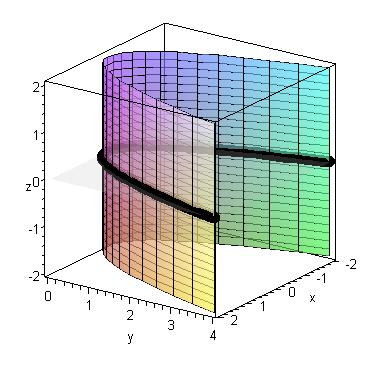
\includegraphics[width=\mywidth]{functions/cylinder-1}&
%%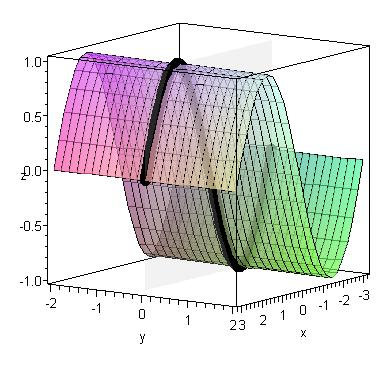
\includegraphics[width=\mywidth]{functions/cylinder-2}&
%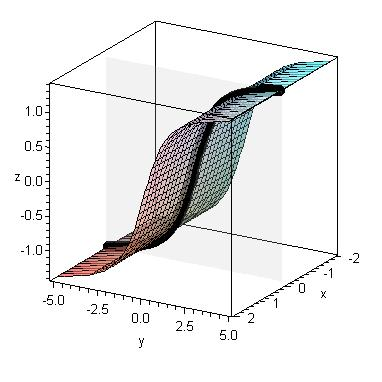
\includegraphics[width=\mywidth]{functions/cylinder-3}&
%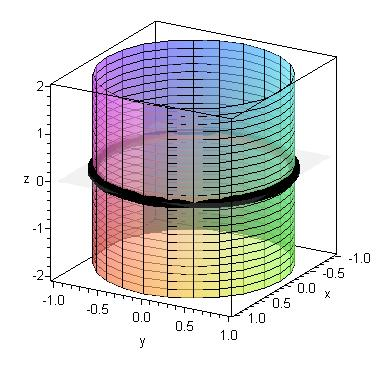
\includegraphics[width=\mywidth]{functions/cylinder-4}
\\
$y=\tan(z)$ &
$x^2+y^2=1$
\end{tabular}
\end{center}

\subsection{Quadric Surfaces}
A quadric surface is a generalization of a conic section to three
dimensions.  In general, it is the graph in 3D of any expression
involving at most second degree terms in $x$, $y$, and/or $z$. To
graph a quadric surface, hold one variable constant and then graph the
resulting conic section in the plane which represents the variable you
held constant. Repeat this for a few different variables and constants
until you can piece together the surface.  An example of this process
for $\frac{x^2}{4}+\frac{y^2}{9}-z^2 =1$ is illustrated below, as well
as some typical quadric surfaces.  \renewcommand{\mywidth}{.9in}
\begin{center}
\begin{tabular}{cccc}

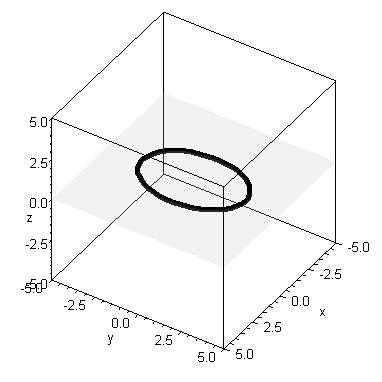
\includegraphics[width=\mywidth]{functions/quadric-1}&
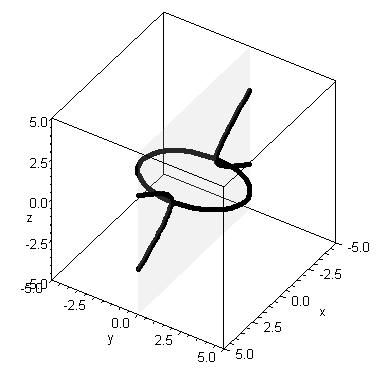
\includegraphics[width=\mywidth]{functions/quadric-2}&
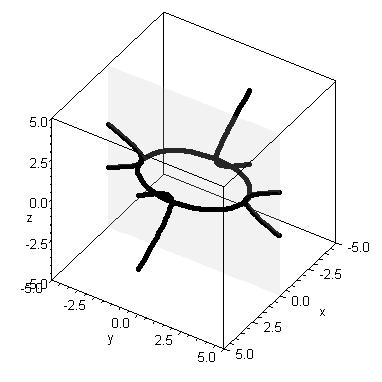
\includegraphics[width=\mywidth]{functions/quadric-3}&
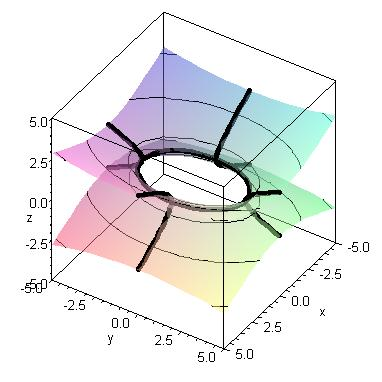
\includegraphics[width=\mywidth]{functions/quadric-4}
\\
Let $z=0$ &
Let $y=0$ &
Let $x=0$ &
$\frac{x^2}{4}+\frac{y^2}{9}-z^2 =1$\\
&&&Hyperboloid of one sheet
\\
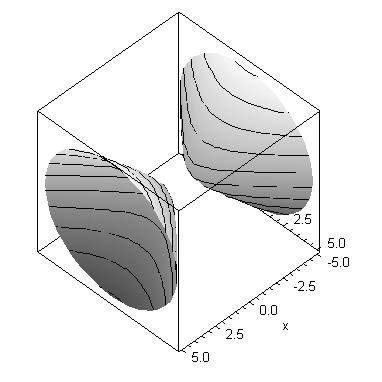
\includegraphics[width=\mywidth]{functions/quadric-5}&
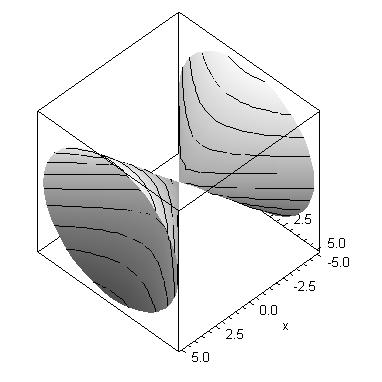
\includegraphics[width=\mywidth]{functions/quadric-6}&
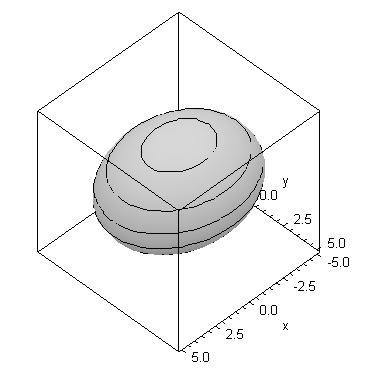
\includegraphics[width=\mywidth]{functions/quadric-7}&
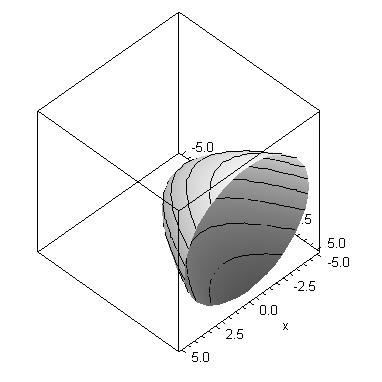
\includegraphics[width=\mywidth]{functions/quadric-8}
\\
$x^2-y^2-z^2=1$ &
$-x^2+y^2+z^2=0$ &
$\frac{x^2}{25}+\frac{y^2}{16}+\frac{z^2}{9}=1$ &
$x^2-4y+z^2=1$
\\
Hyperboloid of 2 sheets&
Cone &
Ellipsoid &
Paraboloid
\end{tabular}
\end{center}






\section{Function terminology}
A function is a set of instructions (a relation) involving two sets
(called the \emph{domain} and \emph{codomain}).  A function assigns to
each element of the domain $D$ at most one element in the codomain
$R$. It is customary to write {$f\colon D\to R$} when we want to
specify the domain and codomain.  Not all elements of $R$ may be
assigned; the set of elements in $R$ that are assigned is called the
\emph{range} or \emph{image} of the function.
\note{drawing of the domain, range, and codomain circles, with the function arrow going between}

\begin{example}
  If the function $f(x)=x^2$, then the domain and codomain are typically
  $\RR$ (i.e., $f\colon \RR \to \RR$), and the range is the set of nonnegative numbers.
\end{example}

In this class, we will study what happens when the domain and codomain
are subsets of {${\RR}^n$} ($\RR^n$ is the set of all $n$-dimensional
real points, and is often called ``Euclidean {$n$}-space''). In
particular we will study functions of the form $f\colon {\RR}^n\to
{\RR}^m$.

\section{Functions: $\RR^n\to \RR$}
\subsection{Functions of one variable: $f\colon \RR^1\to  \RR^1$}
In the first year of calculus, the domain and codomain are always
subsets of the real numbers {$\RR$}.  A typical example is $f(x)=x^2$.
Many ideas like derivatives, integrals, etc., from first semester
calculus generalize to all dimensions, but some do not.

\subsection{Functions of several variables: \\ $f\colon \RR^2\to \RR$, $f\colon \RR^3\to \RR$, $f\colon \RR^n\to \RR$} 

With functions of this type, the output dimension is always 1, while
the input dimension may be as large as needed. This type of function
is used to measure a quantity at each point in the plane ($f\colon {\RR}^2\to
{\RR}$), at each point in space ($f\colon {\RR}^3\to {\RR}$), or for every
combination of $n$ inputs ($f\colon {\RR}^n\to {\RR}$). The temperature at
each point in the plane would be modeled by such a function of the
form $T(x,y)$. The wind speed at each point in space could be modeled
by a function of the form $f(x,y,z)$.

To graph functions of the form {$f\colon {\RR}^2\to {\RR}$}, we typically
write $z=f(x,y)$ and then plot the function in $xyz$ coordinates.
Every pair $(x,y)$ corresponds to exactly one point $(x,y,f(x,y))$ in
space.  Functions of this form still pass the ``vertical line test''
(where ``vertical line'' means a line parallel to the $z$-axis).  We
get 2D traces (vertical cross sections) of the function by replacing
$x$ or $y$ with a constant and creating a 2D graph of the resulting
function.  A level curve is a graph in the plane of the equation
$c=f(x,y)$ for some constant $c$ (essentially a level curve is a
horizontal cross section drawn in the $xy$-plane). Plotting several
level curves creates a \emph{contour plot} of the function.  A few
graphs and corresponding contour plots follow.


\renewcommand{\mywidth}{1.1in}
\begin{center}
\begin{tabular}{ccccc}
\tikzsetfigurename{functions-}
\begin{tikzpicture} 
 \begin{axis}[footnotesize, view={60}{30}, colormap/blackwhite] 
   \addplot3[surf,domain=-3:3,y domain=-3:3] {9-x*x-y*y}; 
 \end{axis} 
 \end{tikzpicture}
&
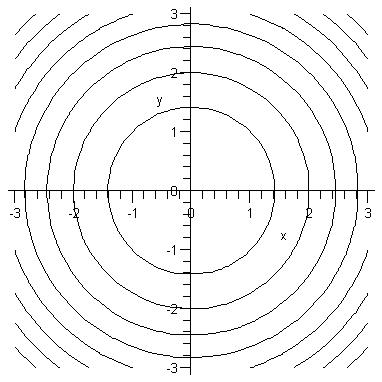
\includegraphics[width=\mywidth]{functions/functionseveral-2}&
\begin{tikzpicture} 
  \begin{axis}[footnotesize, view={60}{30}, colormap/blackwhite] 
    \addplot3[surf,domain=-2*pi:2*pi,y domain=-2*pi:2*pi] {sin(deg(x))*cos(deg(y))}; 
  \end{axis} 
\end{tikzpicture}&
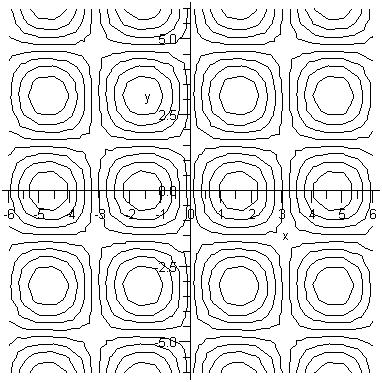
\includegraphics[width=\mywidth]{functions/functionseveral-4}
\\
$f(x,y)=9-x^2-y^2$&
level curves of $f$ &
$g(x,y) = \sin x \cos y$ &
level curves of $g$\end{tabular}
\end{center}

Functions with three inputs {$f\colon {\RR}^3\to {\RR}$} would require 4
dimensions to graph.  Rather than graph functions in 4D, we instead
look at level surfaces. For the function $w=f(x,y,z)$, we pick a
constant $w=c$ and graph the surface $c=f(x,y,z)$.  The level surface
$w=1$ for the function $f(x,y,z)=x^2+y^2+z^2$ is a sphere of radius 1
(given by graphing $x^2+y^2+z^2=1$).  Quadric surfaces will show up
often when you graph level surfaces of functions with three inputs.


\section{Parametric Functions}

\subsection{Parametric curves: {$\vec r\colon \RR\to \RR^2$}}
Parametric curves often represent motion in the plane.  We can write
these functions by giving the equations for each coordinate
separately, or we can write all of the equations as a vector, where
each coordinate of the vector is a function of one variable.  Because
the output of these functions is a vector, we call these functions
\emph{vector-valued functions}, and often emphasize this by writing
them with a vector symbol over the name.


\begin{example}
  The parametric curve $x=2\cos t$, $y=3\sin t$ traces out an ellipse.
  We can also write this in vector form as $\vec r(t) = \langle2\cos
  t, 3\sin t\rangle$.
\end{example}

\subsection{Spacecurves: {$\vec r\colon \RR\to \RR^3$}}
Space curves generalize parametric curves, but the outputs are
three-dimensional points, so these are curves in space.  The notation
{$\vec r\colon \RR \to \RR^3$} suggests that we are graphing a
one-dimensional object in three dimensions. The graph of a space curve
looks like a bent wire in space, or as a path of motion traced out in
space.  For each time $t$, the position vector $\vec r(t)$ gives the
position of a particle whose motion is described by the space curve.
Again, since the output is a vector, a space curve is a vector-valued
function.  Just like a 2D parametric plot, a space curve can graphed
by picking values for $t$ and plotting the corresponding points $\vec
r(t)$.

The derivative of a space curve is found by differentiating each
component of the space curve, which follows immediately by looking at
the limit $\ds\frac{d\vec r}{dt}=\lim_{h\to 0}\frac{\vec r(t+h)-\vec
  r(t)}{h}$. An equation of the tangent line to a space curve at $t=c$
has direction vector equal to $\dfrac{d\vec r}{dt}$ (evaluated at
$t=c$) and passes through the point $\vec r(c)$, and so has an equation of
$\vec l(u) = \vec r^\prime(c)u+\vec r(c)$. If a space curve is used to
describe motion, then velocity is $\vec v(t) = \dfrac{d\vec r}{dt}$,
speed is the magnitude of velocity $|\vec v|$, and acceleration is
$\vec a(t) = \dfrac{d\vec v}{dt}$, just as was taught in first-semester
calculus for single-variable functions.

\begin{example}
%\pgfplotsset{
%every axis style= {view/h=-45}}

\marginpartop{\begin{tikzpicture} 
    \begin{axis}[footnotesize, colormap/blackwhite, view/h=-40,
      xlabel=$x$, ylabel=$y$] 
      % tangent line
     \addplot3[mark=>] coordinates {(-0.0669872981077807, 1.11602540378444,
       1.59439510239320) (-0.933012701892219, 0.616025403784439,
       2.59439510239320)}; 
     % acceleration vector
     \addplot3[mark=>] coordinates {(-0.500000000000000, 0.866025403784439,
       2.09439510239320) (0.000000000000000, 0.000000000000000,
       2.09439510239320)};
     \addplot3[domain=0:4*pi, samples y=0, smooth] 
      ({cos(deg(x))}, {sin(deg(x))}, {x}); 
   \end{axis} 
  \end{tikzpicture}}%

% sage: r(t)=(cos(t), sin(t), t)
% sage: v=diff(r,t)(2*pi/3)
% sage: p=r(2*pi/3)
% sage: l=v*t+p
% sage: l(t=-0.5).n()
% (-0.0669872981077807, 1.11602540378444, 1.59439510239320)
% sage: l(t=0.5)
% (-0.250000000000000*sqrt(3) - 1/2, 1/2*sqrt(3) - 0.250000000000000, 2/3*pi + 0.500000000000000)
% sage: l(t=-0.5).n()
% (-0.0669872981077807, 1.11602540378444, 1.59439510239320)
% sage: a=diff(r,t,2)
% sage: print '%s %s'%(p.n(), (p+a(2*pi/3)).n())
% (-0.500000000000000, 0.866025403784439, 2.09439510239320) (0.000000000000000, 0.000000000000000, 2.09439510239320)


The space curve {$\vec r(t)=\langle\cos(t),\sin(t),t\rangle$} is a
helix which wraps around the $z$-axis.  Its graph is shown in the
margin, where $0\leq t\leq 4\pi$, as well as the tangent line and
acceleration vector. The velocity and acceleration at any time $t$ are
$\vec v(t) = \langle-\sin(t),\cos(t),1\rangle$ and $\vec a(t) =
\langle-\cos(t),-\sin(t),0\rangle$. When $t=2\pi/3$, we have $\vec
r(2\pi/3) = \langle1/2,\sqrt{3}/2,2\pi/3\rangle$, $\vec v(2\pi/3) =
\langle-\sqrt{3}/2,-1/2,1\rangle$, and $\vec a(2\pi/3) =
\langle1/2,-\sqrt{3}/2,0\rangle$. An equation of the tangent line is
$\vec l(t) = \vec v(2\pi/3)t+ \vec r(2\pi/3)=
\langle-\sqrt{3}/2,-1/2,1\rangle
t+\langle1/2,\sqrt{3}/2,2\pi/3\rangle$.
\end{example}


\subsection{Parametric Surfaces: {$\vec f\colon {\RR}^2\to {\RR}^3$} }

Just as parametric and space curves describe one-dimensional objects, we use parametric surfaces to describe two-dimensional objects in 3D.  Notice that we are mapping two dimensions into three, so think of a parametric surface as a set of instructions of how to place the 2D plane in space (where you can twist the plane and stretch it based on the set of instructions).  If you hold one variable constant, then the graph of the resulting function is a space curve. To graph a parametric surface, hold one variable constant and draw the resulting space curve.  Do this for a few values of each variable, and you will have created a net of overlapping space curves from which you can piece together the surface.  

Any surface of the form $z=f(x,y)$ can be made a parametric surface by
writing $\vec r(x,y)=\langle x,y,f(x,y)\rangle$, which just says for
each $(x,y)$ to plot the point $(x,y,f(x,y))$. We often use $u$ and
$v$ as variables for a parametric surface if those variables do not
represent some other standard quantity.

{
\tikzsetfigurename{parametricsurface-}
\begin{center}
\begin{tabular}{cccc}
\begin{tikzpicture} 
  \begin{axis}[footnotesize, view/h=-40,colormap/blackwhite] 
    \addplot3[surf,domain=-4:4,y domain=-4:4] 
    (x,y,{9-x^2-y^2}); 
  \end{axis} 
\end{tikzpicture}&

\begin{tikzpicture} 
  \begin{axis}[footnotesize, view/h=-40, colormap/blackwhite, z buffer=sort] 
    \addplot3[surf,domain=0:3,y domain=0:2*pi] 
    ({x*cos(deg(y))},{x*sin(deg(y))}, {9-x^2}); 
  \end{axis} 
\end{tikzpicture}\\
\parbox{0.5\textwidth}{\centering $\vec r(x,y) = \langle
  x,y,9-x^2-y^2\rangle$\\$-4\leq x\leq 4$, $-4\leq y\leq 4$}
&
\parbox{0.5\textwidth}{\centering $\vec r(u,v)=\langle u\cos v,u\sin v
  ,9-u^2\rangle$\\
  $0\leq u\leq 3$, $0\leq v\leq 2\pi$\\ 
  (cylindrical coordinates)}
\\[12pt]


\begin{tikzpicture} 
  \begin{axis}[footnotesize, view/h=-40, colormap/blackwhite, 
    z buffer=sort, variable=θ, variable y=φ] 
    \addplot3[surf,domain=0:2*pi,y domain=pi/4:3*pi/4] 
    ({3*cos(deg(θ))*sin(deg(φ))},{3*sin(deg(θ))*sin(deg(φ))},{3*cos(deg(φ))});
 \end{axis} 
\end{tikzpicture}&

\begin{tikzpicture} 
  \begin{axis}[footnotesize, view/h=-40, z buffer=sort, colormap/blackwhite] 
    \addplot3[surf,domain=0:2*pi,y domain=0:pi] 
    ({x*sin(deg(x))*cos(deg(y))},{x*cos(deg(x))*cos(deg(y))}, {x*sin(deg(y))}); 
  \end{axis} 
\end{tikzpicture}\\

\parbox{0.5\textwidth}{\centering $\vec
  r(\theta,\phi)=\langle3\cos\theta\sin\phi,3\sin\theta\sin\phi,3\cos\phi\rangle$\\
  $0\leq \theta\leq 2\pi$, $\frac{\pi}{4}\leq \phi\leq \frac{3\pi}{4}$
  \\
  (spherical coordinates) } 
&

\parbox{0.5\textwidth}{\centering $\vec r(u,v)=\langle u\sin u \cos v
  , u\cos u \cos v , u\sin v \rangle$\\
 $0\leq u\leq 2 \pi$, $0\leq v\leq \pi$}



\end{tabular}
\end{center}
}

\section{Functions: $\RR^n\to \RR^n$}

\subsection{Transformations (changing coordinates)\\ {$\vec f\colon \RR^2\to \RR^2$}, {$\vec f\colon \RR^3\to \RR^3$}}

The polar coordinate equations $x=r\cos\theta$, $y=r\sin\theta$
require two inputs $(r,\theta)$ and give two outputs $(x,y)$.  This can
be thought of as a function $T(r,\theta)=\langle
r\cos\theta,r\sin\theta\rangle$. Every time we change coordinate
systems, it will be valuable to give that tranformation a name and
recognize that it is really a function.

\note{drawing showing a transformation of the $r,\theta$ plane to the $x,y$ plane}

\subsubsection{Cylindrical Coordinates}
Cylindrical coordinates is an extension of polar coordinates to three
dimensions.  The transformation $T(r,\theta,z) = \langle
r\cos\theta,r\sin\theta,z\rangle$ gives us a new way of viewing points
in 3D.  Using the triangle $x,y,r$, we can figure out the following
relationships.
\begin{align*}
  x&=r \cos \theta & 
  y&=r \sin \theta & 
  \tan\theta&=y/x & 
  r^2&=x^2+y^2     
\end{align*}

\begin{example}
The cylindrical point {$(r, \theta, z)=(3,\pi/2,4)$} in
cylindrical coordinates is the same as the rectangular point $(x,y,z)
= (0,3,4)$.
\end{example}

\subsubsection{Spherical Coordinates}
Spherical coordinates $(\rho,\theta,\phi)$ are defined as follows.
The distance (\emph{radius}) from the origin to the point $(x,y,z)$ is
called $\rho$. The angle $\theta$ (the \emph{azimuth}) is the same as
in polar or cylindrical coordinates. The angle $\phi$ (the
\emph{inclination}) is the angle between the positive $z$-axis and a
ray from the origin to $(x,y,z)$. Using these definitions, we obtain
the following equations by considering the two right triangles with
edges $x,y,r$ and $r,z,\rho$:\note{draw nice pictures of the variables for cylindrical and spherical coordinates}
\begin{align*}
  x&=\rho\sin\phi\cos\theta  &
  y&=\rho\sin\phi\sin\theta & 
  z&=\rho\cos\phi\\
  \tan\theta&=y/x &
  r&=\rho\sin\phi & 
  \rho^2&=x^2+y^2+z^2 &
\end{align*}
We can describe the spherical coordinate transformation as a
function 
$$T(\rho,\theta,\phi) = \langle\rho\sin\phi\cos\theta,\rho\sin\phi\sin\theta,\rho\cos\phi\rangle.$$ 

\begin{example} 
The spherical point {$(\rho, \theta, \phi)=(4,\pi,\pi/4)$} is the same
as the rectangular point $(x,y,z) = (4/\sqrt{2},0,4/\sqrt{2})$.
\end{example}

There is some disagreement in different fields about the notation for
spherical coordinates.  In some fields, $\phi$ represents the azimuth
angle and $\theta$ represents the inclination angle (or the
\emph{elevation} angle---the angle from the $xy$-plane).
Additionally, sometimes the coordinates are written in a different
order.  You should always check the notation for spherical coordinates
before communicating using them.
\note{draw some nice plots illustrating the transformation in 3d}

\subsubsection{Graphing in other coordinate systems}
To graph an equation in a different coordinate system, simply substitute the equation into the transformation and graph the result as a parametric surface.  

\begin{example}
Suppose we have the spherical coordinate equation $\rho(\theta,\phi)=3\phi^2\cos\theta$.  Subsituting this in for $\rho$ in the transformation function gives 
\begin{align*}
T(\theta,\phi) &= \langle\rho(\theta,\phi)\sin\phi\cos\theta, \rho(\theta,\phi)\sin\phi\sin\theta, \rho(\theta,\phi)\cos\phi\rangle\\
&=\langle3\phi^2\cos\theta\sin\phi\cos\theta, 3\phi^2\cos\theta\sin\phi\sin\theta, 3\phi^2\cos\theta\cos\phi\rangle\\
\end{align*}
\end{example}
 
You can see two examples of graphing $z=9-r^2$ (cylindrical
coordinates, where $u=r$ and $v=\theta$) and $\rho=3$ (spherical
coordinates) in the parametric surfaces section.

\subsection{Vector Fields: {$\vec f\colon \RR^2\to \RR^2$}, {$\vec f\colon \RR^3\to \RR^3$}}
Another way to represent a function mapping $\RR^n\to\RR^n$ is as a
vector field.  A vector field $\vec F(x,y) = \langle
M(x,y),N(x,y)\rangle$ or $\vec F(x,y,z) = \langle
M(x,y,z),N(x,y,z),P(x,y,z) \rangle$ is a function which assigns to
each point in the plane (or space) a vector.  Vector fields are used
to model gravity, forces, velocity, wind, acceleration, electric
fields, and many other things in nature. For example, the speed and
direction of wind depends on location, so the velocity of wind can be
represented by drawing a bunch of vectors at different points on a
map.  Vector fields may be one of the most useful tools we have.  You
should practice creating vectors given a description. 

\begin{example} 
A vector field in the plane in which the vector at any
point is directed towards the origin and has magnitude equal to the
square of the distance to the origin is
$$\vec F(x,y) =
(x^2+y^2)\frac{\langle-x,-y\rangle}{\sqrt{x^2+y^2}}.$$ We constructed
the equation for the vector field by expressing the vector at the
point $(x,y)$ as a magnitude times a unit direction vector.  
\end{example}

To graph a vector field $\vec F(x,y) = \langle M,N\rangle$ in the
plane, at each point $(x,y)$, we draw the vector $\vec F(x,y)$ at the
point $(x,y)$. Since the vectors may be rather long, computers will
proportionally rescale all vectors so that the vectors fit in the
graph.

% \begin{sagesilent}
%   mathematica('myplot = VectorPlot[{y, -x}, {x, -3, 3}, {y, -3, 3}]')
%   mathematica('Export["%s/functions-mma/field-circle.pdf", myplot]' % os.getcwd())
% \end{sagesilent}
%\includegraphics[width=\mywidth]{functions-mma/field-circle}
\begin{sagesilent}
var('x,y,z')
r=sqrt(x^2+y^2+z^2)
\end{sagesilent}
\renewcommand{\mywidth}{1.4in}
\begin{center}
\begin{tabular}{cccc}
\sageplot[width=\mywidth]{plot_vector_field((-y,x), (x,-5,5),(y,-5,5),pivot='middle'),aspect_ratio=1,figsize=2} &
\sageplot[width=\mywidth]{plot_vector_field((2*x+y,x-y), (x,-5,5),(y,-5,5),pivot='middle'),aspect_ratio=1,figsize=2} &
\sageplot[width=\mywidth][png]{plot_vector_field3d((-x/r,-y/r,-z/r), (x,-5,5),(y,-5,5),(z,-5,5),colors='black')}&
\sageplot[width=\mywidth][png]{plot_vector_field3d((y,z,x), (x,-5,5),(y,-5,5),(z,-5,5),center_arrows=True,colors='black')}
\\
$\vec F(x,y)=\langle-y,x\rangle$&
$\vec F(x,y)=\langle2x+y,x-y\rangle$&
$\vec F(x,y,z)=\frac{\langle-x,-y,-z\rangle}{\sqrt{x^2+y^2+z^2}}$&
$\vec F=\langle y,z,x \rangle$
%$F=\langle-x+y,-yz+1,z\rangle$
\end{tabular}
\end{center}
\note{use the subfigure environment}








%%% Local Variables: 
%%% mode: latex
%%% TeX-master: "../multivariable-calculus"
%%% End: 






\newgeometry{left=1in,right=1in,top=1in,bottom=1in}
\newpage

\section{Preparation}

\subsection{Lesson Plans}

This chapter covers the following ideas. When you create your lesson plan, it should contain examples which illustrate these key ideas. Before you take the quiz on this unit, meet with another student out of class and teach each other from the examples on your lesson plan. 

% A list of objectives for the chapter
%\begin{enumerate}
%\item ...
%\end{enumerate}


\begin{enumerate}
\item Be able to describe cylinders and quadric surfaces in space.
\item Describe uses for function with varying input and output
  dimensions.  Be able to draw appropriate representations when the
  input and output dimensions are 3 or less. Recognize by name and
  graph the different types of functions, in particular parametric
  equations, space curves, functions of several variables, vector
  fields, transformations, and parametric surfaces.
\item Find derivatives of space curves, and use the derivative to find
  tangent lines to space curves.
\end{enumerate}


%%% Local Variables: 
%%% mode: latex
%%% TeX-master: "../multivariable-calculus"
%%% End: 
%$


%\subsection{Preparation Problems}

%Here are the preparation problems for this unit.

\subsection{Homework}

In the following list, the ``basic practice'' problems should be quick
problems to help you master the ideas.  The ``good problems'' will
require a little more work.  The theory and application problems are
ones that will challenge you more; make sure you do the problems from
this area to fully master the material.  

{\noindent \footnotesize \begin{tabular}{|p{1.35in}|c|p{1.2in}|p{1.2in}|p{1.5in}|l|}\hline
Topic &Sec &Basic Practice &Good Problems &Thy/App \\\hline
Surfaces & 11.6 & 1--16, 31--40 & 19--30, 41--44 & 53--54, 56, 63--66\\\hline
Vector-valued functions & 12.1 & 1--42 & 43--68 & 81--83, 89--92\\\hline
& 12.2 & 1--26 & &\\\hline
& 12.3 & 1--16 & & \\\hline
& 12.4 & 19--20 & & \\\hline
Several variables& 13.1 & 1--28, 31--42, 45--48, 57--60 & 29--30, 43--44, 49--56, 65--66, 69--74 & 61--64, 67--68, 75--92\\\hline
Transformations & 11.7 & 1--12, 29--40, 57--72 & 73--86 & 121--122, Derive equations for cylindrical and spherical coordinates\\\hline
Vector Fields & 15.1 & 1--20 & & \\\hline
Parametric surfaces & 15.5 & 1--4, 9--18 & & 46--48, 53--54\\\hline
\end{tabular}
}




%%% Local Variables: 
%%% mode: latex
%%% TeX-master: "../multivariable-calculus"
%%% End: 


%%% Local Variables: 
%%% mode: latex
%%% TeX-master: "../multivariable-calculus"
%%% End: 

\restoregeometry


\chapter{Derivatives}

This chapter covers the following ideas.  When you make your lesson
plan, it should cover all of these objectives.

% A list of objectives for the chapter
%\begin{enumerate}
%\item ...
%\end{enumerate}

\begin{enumerate}
\item Find limits and determine where functions of several variables
  are continuous.
\item Compute partial derivatives.  Use them to find tangent lines and
  tangent planes.
\item Be able to find the derivative of a function (as a matrix) and
  use it to find tangent planes.
\item Find derivatives of composite functions using the chain rule
  (matrix multiplication).
\item Find derivatives when constraints are in a problem.
\end{enumerate}

%%% Local Variables: 
%%% mode: latex
%%% TeX-master: "../multivariable-calculus"
%%% End: 
%$




\section{Limits and Continuity}
We start with some notation.  We will denote functions using $\vec f\colon
\mathbb{R}^n\to\mathbb{R}^m$ where $n$ is the number of inputs, and $m$
is the number of outputs.  We will use $\vec x$ to represent an input,
and $\vec y$ to represent an output.  For example, if $z=f(x,y)$, then
in vector notation we would write $\vec y=\vec f(\vec x)$, where $\vec
y=\langle z\rangle$ and $\vec x = \langle x,y\rangle$.  The parametric
surface $\vec r(u,v)=\langle x,y,z\rangle$ would be written as $\vec
f(\vec x)=\vec y$ where $\vec x = \langle u,v\rangle$ and $\vec
y=\langle x,y,z\rangle$.  Using this notation allows us to restate most
of the theorems of multivariable calculus using the exact same
notation as was learned in single variable calculus.

Recall that in first semester calculus, we defined the limit of a
function by saying that a function $y=f(x)$ has limit $L$ at $x=c$ if
for every $\epsilon>0$, there exists a $\delta>0$ such that if $0<|x-c|<\delta$, then
$|f(x)-L|<\epsilon$. The idea is that you can make the output value $y$ as
close to $L$ as you want (i.e., within $\epsilon$ of $L$) by requiring the
input values $x$ to be very close to $c$ (i.e., within $\delta$ of $c$).
This definition generalizes to all dimensions by placing vector
symbols above everything.  We say that a function $\vec y=\vec f(\vec
x)$ has limit $\vec L$ at $\vec x=\vec c$ if for every $\epsilon>0$, there
exists a $\delta>0$ such that if $0<|\vec x-\vec c|<\delta$, then $|\vec f(\vec
x)-\vec L|<\epsilon$. We interpret absolute values as distance (the square
root of the dot product). Learning to use the formal limit definition
to prove theorems about limits and derivatives will be deferred to a
course in real analysis, where an appropriate amount of time can be
spent on the topic. For now, the main idea is that a function has a
limit of $\vec L$ at $\vec c$ if the $\vec y$ values are close to
$\vec L$ for all $\vec x$ values close enough to $\vec c$.  We say
that a function is continuous at $\vec x=\vec c$ if the limit of the
function $\vec L$ equals $\vec f(\vec c)$ (i.e., $\lim_{\vec x \to \vec
  c}\vec f(\vec x)=\vec f(\vec c)$; we could just calculate the limit
by plugging in $\vec x=\vec c$).

The main difference between single-variable limits and multivariable
limits is that when there is only one input variable, you can study
limits from the left and limits from the right---those are the only
ways $x$ can move closer to $c$.  However, if there are more input
variables, then there are infinitely many ways to approach $\vec c$. A
limit exists at $\vec c$ if and only if the limit exists along
\emph{every} approach to $\vec c$.  For example, the function $f(x,y)
= \frac{x^2-y^2}{x^2+y^2}$ has a limit at every point in the plane
except at the origin because rational functions are continuous as long
as the denominator is nonzero.  We write $\ds
\lim_{(x,y)\to(a,b)}\frac{x^2-y^2}{x^2+y^2}=\frac{a^2-b^2}{a^2+b^2}$ as
long as $(a,b)\neq(0,0)$.  If $(a,b)=(0,0)$, then we will consider two
different ways of approaching the origin.  If we look at $(x,y)$
values on the $x$-axis, then we write $\ds
\lim_{\text{\tiny$\begin{array}{c} (x,y)\to(a,b)\\y=0
\end{array}$}} 
\frac{x^2-y^2}{x^2+y^2} = \lim_{x\to 0} \frac{x^2}{x^2}=1$.
Alternatively, if we look at $(x,y)$ values on the $y$-axis, then we
write 
$\ds \lim_{\text{\tiny$\begin{array}{c}
 (x,y)\to(a,b)\\x=0
\end{array}$}} \frac{x^2-y^2}{x^2+y^2} = \lim_{y\to 0}
\frac{-y^2}{y^2}=-1$. Hence we see that the limit is not the
same for different approaches.  In fact, if we only consider $(x,y)$
values on the line $y=mx$ for any $m$, then we write 
$\ds \lim_{\text{\tiny$\begin{array}{c}
 (x,y)\to(a,b)\\y=mx
\end{array}$}} \frac{x^2-y^2}{x^2+y^2} = \lim_{x\to 0}
\frac{x^2-(mx)^2}{x^2+(mx)^2}=\frac{1-m^2}{1+m^2}$, which is different
for each $m$. We say that the function $f$ has no limit (or the limit is undefined) at the
origin because the limit is not the same along different approaches. 

If a function has a limit, then the limit will be the same regardless
of the approach. In the functions below, the first does not have a
limit at the origin, the second does, and the third is discontinuous
along an entire curve $y=x^2$.

\begin{center}
\begin{tabular}{ccc}
\tikzsetfigurename{limits-}
\remake
\begin{tikzpicture} 
  \begin{axis}[footnotesize, view/h=-20,xlabel=$x$,ylabel=$y$] 
   \addplot3[surf,domain=-1:1,y domain=-1:1] (x,y,{(x^2-y^2)/(x^2+y^2)}); 
\end{axis} 
\end{tikzpicture}&
\remake

\begin{tikzpicture} 
  \begin{axis}[footnotesize, view/h=-40, xlabel=$x$,ylabel=$y$] 
    \addplot3[surf,domain=-1:1,y domain=-1:1] (x,y,{(x^2*y)/(x^2+y^2)}); 
 \end{axis} 
 \end{tikzpicture}&
 \remake
\begin{tikzpicture} 
  \begin{axis}[footnotesize, view/h=-40,
    xlabel=$x$,ylabel=$y$,restrict z to domain*=-5:5,samples=50] 
    \addplot3[surf,domain=-1:1,y domain=-1:1] (x,y,{(x)/(y+x^2)}); 
 \end{axis} 
 \end{tikzpicture}\\

$f(x,y)=\frac{x^2-y^2}{x^2+y^2}$ &
 $f(x,y)=\frac{x^2y}{x^2+y^2}$ &
 $f(x,y)=\frac{x}{x^2-y}$\\
\end{tabular}
\end{center}


\section{Partial Derivatives} 
If a function $f$ has only one input $x$, then the derivative is
defined to be $\ds \frac{d f}{dx} = \lim_{h\to 0}\frac{f(x+h)-f(x)}{h}$.
The derivative gives the best possible linear approximation to changes
in a function. This idea is represented by the equation $\Delta  y \approx
f^\prime(x)\Delta x$, or in differential form, we write $d y=f^\prime(x) dx$.  An
equation of a tangent line is found by noticing that a change in $y$
is approximately $y-f(c)$ when the change in $x$ is $x-c$, so the
differential form $dy=f^\prime dx$ becomes $(y-f(c))=f^\prime(c)(x-c)$.  I
repeat, the derivative gives the best possible linear approximation to
changes in a function.

If a function has more than one input variable, then division by the
vector $\vec h$ is not well-defined, so we run into a problem with
generalizing derivatives.  Instead, we start with partial derivatives,
which approximate change in the function if we hold all other
variables constant and just differentiate with respect to one
variable.  For the function $f(x,y)$, we define the partial derivative
of $f$ with respect to $x$ as $\ds f_x(x,y)=f_x = \frac{\partial f}{\partial x}=
\lim_{h\to 0}\frac{f(x+h,y)-f(x,y)}{h}$, and the partial derivative of
$f$ with respect to $y$ as $\ds f_y(x,y)=f_y =\frac{\partial f}{\partial y}=
\lim_{k\to 0}\frac{f(x,y+k)-f(x,y)}{k}$. Notice that $f_x$ computes a
limit as $y$ is held constant and we vary $x$. For
$f(x,y)=3x^2+4xy+\cos(xy)+y^3$, we obtain $f_x=6x+4y-y\sin(xy)+0$ and
$f_y=0+4x-x\sin(xy)+3y^2$. Partial derivatives are found by holding
all other variables constant, and then differentiating with respect to
the variable in question. Practice computing partial derivatives with
lots of functions. The homework should go very quickly, but this skill
needs plenty of practice so that partial differentiation is done
immediately.

Partial derivatives approximate change in a function as you vary only
one variable, hence a partial derivative gives slope in the direction
which is varied. For the function $z=f(x,y)$, $f_x$ is the slope of a
line tangent to the surface $z=f(x,y)$, where the tangent line is
parallel to the $xz$-plane. A direction vector for this line is
$\langle1,0,f_x\rangle$ (every increase in $x$ of 1 unit yields an
increase in the output $z$ of $f_x$ units, and $y$ does not change). 
Similarly $\langle0,1,f_y\rangle$ is a direction vector of a line
tangent to the surface, where the line is parallel to the $yz$-plane.
The cross product of these two vectors is $\vec n =
\langle-f_x,-f_y,1\rangle$, which is a normal vector for the tangent
plane to the surface. For the function $f(x,y)=9+x-y^2$ at
$(x,y)=(1,2)$, we have $f(x,y)=6$, $f_x(x,y) =1$, $f_y(x,y)=-2y$,
$f_x(1,2)=1$, and $f_y(1,2)=-4$. So a tangent line to the surface at
$(1,2,6)$ in the $x$ direction is $\vec r(t) = \langle1,0,1\rangle t+ 
\langle1,2,6\rangle$, in the $y$ direction is $\vec r(t) =
\langle0,1,-4\rangle t+  \langle1,2,6\rangle$, and an equation of the
tangent plane is $-1(x-1)+4(y-2)+1(z-6)=0$. The pictures below
illustrate these lines and planes 

\renewcommand{\mywidth}{1.3in}
\begin{center}
\begin{tabular}{ccc}
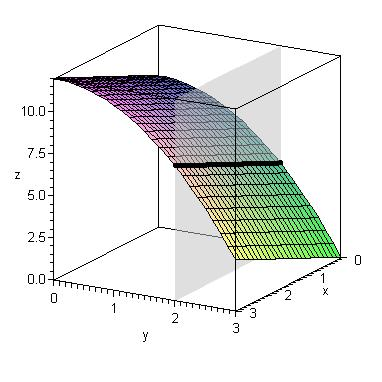
\includegraphics[width=\mywidth]{04-Derivatives/support/tan-1}&
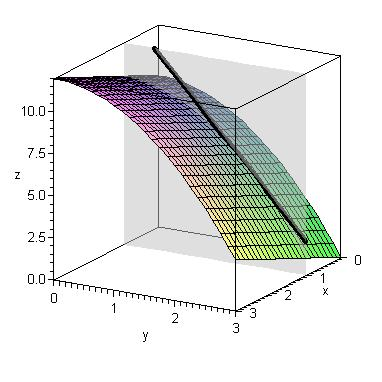
\includegraphics[width=\mywidth]{04-Derivatives/support/tan-2}&
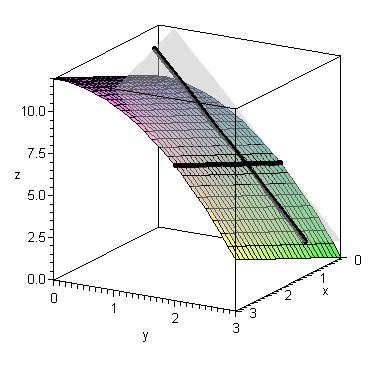
\includegraphics[width=\mywidth]{04-Derivatives/support/tan-3}
\\
$y$ is constant, $\vec v = \langle1,0,f_x\rangle$ &
$x$ is constant, $\vec v = \langle0,1,f_y\rangle$ &
Tangent plane $n=\langle-f_x,-f_y,1\rangle$
\end{tabular}
\end{center}



For the parametric surface $\vec r(u,v)=\langle u,v,9+u-v^2\rangle$, we
compute $\vec r_u = \langle1,0,1\rangle$ and $\vec r_v =
\langle0,1,-2v\rangle$, which are direction vectors for tangent lines
to the surface (notice they are the same vectors as in the previous
example).  At the point $(u,v)=(1,2)$, the tangent lines and tangent
plane are exactly the same as those for the function
$z=f(x,y)=9+x-y^2$. 

Since a partial derivative is a function itself, you can take
derivatives of a partial derivative as well, giving what is called
higher order partials.  For the function $f(x,y,z)=x^2+4xy^2-yz^3$, we
have $f_x=2x+4y^2, f_y=8xy-z^3, f_z=-3yz^2$, and so we obtain the
following second order partial derivatives $
\frac{\partial}{\partial x}f_x = f_{xx} = 2,
\frac{\partial}{\partial y}f_x = f_{xy} = 8y,
\frac{\partial}{\partial z}f_x = f_{xz} = 0,
\frac{\partial}{\partial x}f_y = f_{yx} = 8y,
\frac{\partial}{\partial y}f_y = f_{yy} = 8x,
\frac{\partial}{\partial z}f_y = f_{yz} = -3z^2, 
\frac{\partial}{\partial x}f_z = f_{zx} = 0, 
\frac{\partial}{\partial y}f_z = f_{zy} = -3z^2, 
\frac{\partial}{\partial z}f_z = f_{zz} = -6z.$
Notice that $f_{xy}=f_{yx}, f_{xz}=f_{zx}$, and $f_{zy}=f_{yz}$. As
long as a function is two times continuously differentiable, then
second order partial derivatives using the same variables but in a
different order will always be the same. This fact will get used
periodically throughout the class.

\section{The Derivative} 
The derivative of a function $\vec f:\mathbb{R}^n\to\mathbb{R}^m$ is an
$m\times n$ matrix, notated as $D\vec f(\vec x)$, where the columns of the
matrix are the partial derivatives of the function with respect to
each input variable (the first column is the partial derivative with
respect to the first variable, and so on). Some people call this
derivative the ``total'' derivative instead of the derivative, to
emphasize that the ``total'' derivative combines the ``partial''
derivatives into a matrix. This matrix is also called the Jacobian
matrix (or sometimes simply the Jacobian) of the function.  This
definition of the derivative gives the best possible linear
approximation to changes in a function. A full course in linear
algebra is needed to fully understand the significance of this
statement, however we can use the derivative as a matrix to simplify a
lot of our work in multivariable calculus.

Some examples of functions and their derivatives are in Table~\ref{tab:derivatives}. When the
output dimension of a function is one, then the matrix has only one
row. In this case, we often consider it as a row vector and the
derivative is called the gradient of $f$ and written $\nabla f$.  

\begin{table}[h]
  \centering
    \begin{tabular}{ll}\toprule
Function&Derivative\\ \midrule
{$f(x)=x^2$}& {$Df(x) = \begin{bmatrix}2x\end{bmatrix} $}\\ 
{$\vec r(t) = \langle3\cos(t),2\sin(t)\rangle$}&  {$D\vec r(t) =
\begin{bmatrix}-3\sin t\\ 2\cos t\end{bmatrix} $}\\ 
{$\vec r(t) = \langle\cos(t),\sin(t),t\rangle$}&  {$D\vec r(t) =
\begin{bmatrix}-\sin t \\ \cos t \\ 1\end{bmatrix} $}\\ 
{$f(x,y)=9-x^2-y^2$}&  {$Df(x,y) =\nabla f(x,y) = \begin{bmatrix}-2x &
-2y\end{bmatrix} $}\\ 
{$f(x,y,z)=x^2+y+xz^2$}&  {$Df(x,y,z) = \nabla f(x,y,z) =
\begin{bmatrix}2x+z^2 & 1 &2xz\end{bmatrix} $}\\ 
{$\vec F(x,y)=\langle-y,x\rangle$}&  {$D\vec F(x,y) =
\begin{bmatrix}0&-1\\ 1&0\end{bmatrix} $}\\ 
{$\vec F(r,\theta,z)=\langle r\cos\theta,r\sin\theta,z\rangle$}&  {$D\vec F(r,\theta,z) = 
\begin{bmatrix}
\cos \theta &-r\sin\theta&0\\ 
\sin\theta&r\cos\theta&0\\ 
0&0&1
\end{bmatrix} $}\\ 
{$\vec r (u,v)=\langle u,v,9-u^2-v^2\rangle$}&  {$D\vec r(u,v) =
\begin{bmatrix}1&0\\ 0&1\\ -2u&-2v\end{bmatrix} $}\\ 
      \\\bottomrule
    \end{tabular}

  \caption{Example derivatives}
  \label{tab:derivatives}
\end{table}

To emphasize that the derivative is the best possible linear
approximation to changes in a function, replace $f^\prime$ in the single
variable equation $dy=f^\prime dx$ with the derivative $D\vec f(\vec x)$ to
obtain $d\vec y =D\vec f(\vec x)d\vec x$ ($d[\text{outputs}]=Df
d[\text{inputs}]$).  For a function $z=f(x,y)$ we obtain
$dz=Df(x,y)\begin{bmatrix}dx\\dy\end{bmatrix} =
\begin{bmatrix}f_x&f_y\end{bmatrix}\begin{bmatrix}dx\\dy\end{bmatrix}
= f_xdx+f_ydy$ using matrix multiplication. To get an equation of a
tangent plane to a surface at $(a,b,f(a,b))$, we let $dz=z-f(a,b),
dx=x-a,dy=y-b$, and then obtain $z-f(a,b) =
\begin{bmatrix}f_x&f_y\end{bmatrix}\begin{bmatrix}x-a\\y-b\end{bmatrix}=f_x(a,b)
(x-a)+f_y(a,b)(y-b)$. This is equivalent to  $-f_x(a,b)
(x-a)-f_y(a,b)(y-b)+z-f(a,b)=0$, which is the equation of a plane with
normal vector $\vec n=\langle-f_x,-f_y,1\rangle$, which we already
obtained in the partial derivatives section. For the function
$f(x,y)=9+x-y^2$ at $(x,y)=(1,2)$, an equation of the tangent plane is
simply  $z-6 =
\begin{bmatrix}1&-4\end{bmatrix}\begin{bmatrix}x-1\\y-2\end{bmatrix}$. 
This version of finding tangent planes generalizes to all dimensions
and gives the ``tangent space.''

This optional paragraph explains why the definition of the derivative
above makes sense. Since division by $\vec h$ is not defined if $\vec
h$ is a vector and not a number, we modify the definition of the
derivative to define the derivative of a function in general. The
definition of the derivative when written using the formal definition
of a limit requires that we examine the inequality
$|\frac{f(x+h)-f(x)}{h} - f^\prime(x)|<\epsilon$.  Multiply both sides by $|h|$
and obtain $|f(x+h)-f(x) - f^\prime(x)h|<\epsilon|h|$. The derivative of a
function $\vec f:\mathbb{R}^n\to\mathbb{R}^m$ gives the best possible
linear approximation to changes in the function. A course in linear
algebra will show you that this means the derivative can be
represented by a matrix, and then the equation $|\vec f(\vec x+\vec
h)-\vec f(\vec x) - D\vec f(\vec x)\vec h|<\epsilon|\vec h|$ shows that
$D\vec f(\vec x)$ must be able to multiply on the right by vectors of
size $n$ (hence it has $n$ columns), and the product $D\vec f(\vec
x)\vec h$ must give a vector with $m$ components (hence the matrix has
$m$ rows). By considering the vector $\vec h =
\langle h_1,0,\ldots,0\rangle$, it can be shown that the first column of
$D\vec f(\vec x)$ equals the partial derivative of $\vec f$ with
respect to the first variable. 
 
\section{The Chain Rule}
For multivariable functions, we can form the composition $\vec f\circ \vec
g$ of two functions $\vec f:\mathbb{R}^n\to \mathbb{R}^m$ and $\vec
g:\mathbb{R}^p\to \mathbb{R}^n$ provided that output dimension of $\vec
g$ is the same as the input dimension of $\vec f$.  The composition
$\vec f(\vec g(\vec x))$ essentially asks us to put into the function
$\vec g$ a vector $\vec x$ of size $p$, which will give us a vector
$\vec g(\vec x)$ of size $n$.  Since this is the dimension of the
domain of $\vec f$, then we can put $\vec g(\vec x)$ into the function
$\vec f$, and we get a vector $\vec f(\vec g(\vec x))$ of size $m$.
For example, if $f(x,y)=x^2-y$ and $\vec
g(r,s,t)=\langle3r+4s,t^2-r\rangle$, then $f(\vec g(r,s,t)) =
f(3r+4s,t^2-r) = (3r+4s)^2-(t^2-r)$.

Recall from first semester calculus the chain rule: {$(f\circ g)^\prime(x) =
  f^\prime(g(x))g^\prime(x)$} (the derivative of the outside function multiplied
by the derivative of the inside function). The high-dimensional
version of the chain rule is exactly the same, namely {$D(\vec f\circ \vec
  g)(\vec x) = D\vec f(\vec g(\vec x))D\vec g(\vec x)$}, and a proof
is essentially the same (but we will leave this to another course).
The product is matrix multiplication. Most textbooks explain a rule
for remembering the multiplications involved in the chain rule, but
these are just ways of organizing matrix multiplication without
referring to a matrix.

We now look at a few examples. Suppose the temperature at each point
in the plane is given by {$f(x,y) = 9-x^2-y^2$}.  A particle moving
through the plane along the curve $x=t+1, y=t^2$ will have a
temperature given by $f(r(t)) = f(t+1,t^2) = 9-(t+1)^2-(t^2)^2$.  We
will find the rate of change of the temperature of the particle as it
moves through the plane, which we call {$\frac{df}{dt}$}. Let's give
the path $x=t+1, y=t^2$ a name, for example let {$\vec r(t) =
  \langle t+1,t^2\rangle$}.  Then the composition {$f(\vec r(t))$} is
the temperature of the particle at any time {$t$}.  Hence, we are
really trying to compute {$\frac{d(f\circ r)}{dt}$}, which gets tedious to
write, so most people abbreviate it with {$\frac{df}{dt}$}, even
though there are no {$t$} variables in the definition of {$f(x,y)$}.  The
chain rule says that I can compute this value by finding {$Df(x,y)$}
and {$D\vec r(t)$}, evaluating {$Df(x,y)$} at {$\vec r(t)$} (which
gives me {$Df(\vec r(t))$}), and then multiplying the matrices
together. The calculations are $Df(x,y) = \begin{bmatrix}-2x &
  -2y\end{bmatrix}$ and $D\vec r(t) = \begin{bmatrix}1\\
  2t\end{bmatrix}$, so $Df(\vec r(t)) =
\begin{bmatrix}-2(t+1) & -2(t^2)\end{bmatrix}$. We then calculate 
$$D(f\circ \vec r)(t) = Df(\vec r(t))D\vec r(t)=\begin{bmatrix}-2(t+1) &
  -2(t^2)\end{bmatrix} \begin{bmatrix}1\\ 2t\end{bmatrix}=
(-2(t+1))(1) + (-2(t^2))(2t).$$ We can also do this by just replacing
{$x$} and {$y$} with what they are in terms of $t$, and then
differentiating $f(r(t)) = 9-(t+1)^2-(t^2)^2$.  This second approach
may at first seem easier, but the first approach becomes essential
when you want to do implicit differentiation and high-dimensional
calculus.  To summarize the two-variable case, we just developed the
formula $\ds \frac{df}{dt}=\begin{bmatrix}f_x &
  f_y\end{bmatrix} \begin{bmatrix}x_t\\ y_t\end{bmatrix}=f_xx_t+f_yy_t
= \frac{\partial f}{\partial x}\frac{dx}{dt}+\frac{\partial f}{\partial y}\frac{dy}{dt}$.

For $f(x,y,z) = 3xy+z^2$ and $x=2u+v,y=u-v,z=uv$, we can compute both
$\frac{\partial f}{\partial u}$ and $\frac{\partial f}{\partial v}$ using the chain rule.  Again,
let's name the function $x=2u+v,y=u-v,z=uv$, using something like $\vec
r(u,v) = \langle2u+v,u-v,uv\rangle$.  Then the derivative $D(f\circ \vec
r)$ is found by multiplying
\begin{align*}
D(f\circ \vec r)(u,v) = Df(x,y,z)D\vec r(u,v)
&=\begin{bmatrix}f_x & f_y &f_z \end{bmatrix} \begin{bmatrix}x_u&x_v\\
y_u&y_v\\z_u&z_v\end{bmatrix} \\
&= \begin{bmatrix}3y & 3x &2z \end{bmatrix} \begin{bmatrix}2&1\\
1&-1\\v&u\end{bmatrix} \\
&=\begin{bmatrix}(3y)(2) + (3x)(1)+(2z)(v) & (3y)(1) + (3x)(-1)
+(2z)(u)  \end{bmatrix}.
\end{align*} 
Replacing $x,y,z$ with what they are in terms of $u$ and $v$ gives
$$D(f\circ \vec r)(u,v)=\begin{bmatrix}6(u-v) + 3(2u+v)+2uv^2 & 3(u-v)
-3(2u+v) + 2u^2v  \end{bmatrix}.$$ The first column of the matrix is
the partial with respect to $u$, so $\frac{\partial f}{\partial u} = 6(u-v) +
3(2u+v)+2uv^2$ and the second column gives $\frac{\partial f}{\partial v} = 3(u-v)
-3(2u+v) + 2u^2v$.
We just developed the general formula 
$$D(f\circ \vec r)(u,v)=\begin{bmatrix}f_u & f_v 
\end{bmatrix}=\begin{bmatrix}f_xx_u + f_yy_u+f_zz_u & f_xx_v +
f_yy_v+f_zz_v  \end{bmatrix}.$$

For an equation of the form $y^2x+x-xy=1$, we learned how to calculate
$\frac{dy}{dx}$ implicitly in first-semester calculus.  We now learn a
quick method using high-dimensional calculus. Let $f(x,y) = y^2x+x-xy$
and $\vec r(x) = \langle x,y(x)\rangle$ be a parametrization of the
curve. Composition shows that $f(\vec r(x))=1$, a constant, so the
derivative is zero.  We compute this derivative: $D(f\circ r)(x) = Df(\vec
r(x))D\vec
r(x)=\begin{bmatrix}f_x& f_y\end{bmatrix}\begin{bmatrix}1 \\
  \frac{dy}{dx}\end{bmatrix}$.  Matrix multiplication gives $f_x+f_y
\frac{dy}{dx}=0$ so $\frac{dy}{dx} = -\frac{f_x}{f_y} =
-\frac{y^2+1-y}{2xy-x}$.  This idea can be generalized to do implicit
differentiation in any setting. This illustrates an important
idea. Some problems become easier to solve in higher dimensions.
Sometimes the only solution to a problem is found by looking at the
problem in a higher dimensional space where there are more tools
available.



\section{Partial Derivatives with constrained variables}
When you have many variables in a problem, it is important to specify
which are independent and which are dependent on another
variable. Your choice could significantly change the values of the
partial derivatives.  When there are many variables in a problem, we
will use the notation {$\displaystyle\left(\frac{\partial w}{\partial
      x}\right)_{y,z}$} to signify that {$x,y,z$} are the independent
variables and the other variables all depend on {$x,y,z$}.  If the
variables that you see in the problem are $x,y,z$, and $t$, and $w$ is
a function of all of these variables, then often it is helpful to
create a diagram of the form $\begin{bmatrix}x\\y\\z\end{bmatrix}\to
\begin{bmatrix}x\\y\\z\\t\end{bmatrix}\to \begin{bmatrix}w\end{bmatrix}$
to remind yourself how the variables relate, namely that $t$ depends
on the other variables.  Then you can use the chain rule to find the
partials of {$w$} with respect to any variable you wish.

For example, let $w=x^2-y^2+z-\sin(t)$ and $x-y^2+3z=5t$ (the equation
$x-y^2+3z=5t$ is called a constraint because it puts a limitation on
the values you can pick for $x,y,z,$ and $t$).  Then
$\displaystyle\left(\frac{\partial w}{\partial x}\right)_{y,z}$ is found in one of
two ways.  The first approach (which you can use for the homework and
exams) is to replace $t$ with what it is in terms of $x,y,$ and $z$,
and then take the partial with respect to $x$.  This is by far the
quickest route, if you are just after a number.  In this case we get
$t=(x-y^2+3z)/5$ and so $w = x^2-y^2+z-\sin((x-y^2+3z)/5)$.  Then
$\displaystyle\left(\frac{\partial w}{\partial x}\right)_{y,z} =
2x-0+0-\cos((x-y^2+3z)/5)\cdot \frac{1}{5}$.

The other option involves a theoretical understanding.  Start by
making the diagram $\begin{bmatrix}x\\y\\z\end{bmatrix}\to
\begin{bmatrix}x\\y\\z\\t\end{bmatrix}\to
\begin{bmatrix}w\end{bmatrix}$. Notice that $t$ is the dependent
variable, so we have $t=\frac{1}{5}(x-y^2+3z)$. This is a composite
function, and the derivative is
$$Dw(x,y,z)=\begin{bmatrix}w_x&w_y&w_z&w_t\end{bmatrix}\begin{bmatrix}x_x&x_y&x_z\\y_x&y_y&y_z\\z_x&z_y&z_z\\t_x&t_y&t_z\end{bmatrix}
= \begin{bmatrix}2x&-2y&1&-\cos
t\end{bmatrix}\begin{bmatrix}1&0&0\\0&1&0\\0&0&1\\1/5&-2y/5&3/5\end{bmatrix}.$$
Since I am only after $\displaystyle\left(\frac{\partial w}{\partial
x}\right)_{y,z}$, I want the partial with respect to $x$ which means
the first column of $Dw(x,y,z)$ or $2x-\frac{1}{5}\cos(t) =
2x-\frac{1}{5}\cos(\frac{1}{5}(x-y^2+3z))$.  The second column would
give $\displaystyle\left(\frac{\partial w}{\partial y}\right)_{x,z}$, and the third
column $\displaystyle\left(\frac{\partial w}{\partial z}\right)_{x,y}$. If on the
other hand I were asked to compute
$\displaystyle\left(\frac{\partial w}{\partial z}\right)_{y,t}$, then $x=5t-3z+y^2$
and so \note{Check these matrices to make sure they are correct.}
$$Dw(y,z,t)=\begin{bmatrix}w_x&w_y&w_z&w_t\end{bmatrix}\begin{bmatrix}x_y&x_z&x_t\\y_y&y_z&y_y\\z_y&z_z&z_y\\t_y&t_z&t_y\end{bmatrix}
= \begin{bmatrix}2x&-2y&1&-\cos
t\end{bmatrix}\begin{bmatrix}2y&-3&5\\1&0&0\\0&1&0\\0&0&1\end{bmatrix},$$
which means that $\displaystyle\left(\frac{\partial w}{\partial z}\right)_{y,t}=
2(x)(-3)+(1)(1)= -6(5t-3z+y^2)+1$ is the second column of $Dw(y,z,t)$. 

As a last example, if $w=x^2+y+z^2$ and $x^2+y=z^3$, then we can
compute $\displaystyle\left(\frac{\partial w}{\partial x}\right)_{z}$ by writing
$y=z^3-x^2$ and $w=x^2+(z^3-x^2)+z^2 = z^3-z^2$.  The partial with
respect to $x$ when $y$ is dependent is hence 0.  On the other hand,
we can compute $\displaystyle\left(\frac{\partial w}{\partial x}\right)_{y}$ by
writing $z=\sqrt[3]{x^2+y}$ and $w=x^2+y+(\sqrt[3]{x^2+y})^2$. The
derivative of this with respect to $x$ is
$2x+\frac{2}{3}(x^2+y)^{-1/3}2x $, which is not zero. Specifying which
variables depend on which makes a difference when taking derivatives
where constraints are present.




%%% Local Variables: 
%%% mode: latex
%%% TeX-master: "../multivariable-calculus"
%%% End: 






\newgeometry{left=1in,right=1in,top=1in,bottom=1in}
\newpage

\section{Preparation}

\subsection{Lesson Plans}

This chapter covers the following ideas. When you create your lesson plan, it should contain examples which illustrate these key ideas. Before you take the quiz on this unit, meet with another student out of class and teach each other from the examples on your lesson plan. 

% A list of objectives for the chapter
%\begin{enumerate}
%\item ...
%\end{enumerate}

\begin{enumerate}
\item Find limits and determine where functions of several variables
  are continuous.
\item Compute partial derivatives.  Use them to find tangent lines and
  tangent planes.
\item Be able to find the derivative of a function (as a matrix) and
  use it to find tangent planes.
\item Find derivatives of composite functions using the chain rule
  (matrix multiplication).
\item Find derivatives when constraints are in a problem.
\end{enumerate}

%%% Local Variables: 
%%% mode: latex
%%% TeX-master: "../multivariable-calculus"
%%% End: 
%$


%\subsection{Preparation Problems}

%Here are the preparation problems for this unit.

\subsection{Homework}

In the following list, the ``basic practice'' problems should be quick
problems to help you master the ideas.  The ``good problems'' will
require a little more work.  The theory and application problems are
ones that will challenge you more; make sure you do the problems from
this area to fully master the material.  



%%% Local Variables: 
%%% mode: latex
%%% TeX-master: "../multivariable-calculus"
%%% End: 


Here is the homework that matches up with the material we are
learning.

\begin{center}
  \begin{tabular}{lcp{1.25in}p{1.25in}p{1.25in}}\toprule
    Topic & Section & Basic Practice & Good problems & Theory/Application \\\midrule
    Limits & 13.2 & 5--18, 25--28, 41--48 & 19--24, 33--34, 49--58 & 1--4, 28--32, 35--40, 59--62, 63--78\\
    Partial derivatives & 13.3 & 1--28, 33--36, 45--68 & 37--44, 69--86 & 29--32, 87--110\\
    Differentials & 13.4 & 1--20 & & 25--46 \\
    Total Derivative &&Class handout has problems & do them all& check your solutions  \\
    Chain rule & 13.5 & 1--10, 15--30 & 11--14, 31--42 & 43--64\\
    Tangent planes & 13.7 & 15--28 & &    \\\bottomrule
  \end{tabular}
\end{center}


%%% Local Variables: 
%%% mode: latex
%%% TeX-master: "../multivariable-calculus"
%%% End: 

\restoregeometry


\chapter{Motion}

This chapter covers the following ideas. 

% A list of objectives for the chapter
%\begin{enumerate}
%\item ...
%\end{enumerate}


\begin{enumerate}
\item Describe projectile motion.  Develop formulas which are valid if
  we neglect air resistance and consider only acceleration due to
  gravity.  Use your model to develop formulas for the range, maximum
  height, and flight time.
\item Develop the $TNB$ frame for describing motion. Add to your model
  the concepts of curvature, osculating circle, torsion, and the
  tangential and normal components of acceleration. Be able to prove
  the relationships that you develop in the $TNB$ frame.
\end{enumerate}


%%% Local Variables: 
%%% mode: latex
%%% TeX-master: "../multivariable-calculus"
%%% End: 
%$

\section{Projectile Motion}

The main point of this section is not for you to memorize the formulas
and put numbers in them, but rather that you can actually derive these
formulas.  The homework in the textbook provides you with a bunch of
problems where you are just putting in numbers and solving. I suggest
that you start each problem from scratch and derive the formulas (as
this is what I will test you on).

\note{make picture and table of the quantities}

If an object has initial velocity {$ \vec v_0 $}, initial position {$
  \vec r_0 $}, and acceleration {$ \vec a(t) $}, then you can find the
position at any given time by integrating, since $\vec v(t)=\int \vec
a(t) dt$, and $\vec r(t)=\int \vec v(t)dt$.  Projectile motion describes
the ideal path of motion of an object which is fired into the air at a
given angle, $\alpha$, and a given speed, $v_0$, assuming that gravity
$\vec a(t) =\langle0,-g\rangle$ is the only force which acts on the
projectile. Note that our coordinate system has the gravity vector
pointing downwards. Notationally, we let $x(t)$ represent the horizontal position at time $t$, $y(t)$ represent the vertical position at time $t$, $\vec r(0)=\vec r_0 = \langle
x_0,y_0\rangle$, $v_{x_0} = v_0\cos \alpha$, $v_{y_0}=v_0\sin \alpha$, and
$\vec{v_0}=\langle v_{x_0},v_{y_0}\rangle$. Integration gives $\vec v(t)=\vec a
t+\vec v_0$, and $\vec r(t) =\frac{1}{2}\vec a t^2 +\vec v_0 t +\vec
r_0$. Therefore, we have $x(t) = v_{x_0}t +x_0= v_0\cos\alpha+x_0$ and
$y(t) = -\frac{1}{2}gt^2+v_{y_0}t+y_0=-\frac{1}{2}gt^2+v_0\sin\alpha
t+y_0$. To simplify the calculations, most of the time the coordinate
axis is placed with the origin at $(x_0,y_0)$, which simplifies the
formulas to be $x(t) = v_{x_0}t$ and $y(t) =
-\frac{1}{2}gt^2+v_{y_0}t$.

Using this formula, we can compute the height, flight time, and range
by using tools from first-semester calculus. The maximum height is
achieved when the velocity is $0$ in the $y$ direction.  Hence we want
to solve $0=-gt+v_{y_0}$ or $t=v_{y_0}/g = v_0\sin\alpha/g$.  The max
height is the $y$ value at this value of $t$, so the max height is
$y_{\text{max}} = -\frac{1}{2}g(v_{y_0}/g)^2+v_{y_0}v_{y_0}/g =
\frac{1}{2}v_{y_0}^2/g$.  Since the motion follows a parabola, the
range is found by calculating the $x$ value at twice this time, or $R
= v_{x_0}(2v_{y_0}/g) = 2v_0^2\sin\alpha\cos\alpha/g=\sin(2\alpha)/g$.  We could also
find the range by solving $y(t)=y_0$ and plugging the corresponding
$t$ value into $x(t)$.


Here is an example.  An archer stands 6ft above ground level and
shoots an arrow at an object which is 90 feet away in the horizontal
direction and 74 ft above ground. The archer needs the arrow to hit
the target at the peak of its parabolic path. For the purposes of this
example, let $g = 32 \text{ft}/\text{s}^2$. (see the textbook, page
908) What initial velocity and firing angle are needed to achieve this
result? To answer this, we first decide where to place the origin.  We
will place the origin at 6ft above ground, so that the max height is
68 ft and it is achieved 90 ft away horizontally.  We need to solve
$\vec r(t_m)=\langle90,68\rangle = \langle v_{x_0}t_m, -\frac{1}{2}gt_m^2+v_{y_0}t\rangle$,
and $\vec v(t_m)= \langle v_{x_0},0 \rangle=\langle v_{x_0},-gt_m+v_{y_0}\rangle $ for $t_m,
v_{x_0}, v_{y_0}$, as then $v_0=\sqrt{ v_{x_0}^2+ v_{x_0}^2}$ and $\alpha =
\arctan( v_{y_0}/ v_{x_0})$.  We have $ 0 = -gt_m+v_{y_0}$ or $t_m =
v_{y_0}/g$.  The $y$ coordinate of the position gives
$68=-\frac{1}{2}g(v_{y_0}/g)^2+v_{y_0}v_{y_0}/g =
\frac{1}{2}v_{y_0}^2/g$. Hence $v_{y_0} = \sqrt{2\cdot 68\cdot g}$. The $x$
coordinate of the position gives $90 = v_{x_0}v_{y_0}/g$, or $v_{x_0}
= 90g/v_{y_0}=90g/\sqrt{2\cdot 68\cdot g}$. The rest of the variables can now
be solved for to find the initial firing angle.




\section{Arc Length}

Recall the formulas for arc length are, depending on how the function
is defined, $ s=\int_a^b \sqrt{[\frac{dy}{dx}]^2+1}\;dx$, $s=\int_c^d
\sqrt{1+[\frac{dx}{dy}]^2}\;dy$, or $s=\int_a^b
\sqrt{[\frac{dx}{dt}]^2+[\frac{dy}{dt}]^2}\;dt $.  Using differential
notation {$ ds=\sqrt{dx^2+dy^2} $}, these formulas can all be
summarized by the formula $ s=\int_C ds $, where $C$ represents the curve
over which we are integrating. This notation introduces the notation
for line integrals. By parametrizing the curve $C$ as {$ r(t)=\langle
  x(t),y(t)\rangle $}, we see $ s=\int_C ds = \int_a^b |r^\prime(t)| dt $.  In other
words, a little change of arc length {$ ds $} is equal to the product
of speed $|\vec r^\prime(t)|$ and a little change in time $dt$.  This is
the same formula learned in grade school: distance = rate $\times$ time,
where now we are just adding up a bunch of distances using definite
integrals.

\subsection{Reparametrizing by arc length}
From now on we will assume that curves are smooth, which means that
the curve is differentiable and $\vec r^\prime(t)\neq \vec 0$ (the velocity is
never zero).  When we follow a space curve $\vec r(t)$, the speed
$|\vec r^\prime(t)|$ traveled depends on the parameter {$t$}. At some
points along the curve the speed could be larger than at others.  We
can introduce a new parametrization by speeding up if the the speed is
less than one and slowing down if the speed is greater than one. This
new parametrization will move at constant speed 1, so that every one
unit increase in time results in a one unit increase in length. For a
curve $\vec r(t)$, $a\leq t\leq b$, let $s(t)=\int_a^t|\vec r^\prime(\tau)|\;d\tau$ (note
that we use {$ \tau $} as a dummy variable since $t$ is already used in
the bounds of the integral). We see that $s(t)$ calculates the length
traveled by the curve between $a$ and $t$.  The fundamental theorem of
calculus shows that $\frac{ds}{dt} = |\vec r^\prime(t)|$. Since the speed
is never zero, we can find an inverse function $t(s)$, which, given an
arclength $s$, tells us the amount of time needed to travel the
distance $s$. The inverse function theorem states that $\frac{dt}{ds}
= \frac{1}{ds/dt} = \frac{1}{| \vec r^\prime(t)|}$. The chain rule then
gives the derivative of $\vec r(t(s))$ with respect to the arc length
parameter $s$ as $\frac{dr}{ds} = \frac{d\vec r}{dt}\frac{dt}{ds} =
\frac{\vec r^\prime}{|\vec r^\prime(t)|}$, which is a unit vector. Hence if we
use $s$ as the parameter, we traverse the curve at constant speed $1$.
Theoretically it is possible to always reparametrize any smooth curve.
However, in practice it may not always be easy to actually find the
parametrization.

For the helix $ \vec r(t)=\langle\cos(t),\sin(t),t\rangle $, we can compute the
following: $r^\prime(t) =\langle-\sin(t),\cos(t),1\rangle$, $|r^\prime(t)| = \sqrt{(-\sin
t)^2+(\cos t)^2+1^2}=\sqrt{2}$. The length of one coil is $s =
\int_0^{2\pi}\sqrt{2}dt = 2\pi\sqrt 2$. The arc length parameter is $s(t) =
\int_0^{t}\sqrt{2}dt = t\sqrt{2}$.  Hence $t=s/\sqrt{2}$.  So if we
reparametrize the curve using the composite $\vec r(t(s)) = 
\langle\cos(\frac{s}{\sqrt 2}),\sin(\frac{s}{\sqrt 2}),\frac{s}{\sqrt 2}\rangle $,
we find $\frac{d\vec r}{ds} = \langle-\frac{1}{\sqrt{2}}\sin(\frac{s}{\sqrt
2}),\frac{1}{\sqrt{2}}\cos(\frac{s}{\sqrt 2}),\frac{1}{\sqrt 2}\rangle $ and
$\left|\frac{d\vec r}{ds}\right|=1$. 



\section{The $TNB$ frame}

For a space curve $\vec r(t) = \langle x(t),y(t),z(t)\rangle$, the $TNB$ frame is
an orthogonal collection of unit vectors which describe the
tangential, normal, and binormal (tangential cross normal) directions
of motion. Such a frame is necessary for a stationary observer to
understand how the world looks to a moving object.  The $TNB$ frame
gives an observer a way to place points in an $xyz$ coordinate frame.
Imagine two friends, one on the ground and another on a spacecraft
which moves in the tangential direction ({$ \vec T $}) with the left
wing always pointing in the direction $\vec N$ of acceleration which
is orthogonal to the tangential direction of motion. Then the binormal
direction ({$ \vec B $}) is the direction the head of the person on a
spacecraft would point. The $TNB$ frames gives a way of allowing the
observer on the ground to give directions to the person in the
spacecraft. The following table summarizes the discussion which
follows.

 
\begin{center}
\begin{tabular}{|c|c|c|}
\hline
Unit Tangent Vector & $\vec T$ & $\frac{d\vec r}{ds} = \frac{d\vec
r/dt}{ds/dt} = \frac{\vec r^\prime(t)}{|\vec r^\prime(t)|}$\\\hline
Curvature Vector & $\vec \kappa $& $\frac{d\vec T}{ds} =\frac{d\vec
T/dt}{ds/dt} = \frac{d\vec T/dt}{|\vec v|} = \frac{\vec T^\prime(t)}{|\vec
r^\prime(t)|} $\\\hline
Curvature (not a vector, but a scalar)& $ \kappa $&$= \left|\frac{d\vec
T}{ds}\right| =\left|\frac{d\vec T/dt}{ds/dt}\right| =
\frac{\left|d\vec T/dt\right|}{|\vec v|}= \frac{|\vec T^\prime(t)|}{|\vec
r^\prime(t)|}  $ \\\hline
Principal unit normal vector & $ \vec N$& $ \frac{1}{\kappa}\frac{d\vec
T}{ds} = \frac{\vec \kappa }{|\vec \kappa |} = \frac{d\vec T/dt}{|d\vec T/dt|} = \frac{\vec T^\prime(t)}{|\vec
T^\prime(t)|}$\\\hline
Radius of curvature & $ \rho$ & $1/\kappa$\\\hline
Center of curvature &  & $\vec r(P)+\rho(P)\vec N(P)$ \\\hline
Binormal vector & $ \vec B$& $ \vec T\times\vec N$\\\hline
Torsion & $ \vec \tau $ & $ -\frac{d\vec B}{ds}\cdot \vec N = -\frac{d\vec
B/dt}{ds/dt}\cdot \vec N = -\frac{\vec B^\prime(t)}{|\vec r^\prime(t)|}\cdot \vec N
$\\\hline
Tangential Component of acceleration & $ a_T$ & $ \vec a \cdot \vec T =
\frac{d}{dt}|\vec v|$\\\hline
Normal Component of acceleration & $ a_N$ & $ \vec a \cdot \vec N = \kappa
\left(\frac{ds}{dt}\right)^2 = \kappa |\vec v|^2$\\\hline
\end{tabular}
\end{center}
 
 

\subsection{The unit tangent vector $\vec T$}
The velocity {$\vec r^\prime(t) = \vec v(t)$} gives us the tangential
direction of motion. Division by the magnitude gives the unit vector
(called the unit tangent vector) {$ \vec T  = \frac{\vec r^\prime(t)}{|\vec
r^\prime(t)|} = \frac{\vec v}{|\vec v|}$}
Alternatively, if the curve is parametrized by arc length, then the
speed is already 1, so the unit tangent vector is also $ \vec T  =
\frac{d\vec r}{ds}  =  \frac{d\vec r}{dt} \frac{dt}{ds} = \vec r^\prime(t)
\frac{1}{ds/dt}  = \vec r^\prime(t) \frac{1}{|\vec r^\prime(t)|}= \frac{\vec
v}{|\vec v|}$.

\subsection{If a vector valued function has constant length, then its
derivative is orthogonal to the function.}
First note that the product rule works for vector valued functions
when considering the dot or cross product of two space curves (in
general mathematicians define operations as products if those
operations obey the product rule for derivatives). If the length of a
vector is always constant, i.e. {$ |\vec r(t)|=c $}, then we have {$
  |r(t)|^2 = \vec r(t)\cdot \vec r(t) = c^2 $}.  Taking derivatives of
both sides (and using the product rule) gives {$ \vec r(t)\cdot \vec
  r^\prime(t)+\vec r^\prime(t)\cdot \vec r(t)=0 $}, or {$2\vec r(t)\cdot \vec r^\prime(t)=0
  $}.  This means that {$ \vec r(t)\cdot \vec r^\prime(t)=0 $}, or that {$ \vec
  r(t) $} and {$ \vec r^\prime(t) $} are orthogonal. So if a vector valued
function has constant length, then its derivative is orthogonal to the
curve itself.

\subsection{Curvature $\kappa$ and Principal Unit Normal Vector $\vec
N$}
The unit tangent vector {$ \vec T $} gives us the tangential direction
of motion. The derivative of the unit tangential vector tells us how
the direction of motion is changing. Since the unit tangent vector
always has length one, its derivative is perpendicular to the tangential
direction.  Curvature is a measure of the rate of change of the unit
tangent vector per unit length. The curvature vector {$ \vec \kappa =
  \frac{d\vec T}{ds} $} points in a direction normal to {$ \vec T $}.
The magnitude of the curvature vector is called the curvature, and
written {$ \kappa = |\frac{d\vec T}{ds}| $}. The unit vector in the
direction of the curvature vector is called the principal unit normal
vector, and written {$ \vec N $}. As reparametrizing by arc length can
be difficult, it is convenient to give formulas for curvature that can
be computed from a given parametrization. To do this, we apply the
inverse function theorem again to see that $dt/ds = 1/(ds/dt)=1/|\vec
r'(t)|$, so $\kappa=|\frac {d\vec T}{ds}| = |\frac {d\vec T}{dt} \frac
{dt}{ds}|$, which then becomes $\kappa=|\vec T'(t)|/|\vec r'(t)|$.  These
formulas are also listed at the beginning of this section.  

For example, a circle of radius $\alpha$ has $\vec r(t)=\langle\alpha\cos t, \alpha \sin
t\rangle$, so $\vec T(t)=\vec r'(t)/|\vec r'(t)| = \langle-\alpha \sin t, \alpha \cos
t\rangle/\alpha=\langle-\sin t, \cos t\rangle$, so $\kappa=|\vec T'(t)|/|\vec r'(t)|=1/\alpha$.
Therefore, the curvature of a circle of radius $\alpha$ is {$\kappa= 1/\alpha $}.

\subsection{Circle of curvature (osculating circle)}
The circle of curvature at a point $P$ on a curve where the curvature
is nonzero is a circle in the plane containing the unit tangent and
principle unit normal vectors which is tangent to the curve at $P$,
has the same curvature as the curve at $P$, and whose center lies in
the direction of the principal unit normal (i.e. the center is $\vec r
+\rho \vec N$). This circle is the best approximating circle to the curve
at $P$. The radius of the circle is {$ \rho=\frac{1}{\kappa} $}.  The center
of the circle of curvature is called the center of curvature.


\subsection{The Binormal vector $\vec B$ and Torsion $\tau$}
The binormal vector is {$ \vec B=\vec T \times \vec N $}. Notice that $\vec
B$ is already a unit vector. The binormal vector provides the {$z$}
axis for describing the world from the viewpoint of an object in
motion where the {$ x $} and {$ y $} axes are given by the {$ \vec T
$} and {$ \vec N $} directions, respectively. 

The derivative $ \frac{d\vec B}{ds}  = \frac{d\vec B /dt}{ds/dt}$
measures how quickly the binormal vector changes as you move along a
curve (or how quickly the object is twisting).  Since {$ \vec B $} is
constant length, the derivative {$ \frac{d\vec B}{ds} $} is orthogonal
to {$ \vec B $}.  The following computations show that {$ \frac{d\vec
B}{ds} $} is also orthogonal to $\vec T$, which means that {$
\frac{d\vec B}{ds} $} must be parallel to $\vec N$. We compute (using
the product rule) {$ \frac{d\vec B}{ds} = \frac{d(\vec T\times \vec N)}{ds}
= \vec T\times \frac{d\vec N}{ds}+ \frac{d\vec T}{ds}\times \vec N = \vec T\times
\frac{d\vec N}{ds}+\vec 0 $}. The last $\vec 0$ comes because {$
\frac{d\vec T}{ds} $} is parallel to {$ \vec N $}, and the cross
product of parallel vectors is the zero vector. We see from this
computation that {$ \frac{d\vec B}{ds} = \vec T\times \frac{d\vec N}{ds}
$}, which means that {$ \frac{d\vec B}{ds} $} is orthogonal to {$ \vec
T $}.  Since {$ \frac{d\vec B}{ds} $} is orthogonal to both {$ \vec B
$} and {$ \vec T $}, it must be a scalar multiple of {$ \vec N $}. 
Torsion {$ \tau $} is the opposite of the scalar component of {$
\frac{d\vec B}{ds} $} in the direction of {$ \vec N $}, i.e. {$
\tau=-\frac{d\vec B}{ds}\cdot \vec N $}. Torsion is a measure of the rate at
which acceleration is causing an object to rotate out of the plane
containing {$ \vec T $} and {$ \vec N $}. Objects which are spiraling
clockwise (as seen from behind the object) around some axis have
positive torsion. Spiraling counterclockwise results in negative
torsion. If you wrap your hand around the $\vec T$ vector in the
direction of {$ \frac{d\vec B}{ds} $}, then a clockwise rotation has
your thumb point in the $\vec T$ direction.  This is the reason for
the choice of sign.

\subsection{Tangential and Normal Components of acceleration}
We now decompose the acceleration into tangential and normal
components. The scalar component of acceleration in the tangential
direction is called the Tangential Component of Acceleration $a_T$,
and the scalar component of acceleration in the normal direction is
called the Normal Component of Acceleration $a_T$. These can be
computed using projections, namely {$ a_T=\text{comp}_{\vec T}\vec a 
= \frac{\vec a \cdot \vec T}{|\vec T|} = \vec a \cdot \vec T $}, and {$
a_N=\text{comp}_{\vec N}\vec a  = \frac{\vec a \cdot \vec N}{|\vec N|} =
\vec a \cdot \vec N $}.
Alternatively, we can write {$ \vec v = \frac{d\vec r}{dt} =
\frac{d\vec r}{ds}\frac{ds}{dt} = \vec T \frac{ds}{dt} $}, and then
compute (using the product rule)
$$ \vec a = \frac{d\vec v}{dt} = \frac{d}{dt}\left( \vec T
\frac{ds}{dt} \right) = \vec T  \frac{d}{dt}\frac{ds}{dt} +
\frac{d}{dt}\vec T  \frac{ds}{dt} = \vec T  \frac{d^2 s}{dt^2} +
\frac{\frac{d}{dt}\vec T}{\frac{ds}{dt}}  \left(\frac{ds}{dt}\right)^2
= \vec T  \frac{d}{dt}|\vec v| + \vec \kappa  \left(\frac{ds}{dt}\right)^2
=   \frac{d}{dt}|\vec v| \vec T + \kappa   \left(\frac{ds}{dt}\right)^2
\vec N.$$
This shows that the acceleration is in the plane formed by the
tangential and principal unit normal vectors. 

There are many other formulas for computing $a_T$ and $a_N$. You don't
need to memorize them, rather you should be able to derive them.
Following are useful formulas for doing basic computations.  Modern
technology makes doing the computations in all cases simple,
regardless of the formula.  You should know how to derive these
formulas given the hints I provide: {$ a_N =\sqrt{ |\vec a|^2-a_T^2} 
$} (this is very useful for computing {$ a_N $}, just draw the vectors
and use the Pythagorean theorem), {$ a_N = \vec a \cdot \vec N $} (the
hard part here is computing {$ \vec N $} ), {$ \kappa = \frac{\vec v \times \vec
a}{|\vec v|^3} $} (write {$ \vec v $} and {$ \vec a $} in terms of {$
\vec T $} and {$ \vec N $}, and then compute the magnitude
symbolically, and solve for {$ \kappa $}).

\subsection{An Example}
We will compute the quantities above for the helix $\vec r(t) = \langle\cos
t,\sin t, t\rangle$.
$\vec v(t) = \vec r^\prime(t) = \langle-\sin t,\cos t, 1\rangle$, and speed $= |\vec
r^\prime(t)| = \sqrt{2}$,
$\vec T(t) = \vec r^\prime(t)/|\vec r^\prime(t)| = \frac{1}{\sqrt{2}}\langle-\sin
t,\cos t, 1\rangle$,
$d\vec T/dt = \frac{1}{\sqrt{2}}\langle-\cos t, -\sin t, 0\rangle$,
$\vec \kappa = d\vec T/ds = \frac{1}{2}\langle-\cos t, -\sin t, 0\rangle$,
$\kappa = |\vec \kappa|= \frac{1}{2}$, so $\rho = 2$,
$\vec N = \vec \kappa /\kappa = \langle-\cos t, -\sin t, 0\rangle$,
the center of curvature is at $\vec r+\rho\vec N = \langle\cos t,\sin t,
t\rangle+2\langle-\cos t, -\sin t, 0\rangle = \langle-\cos t,-\sin t, t\rangle$,
$\vec B = \frac{1}{\sqrt{2}}\langle\sin t,-\cos t, 1\rangle$,
$d\vec B/dt = \frac{1}{\sqrt{2}}\langle\cos t,\sin t, 0\rangle$,
$d\vec B/ds = \frac{1}{2}\langle\cos t,\sin t, 0\rangle$,
$\tau = - \frac{1}{2}\langle\cos t,\sin t, 0\rangle\cdot \langle-\cos t, -\sin t, 0\rangle =
\frac{1}{2}$,
$a_T=0$, $a_N=1$. In general you should not expect to find that $\kappa, \rho,
\tau,a_T, a_N$ are integers, but rather some complex function of $t$. 
Even for parabolas, these formulas get messy really soon.  Do a few
problems from the text to make sure you understand how the
computations proceed, but spend a majority of your time making sure
you can prove the relationships found between the vectors.







%%% Local Variables: 
%%% mode: latex
%%% TeX-master: "../multivariable-calculus"
%%% End: 






\newgeometry{left=1in,right=1in,top=1in,bottom=1in}
\newpage

\section{Preparation}

\subsection{Lesson Plans}

This chapter covers the following ideas. When you create your lesson plan, it should contain examples which illustrate these key ideas. Before you take the quiz on this unit, meet with another student out of class and teach each other from the examples on your lesson plan. 

% A list of objectives for the chapter
%\begin{enumerate}
%\item ...
%\end{enumerate}


\begin{enumerate}
\item Describe projectile motion.  Develop formulas which are valid if
  we neglect air resistance and consider only acceleration due to
  gravity.  Use your model to develop formulas for the range, maximum
  height, and flight time.
\item Develop the $TNB$ frame for describing motion. Add to your model
  the concepts of curvature, osculating circle, torsion, and the
  tangential and normal components of acceleration. Be able to prove
  the relationships that you develop in the $TNB$ frame.
\end{enumerate}


%%% Local Variables: 
%%% mode: latex
%%% TeX-master: "../multivariable-calculus"
%%% End: 
%$


%\subsection{Preparation Problems}

%Here are the preparation problems for this unit.

\subsection{Homework}

In the following list, the ``basic practice'' problems should be quick
problems to help you master the ideas.  The ``good problems'' will
require a little more work.  The theory and application problems are
ones that will challenge you more; make sure you do the problems from
this area to fully master the material.  

\begin{center}
  \begin{tabular}{p{1in}cp{1.3in}p{1.3in}p{1.3in}}\toprule
    Topic & Section & Basic Practice & Good problems & Theory/Application \\\midrule
    Velocity \& Acceleration & 12.3 & 1--16, 19--23 & 17--18, 25--30, 41--42, 57--59 & 24, 31--40, 43--57 \\
    Tangent \& Normal vectors & 12.4 & 1--10, 23--44, 49--56, 65--70 & 11--22, 45--48, 57--58 & 60--62, 75--90 \\
    Arclength \& Curvature & 12.5 & 1--6, 9--14, 21--30, 41--46 & 7--8, 15--16, 31--40, 49--52, 55--64, 88--93 & 17--20, 47--48, 65--66, 72, 75--80, 84--86, 94--100
    \\\bottomrule
  \end{tabular}
\end{center}

Don't do too many of the curvature and torsion problems by hand, as
they can be very time consuming.  Practice a few so that you can make
sure you understand the computations, but then spend the most of your
time reviewing the theory and proving the relationships that exist
among the vectors.

\subsection{Webcasts}

Ben Woodruff has posted a series of webcasts covering topics in this
chapter: \url{http://www.youtube.com/user/bmwoodruff#g/c/30EE81142B1ED1F0}.

%%% Local Variables: 
%%% mode: latex
%%% TeX-master: "../multivariable-calculus"
%%% End: 




%%% Local Variables: 
%%% mode: latex
%%% TeX-master: "../multivariable-calculus"
%%% End: 

\restoregeometry


\chapter{Line Integrals}

This chapter covers the following ideas. 

% A list of objectives for the chapter
%\begin{enumerate}
%\item ...
%\end{enumerate}

\begin{enumerate}
\item Describe how to integrate a function along a curve. Use line
  integrals to find the area of a sheet of metal with height
  $z=f(x,y)$ above a curve $\vec r(t)=\langle x(t),y(t)\rangle$ and the average
  value of a function along a curve.
\item Find the following geometric properties of a curve: centroid,
  mass, center of mass, moments of mass, moments of inertia, and radii
  of gyration.
\end{enumerate}

%%% Local Variables: 
%%% mode: latex
%%% TeX-master: "../multivariable-calculus"
%%% End: 
%$

In this unit, you are learning to use and derive differential formulas
to find quantities such as area, centroids, mass, center of mass,
moments, moments of inertia, and radii of gyration.

\section{Line Integrals}

\prepproblems{15.2: 3, 19, 64}%
The integral $\int_a^b f(x)dx$ is an integral in the plane of a function
$y=f(x)$ over the interval $(a,b)$.  This integral gives the area of
the region above the interval (assuming $f\geq 0$).  The interval $(a,b)$
can be parametrized as the curve $C\colon\vec r(t)= \langle x,0\rangle, a\leq x\leq
b$, and arc length can be computed using $\int_C ds = \int_a^b |\vec
r\vp(x)|dx = \int_a^b 1 dx = b-a$. Notice that $ds=dx$ on the interval. A
little piece of area $dA$ is width $ds$ times height $f$, so area can
be computed using the integral 
$$\int_C dA = \int_C f ds = \int_a^b f(x)|\vec
r^\prime(x)|dx = \int_a^b f(x) dx.$$

To find the area of a metal sheet that has height $z=f(x,y) $ over a
curve $ \vec r(t)=\langle x(t),y(t)\rangle $, we approximate the area by breaking
the curve up into little pieces $\Delta s$. The length of each piece is
approximated by {$ \Delta s \approx \sqrt{\Delta x^2 +\Delta y^2} =|\vec r\vp(t)|dt$}. The
height along a small portion of the sheet can be approximated by
$f(\vec r(t))$. A small piece of area $\Delta A$ is approximately $f\Delta s
$. To find the total area, we sum the approximate areas $A\approx \sum f\Delta s$.
Taking a limit as $\Delta s$ approaches zero gives the integral $ \int_C f \,ds
= \int_a^b f |r'(t)|dt,$ (recall that $ds = |r'| dt = \text{ speed } \times
d(\text{time})$).  This integral is called a line integral.  To
calculate a line integral, parametrize a curve $C$ and then compute
the integral using the formula $ \int_C f\,ds = \int_a^b f |r'(t)|dt $. This
formula extends first-semester calculus integration along an interval
to all dimensions.  Line integrals are used to find work done by a
non-constant force to move an object along an arbitrary path. Work
leads to the concepts of flow, circulation, and flux, and is central
in understanding how energy is used to generate power.

\begin{example}
\marginpartop{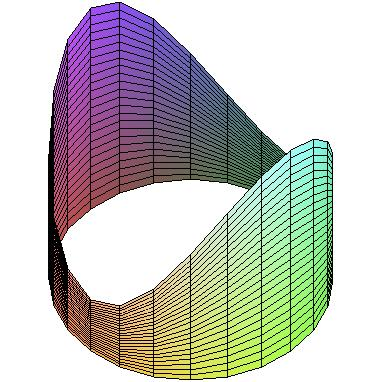
\includegraphics[width=\marginparwidth]{06-LineIntegrals/support/sheet-2}}%
 To find the area of a sheet of metal above the unit circle with
  height given by $f=x^2+4y^2$, first parametrize the curve $C\colon \vec
  r(t) = \langle\cos t,\sin t\rangle$, $0\leq t\leq 2\pi$. Then compute $A = \int_C f\,ds =
  \int_0^{2\pi} ((\cos t)^2 + 4 (\sin t)^2) \,|\langle-\sin t,\cos t\rangle|\,dt =
  \int_0^{2\pi} (\cos^2 t + 4 \sin^2 t) (1)\,dt$. To solve this integral,
  we can use integration tables, technology, or the trig identities
  $\cos^2 t= \frac{1+\cos 2t}{2}$ and $\sin^2 t = \frac{1-\cos
    2t}{2}$. This gives $$\int_0^{2\pi} \frac{1+\cos 2t}{2} +4 \frac{1-\cos
    2t}{2}dt = \int_0^{2\pi} \frac{5}{2} - \frac{3\cos 2t}{2}dt =
  \left.\left(\frac{5}{2}t - \frac{3\sin 2t}{4}\right)\right|_0^{2\pi} = 5\pi.$$
\end{example}

\begin{example}
\marginpartop{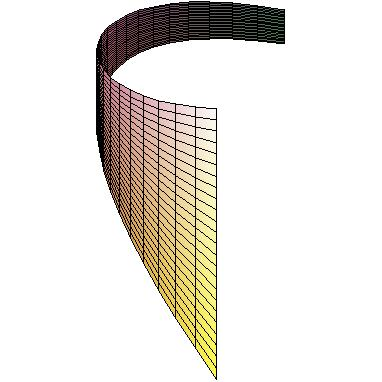
\includegraphics[width=\marginparwidth]{06-LineIntegrals/support/sheet-1}}%
The area of a sheet of metal above the curve $\vec
r(t)=\langle t,t^2\rangle$ for $-1<t<2$, with height given by
{$f=(x+2)(y+2)$}, is 
$\int_{-1}^{2}(t+2)(t^2+2)\sqrt{(1)^2+(2t)^2}\,dt 
= \int_{-1}^{2} (t+2)(t^2+2)\sqrt{1+4t^2}\,dt$. Solving this integral is
rather time consuming, and technology will quickly get an answer.
\end{example}


Please spend some time sharpening your integration skills (in
particular $u$ substitution and integration by parts), but do not
spend so much time doing complex integrals that you do not get to
practice the new ideas.


\section{Physical Applications}
We now develop average value, centroid, mass, center of mass, moment
of inertia, and radius of gyration. There are examples at the end of
this section of how to do all of this, as well as a ``Short Version''
which summarizes the ideas found herein. I strongly suggest you read
all of this at least once. It is okay if it doesn't all make sense
before discussion in class.  Reading it will help you understand, as
well as help you learn to read more complex mathematical ideas. 

\subsection{Averaging infinitely many things}

The average of a finite number of values is $y_1,\ldots,y_n$ is
$\frac{1}{n}\sum_{i=1}^n y_i$. To extend this to an infinite average
value, we use ``weighted averages.'' If a value $y$ occurs more than
once in a list of numbers to be averaged, let $y_1,\ldots,y_n$ be the
distinct values to be averaged and $c_i$ be the number of times $y_i$
occurred. The total number of values to be averaged is $C=\sum_{i=1}^n
c_i$ and the average of these values is $\frac{1}{C}\sum_{i=1}^n c_iy_i =
\sum_{i=1}^n \frac{c_i}{C}y_i = \sum_{i=1}^n w_i y_i$. The number
$w_i=\frac{c_i}{C}$ is called a weight corresponding to $y_i$, and it
represents the proportion of times $y_i$ occurs in the total number of
values. 

\begin{example}
 The average of $1,1,3,4,4,4,4$ can be computed by
  considering the three distinct values $y_1=1, y_2=3, y_3=4$ which
  occur with frequency $c_1=2, c_2=1, c_3=4$. The number of values is
  $C=c_1+c_2+c_3=7$ and the weights are
  $w_1=\frac{2}{7},w_2=\frac{1}{7},w_3=\frac{4}{7}$.  The average of
  these values is $\sum_{i=1}^3 w_i y_i =
  \frac{2}{7}(1)+\frac{1}{7}(3)+\frac{4}{7}(4) = 3$.

\end{example}

Much more could be
said about weighted averages and their importance in mathematics and
practical applications. The sum of the weights $w_i$ is always 1
because each weight represents a portion of the total, and adding up
all these portions gives 100\% of the total.

\subsubsection{Average value by using weighted averages}
The average value of a function is an extension of finite averages to
an infinite average of the output values of the function. Consider a
function $f(x,y,z)$ which represents the temperature at any point
$(x,y,z)$ in space. If a particle travels along the space curve given
by $C\colon\vec r (t)=\langle x,y,z\rangle$ for $a\leq t\leq b$, the average value
of $f$ along this space curve will be an average of the infinitely
many temperature values along $C$. Divide $C$ into tiny portions (by
dividing the interval $(a,b)$ up into many pieces
$a=t_0<t_1<t_2<\cdots<t_{n-1}<t_n=b$) and pick a representative point 
 $\vec r(t_k)$ for each portion of the curve. Assuming the heat
$f$ is continuous, the heat 
$f_{i}=f(\vec r(t_i))$ at this representative point 
is approximately the same as the heat $f$ for every point $\vec r(t)$
on the curve for $t_{k-1}\leq t\leq t_{k}$. If each portion of the curve has
length $\Delta s_i$, then the proportion of the total length located in the
$i$th bit of curve is $\frac{\Delta s_{i}}{s}$, where $s$ is the arc length
of $C$. We use this proportion as our weight in a weighted average
because it gives the proportion of times a heat $f$ value would occur
even in an infinite setting. The weighted average of $f_{i}$ using the
weights $w_{i}=\frac{\Delta s_{i}}{s}$ is approximately the average value
of $f$, 
$AV\approx \sum_{i=1}^n \frac{\Delta s_{i}}{s}f(\vec r(t_i)) 
= \frac{1}{s} \sum_{i=1}^n f(\vec r(t_i)) \Delta s_{i}$. As $\Delta s_{i}$
approaches zero, we obtain the integral formula $AV=\frac{1}{s}\int_C
f(\vec r(t))\,ds$. Often people will just write $AV=\frac{1}{s}\int_C f
\,ds$, where it is implied that you replace $x,y,z$ with what they are
in terms of $t$.  Remember that $ds = |\vec r\vp(t)|dt$. 

\subsubsection{Average Value by finding a constant that can be used to
replace $f$}
If we multiply both sides of the formula $AV=\frac{1}{s}\int_C f \,ds$ by
arc length $s$, then we obtain the formula $(AV)(s) = \int_C f \,ds$, or
$(AV)\int_C 1 \,ds = \int_C f \,ds$. Since $AV$ is a constant, bring it inside
the integral giving $\int_C (AV) \,ds = \int_C f \,ds$.  The last formula has a
geometric interpretation: average value ($AV$) is a constant value
such that if you replaced the integrand $f(x,y,z)$ with $AV$, then you
would obtain the same line integral. The formula used in previous calculus classes is
$AV (b-a) =\int_a^b f(x)dx$. The area underneath $f$ from $a$ to $b$ is
given by $\int_a^b f(x)dx$. Average value is the height $AV$ of a
rectangle with the same width which has the same area as the area
under $f$.  If you were to take an ant farm where the top of the sand
was given by the function and shake it so that the sand all leveled
off, then the height of the sand when you were done shaking would be
the average value.  

\bigskip

We have purposefully discussed average value in two different ways:
(1) using weighted averages, (2) replacing $f$ with $AV$ in the
formula $\int_C (AV) \,ds = \int_C f \,ds$ and solving for $AV$ which gives
$AV=\frac{1}{s}\int_C f \,ds$.  These two ideas will be used in the
applications which follow. 

\subsection{Centroid}
The centroid $(\bar x,\bar y,\bar z)$ of an object is the point in
space whose {$x,y,z$}-values are the average {$x,y,z$}-values.  The
average value formula gives $\bar x = \frac{1}{s}\int_C x\,ds, \bar y =
\frac{1}{s}\int_C y\,ds, \bar z = \frac{1}{s}\int_C z\,ds$, which when written
in vector form is equivalent to $ \langle\bar x,\bar y,\bar z\rangle =
\frac{1}{s}\int_C  \langle x,y,z\rangle \,ds$. In terms of weighted averages,
the weight attached to each point is $\frac{ds}{s}$, the proportion of
arc length corresponding to each point.

\subsection{Density and Mass}
\prepproblems{15.2: 23}%
A density is the measure of a quantity per unit something. The
derivative $\frac{dy}{dx}$ is a measure of change in $y$ per unit
change in $x$. A change $dy$ of a function for some given change $dx$
is computed by multiplying the density $\frac{dy}{dx}$ by the change
$dx$, giving us the familiar equation $dy = \frac{dy}{dx}dx$. Adding
up these approximate changes in $y$ gives the integral formula $\int_a^b
dy = \int_a^b f' dx$ which measures the total change in $y$ from $a$ to
$b$ (or more commonly called the fundamental theorem of calculus). 
Hopefully this was a review. The new idea is that density is the
measure of a quantity per unit something.

Mass density $\delta(x,y,z)$ in space is a measure of mass per unit volume,
i.e $\text{density}=\frac{\text{mass}}{\text{unit volume}}$. The
(mass) density of water is found by calculating the mass of some
quantity of water and dividing by its volume. The metric unit system
was created so that 1 kg of water occupies 1 liter of space, giving a
density of 1kg/L (this is how we connect mass and volume). Different
substances have different densities.  If you mix oil and water, the
density of oil is less than water which is why the oil and water
separate themselves with the oil on top and the water underneath.
When an object is made out of many different materials, the density of
the object may differ depending on where in the object you are.  This
is why we write $\delta(x,y,z)$, to reinforce the idea that density may
vary based upon which portion of the object you are considering.  To
find the mass of an object with constant density, we just multiply the
density by its volume.

If we consider an object that is located in space along a space curve
$C\colon\vec r (t)=\langle x,y,z\rangle$ for $a\leq t\leq b$, then it is more
convenient to think of density as mass per unit arc length.  This
gives us a density $\delta(x,y,z)$ at each point on the curve, and then the
mass of each little portion of the curve can then be approximated by
multiplying the density of one point of the piece by the length of
each little piece.

The density  (mass per unit length) at a point is the mass that would
result if points with the same density were to occupy 1 unit of arc
length. If points of density $\delta(x,y,z)$ occupied a curve of length $\Delta
s$, then the mass of that curve would be $\Delta m = \delta(x,y,z)\Delta s$. (Do you
see an integral formula coming? If so, try to write it down before you
read any more.) If we know the density of an object $\delta(x,y,z)$ for 
all $(x,y,z)$ along a curve $C\colon\vec r(t)$, then divide the curve $C$
into little arcs $\Delta s_{i}$. Approximate the mass of each arc by
assuming the density is constant on each little piece, which gives $\Delta
m_{i} \approx \delta(x_i,y_i,z_i)\Delta s_{i}$. Total mass is found by adding up these
little bits of mass, and then taking a limit as $\Delta s_{i}\to 0$, which
gives $m=\int_C \delta \,ds$.  In differential notation, we write $dm = \delta ds$,
 so $m=\int_C dm$ (mass is found by adding up little bits of mass).  

\subsection{Center of Mass and First Moments}
The center of mass of an object is the weighted average of the
$(x,y,z)$ values where the weights are given by the proportion of mass
$\frac{dm}{m}$ corresponding to each region. The integral formula is
$\langle\bar x,\bar y,\bar z\rangle = \frac{1}{m}\int_C
\langle x,y,z\rangle dm = \frac{1}{m}\int_C \langle x,y,z\rangle dm$. The
difference between center of mass and centroid is that for a centroid,
we assume $\delta$ is constant, so it comes out of the integral and cancels to give $\frac 1 s \int_C \langle x,y,z\rangle\,ds$.  

\subsubsection{First Moments of mass}
The quantities $M_{yz}=\int_C x dm, M_{xz}=\int_C y dm$, and  $M_{xy}=\int_C z
dm$ which appear in the formula for center of mass are called the
first moments of mass about the $yz$ plane, about the $xz$ plane, and
about the $xy$ plane, respectively. These first moments of mass are a
weighted directed measure of distance from a plane. 
To find the first moment about the plane $x=c$, we note that the
distance to the plane $x=c$ is $x-c$, so the moment is $M_{x=c}=\int_C
(x-c)dm$.  The center of mass is the value $\bar x$ such that the
moment about the plane $x=\bar x$ is zero, or $\int_C(x-\bar x)dm = 0$.
Since $\bar x$ is a constant, this becomes $0=\int_C x dm - \bar x \int_C dm$
or $\bar x m = \int x dm=M_{yz}=M_{x=0}$. Hence center of mass can be
written in terms of moments by the formulas
$\bar x =M_{yz}/m,\bar y =M_{xz}/m, \bar z = M_{xy}/m$. 
There are various applications of moments in statistics, physics, and
mathematics, however the language used in each field is slightly
different. Wikipedia has a wealth of information about this topic.

\subsection{Inertia}
\prepproblems{15.2: 71}%
Kinetic energy of a moving object is $\displaystyle KE=\frac{1}{2}
mv^2$, where $m$ is the mass and $v$ is the velocity. Imagine a
particle moving in a circular path of radius $r$ about some axis.  Let
$\theta(t)$ be the angle the particle is at at time $t$.  The net distance
the particle travels between times $t_1$ and $t_2$ is
$r\theta(t_2)-r\theta(t_1)$, so $r\theta(t)$ is the position function of the
particle.  The velocity is {$ v=\frac{d}{dt}(r\theta)=r\frac{d\theta}{dt} =
  r\omega(t) $}, where we call $\omega(t)$ the rotational velocity at time
$t$. The kinetic energy of a rotating particle is thus {$\displaystyle
  KE=\frac{1}{2} m(r\omega)^2 = \frac{1}{2} m r^2\omega^2$}. Since an object
which is rotating has particles at different radii, finding the total
kinetic energy of a rotating object requires more work.  We divide the
object into little pieces with mass {$\Delta m$} and rotate each little
piece around the axis of rotation, giving {$\displaystyle \Delta KE=
  \frac{1}{2} \Delta m r^2 \omega^2$}.  Summing gives us {$\displaystyle KE \approx \sum
  \frac{1}{2} \Delta m r^2 \omega^2 = \frac{1}{2} \omega^2 \sum r^2 \Delta m$}. Taking a
limit gives {$\displaystyle KE = \frac{1}{2} \omega^2 \int r^2 dm$}, where
{$r$} is the radius of rotation of a small piece of mass $dm$.  The
quantity {$I=\int r^2 dm$} is called a moment of inertia about an axis of
rotation (or a second moment). We can then write kinetic energy as
$KE=\frac{1}{2}v^2 m = \frac{1}{2}\omega^2 I$. Notice that a moment of
inertia takes the place of mass in rotational kinetic energy.

In 3D, the radius of rotation about an axis is the distance to the
axis.  The radius of rotation about the $x$-axis is $\sqrt{y^2+z^2}$,
the radius of rotation about the $y$-axis is $\sqrt{x^2+z^2}$, and the
radius of rotation about the $z$-axis is $\sqrt{x^2+y^2}$ (just leave
off $x$ when finding distance to $x$ axis, leave off $y$ when finding
distance to $y$-axis, and leave off $z$ when finding distance to $z$
axis). This gives the formulas for the moments of inertia for a curve
$C$ with density $\delta$ to be $I_x = \int_C (y^2+z^2)\delta \,ds$, $I_y = \int_C
(x^2+z^2)\delta \,ds$, and $I_z = \int_C (x^2+y^2)\delta \,ds$ (we squared each
distance, hence the square roots disappear).  The single formula $I=\int
r^2 dm$ describes all of these formulas. You can find the moment of
inertia about any line. All you have to do is find a formula for the
distance from a point on the curve to the axis of rotation.

\subsubsection{Radii of Gyration}

The radius of gyration $R$ about an axis is a positive radius $R$ such
that if we replace $r^2$ with $R^2$ in the moment of inertia equation,
we would have $\int R^2 dm = \int r^2 dm$. This means $R^2 m = I$ or
$R=\sqrt{I/m}$. The radius of gyration about the $x$-axis is $R_x =
\sqrt{I_x/m}$, and similarly $R_y = \sqrt{I_y/m}$ and $R_z=
\sqrt{I_z/m}$. The radius of gyration about an axis is a rotational
center of mass. It is used in studying energy, and is often used to
simplify complex problems. This derivation was similar to us finding
the center of mass, where we replaced $x$ with $\bar x$ to obtain the
equality $\int \bar x dm = \int x dm$ or $\bar x =(\int x dm)/m$.

\subsection{Summary}
Most everything we learned above is summarized below in differential
notation.  Essentially, in this unit, you are learning to
use and derive differential formulas to find quantities such as area,
centroids, mass, center of mass, moments, moments of
inertia, and radii of gyration.  Let $C\colon r(t)$ be a curve.
\begin{itemize}
\item Area: $dA = fdx$ for an interval, $dA=fds $ for a curve.
\item Average Value: $(AV) s = \int f \,ds$, so $AV=\frac 1 s \int f\,ds$.
\item Centroid: $\langle\bar x,\bar y,\bar z\rangle s =\int
\langle x,y,z\rangle\, ds$, so $\langle\bar x,\bar y,\bar z\rangle= \frac 1 s \int \langle x,y,z\rangle\,ds$ (find average $x,y,z$ values)
\item Mass: $dm = \delta ds $, where $\delta$ is a function giving the density at a point.
\item Center of Mass: Just replace $s$ with $m$ in centroid,
$\langle\bar x,\bar y,\bar z\rangle m = \int_C \langle x,y,z\rangle dm$,
where $M_{yz}=\int_C \bar x dm = \int x dm$ is a first moment of mass, so $\bar x = M_{yz}/m$.  Similarly for $M_{xz}$ and $M_{xy}$.
\item $I = \int r^2 dm$ is a moment of inertia, and $\int R^2 dm = \int r^2 dm$
gives $R^2 m =I$ or $R=\sqrt{I/m}$ as the radius of gyration (where
$r$ represents the generic distance from a point in space to the axis
of rotation).
\end{itemize}
I strongly suggest that you start each problem from a differential
formula, and then work from there to convert it to a line integral in
terms of t that you can evaluate.  This practice will make parts of
the next two units much easier.


\subsection{Big Example}
\prepproblems{Make up your own curve and density function and calculate
  all of these quantities}%
Here is an example of each idea with a single curve. When you create
your lesson plan, I suggest that you focus on one particular space
curve, density, and function.  Then show how all the formulas are
developed from there.

Consider the elliptical helix $C\colon\vec r (t) = \langle3\sin t, 4\cos t,
t\rangle$ for $0\leq t\leq 2\pi$.  The arc length differential is $$ds = |\vec
r\vp(t)|dt = \sqrt{(3\cos t)^2 + (-4\sin t)^2+1^2}dt = \sqrt{9\cos^2
t+16\sin^2 t+1}dt.$$ Arc length is then  $$s=\int_C ds =
\int_{0}^{2\pi}\sqrt{9\cos^2 t+16\sin^2 t+1}dt.$$

The centroid of this curve is found using the integral formulas (which
are too ugly to bother solving by hand):
\begin{align*}
\bar x &= \frac{\int_C x ds}{\int_C ds} = \frac{\int_{0}^{2\pi}(3\sin
t)\sqrt{9\cos^2 t+16\sin^2 t+1}\,dt}{\int_{0}^{2\pi}\sqrt{9\cos^2 t+16\sin^2
t+1}\,dt}\\
\bar y &= \frac{\int_C y ds}{\int_C ds} = \frac{\int_{0}^{2\pi}(4\cos
t)\sqrt{9\cos^2 t+16\sin^2 t+1}\,dt}{\int_{0}^{2\pi}\sqrt{9\cos^2 t+16\sin^2
t+1}\,dt}\\
\bar z &= \frac{\int_C z ds}{\int_C ds} = \frac{\int_{0}^{2\pi}(t)\sqrt{9\cos^2
t+16\sin^2 t+1}\,dt}{\int_{0}^{2\pi}\sqrt{9\cos^2 t+16\sin^2 t+1}\,dt}
\end{align*}
or you can use the single vector formula (which means compute the
three integrals above) 
$$\langle\bar x,\bar y,\bar z\rangle = \frac{\int_C \langle x,y,z\rangle
ds}{\int_C ds} = \frac{\int_{0}^{2\pi} \langle3\sin t, 4\cos t,
t\rangle\sqrt{9\cos^2 t+16\sin^2 t+1}\,dt}{\int_{0}^{2\pi}\sqrt{9\cos^2
t+16\sin^2 t+1}\,dt}$$

If the curve represents a wire in space with density given by $\delta
(x,y,z) = x^2+y^2z$ kg/L, then $dm = \delta ds$, and we can calculate the
centroid as follows (just replace $ds$ in the above formulas with
$dm=\delta ds$):
\begin{align*}
m=&\int dm = \int_C \delta ds = \int_{0}^{2\pi}((3\sin t)^2+(4\cos
t)^2(t))\sqrt{9\cos^2 t+16\sin^2 t+1}\,dt\\
\bar x &= \frac{\int x dm}{\int dm}= \frac{\int_C x \delta ds}{\int_C \delta ds} =
\frac{\int_{0}^{2\pi}(3\sin t)((3\sin t)^2+(4\cos t)^2(t))\sqrt{9\cos^2
t+16\sin^2 t+1}\,dt}{\int_{0}^{2\pi}((3\sin t)^2+(4\cos t)^2(t))\sqrt{9\cos^2
t+16\sin^2 t+1}\,dt}\\
\bar y &= \frac{\int y dm}{\int dm}= \frac{\int_C y \delta ds}{\int_C \delta ds} =
\frac{\int_{0}^{2\pi}(4\cos t)((3\sin t)^2+(4\cos t)^2(t))\sqrt{9\cos^2
t+16\sin^2 t+1}\,dt}{\int_{0}^{2\pi}((3\sin t)^2+(4\cos t)^2(t))\sqrt{9\cos^2
t+16\sin^2 t+1}\,dt}\\
\bar z &= \frac{\int z dm}{\int dm}= \frac{\int_C z \delta ds}{\int_C \delta ds} =
\frac{\int_{0}^{2\pi}(t)((3\sin t)^2+(4\cos t)^2(t))\sqrt{9\cos^2
t+16\sin^2 t+1}\,dt}{\int_{0}^{2\pi}((3\sin t)^2+(4\cos t)^2(t))\sqrt{9\cos^2
t+16\sin^2 t+1}\,dt}
\end{align*}
The first moments of mass, second moments of inertia, and radii of
gyration are given by:
\begin{align*}
M_{yz} &= \int x dm = \int_C x \delta ds = \int_{0}^{2\pi}(3\sin t)((3\sin t)^2+(4\cos
t)^2(t))\sqrt{9\cos^2 t+16\sin^2 t+1}\,dt\\
M_{xz} &= \int y dm = \int_C y \delta ds = \int_{0}^{2\pi}(4\cos t)((3\sin t)^2+(4\cos
t)^2(t))\sqrt{9\cos^2 t+16\sin^2 t+1}\,dt\\
M_{xy} &= \int z dm = \int_C z \delta ds = \int_{0}^{2\pi}(t)((3\sin t)^2+(4\cos
t)^2(t))\sqrt{9\cos^2 t+16\sin^2 t+1}\,dt\\
I_x &= \int r^2 dm =\int y^2+z^2 dm =\int_{0}^{2\pi}[(4\cos t)^2+(t)^2]((3\sin
t)^2+(4\cos t)^2(t))\sqrt{9\cos^2 t+16\sin^2 t+1}\,dt\\
I_y &= \int r^2 dm =\int x^2+z^2 dm =\int_{0}^{2\pi}[(3\sin t)^2+(t)^2]((3\sin
t)^2+(4\cos t)^2(t))\sqrt{9\cos^2 t+16\sin^2 t+1}\,dt\\
I_z &= \int r^2 dm =\int x^2+y^2 dm =\int_{0}^{2\pi}[(3\sin t)^2+(4\cos
t)^2]((3\sin t)^2+(4\cos t)^2(t))\sqrt{9\cos^2 t+16\sin^2 t+1}\,dt\\
&R_x=\sqrt{I_x/m},\
R_y=\sqrt{I_y/m},\
R_z=\sqrt{I_z/m},\
\end{align*}





%%% Local Variables: 
%%% mode: latex
%%% TeX-master: "../multivariable-calculus"
%%% End: 






\newgeometry{left=1in,right=1in,top=1in,bottom=1in}
\newpage

\section{Preparation}

\subsection{Lesson Plans}

This chapter covers the following ideas. When you create your lesson plan, it should contain examples which illustrate these key ideas. Before you take the quiz on this unit, meet with another student out of class and teach each other from the examples on your lesson plan. 

% A list of objectives for the chapter
%\begin{enumerate}
%\item ...
%\end{enumerate}

\begin{enumerate}
\item Describe how to integrate a function along a curve. Use line
  integrals to find the area of a sheet of metal with height
  $z=f(x,y)$ above a curve $\vec r(t)=\langle x(t),y(t)\rangle$ and the average
  value of a function along a curve.
\item Find the following geometric properties of a curve: centroid,
  mass, center of mass, moments of mass, moments of inertia, and radii
  of gyration.
\end{enumerate}

%%% Local Variables: 
%%% mode: latex
%%% TeX-master: "../multivariable-calculus"
%%% End: 
%$


%\subsection{Preparation Problems}

%Here are the preparation problems for this unit.

\subsection{Homework}

In the following list, the ``basic practice'' problems should be quick
problems to help you master the ideas.  The ``good problems'' will
require a little more work.  The theory and application problems are
ones that will challenge you more; make sure you do the problems from
this area to fully master the material.  

{\noindent %\footnotesize 
\begin{tabular}{|l|c|l|l|l|l|}\hline
Topic &Sec &Basic Practice &Good Problems &Thy/App \\\hline
Vector Fields & 15.1&21--30,35--42,51--56 & 31--34& \\\hline
Line Integrals & 15.2&1--18,21--32,35--40, 61--68 & 19--20, 33--34, 43--60, 79--80 & 41--42, 69--76, 81--85\\\hline
Independence of Path & 15.3&1--36 & 37--39& 43--53\\\hline
\end{tabular}

}



%%% Local Variables: 
%%% mode: latex
%%% TeX-master: "../multivariable-calculus"
%%% End: 


%%% Local Variables: 
%%% mode: latex
%%% TeX-master: "../multivariable-calculus"
%%% End: 

\restoregeometry



\chapter{Line Integrals in Vector Fields}

This chapter covers the following ideas. 

% A list of objectives for the chapter
%\begin{enumerate}
%\item ...
%\end{enumerate}

\begin{enumerate}
\item Compute work done by a non-constant force $\vec F$ along a
  non-straight curve $C\colon\vec r(t)$.
\item Define and compute flow and circulation along a curve using the
  ideas from computing work.  Be able to compute flow along piecewise
  smooth curves. Give an application of flow in terms of fluid flow.
\item Compute the flux in the plane of a vector field $\vec F$ across
  a smooth curve $C\colon\vec r(t) = \langle x(t),y(t)\rangle$.  Give an
  application of flux in terms of fluid flow.
\item Be able to draw vector fields and determine if a given field is a
  gradient field (hence conservative)
\item Use the fundamental theorem of line integrals to greatly
  simplify work calculations.
\end{enumerate}

%%% Local Variables: 
%%% mode: latex
%%% TeX-master: "../multivariable-calculus"
%%% End: 
%$

\section{Work}

If a constant force $\vec F$ acts on an object through a displacement
in a straight line, then work is {$ W= \vec F\cdot \vec r $} (we use the
dot product).  If the displacement is not linear or the force is not
constant, then this formula breaks down. To find work done by a
non-constant force $\vec F$ along an arbitrary curve $\vec r$, start
by breaking the curve up into little pieces $\Delta \vec r = \vec T \Delta s$
(direction times magnitude, where $\vec T$ is the unit tangent
vector). On each little piece of the curve, the force is approximately
constant, and the displacement is approximately a straight line, so we
approximate the work done on each little piece as {$ \Delta W \approx \vec F \cdot \Delta
\vec r = \vec F \cdot \vec T \Delta s $}.  Sum the little pieces of work to get an
approximate total work {$ W \approx \sum \vec F \cdot \vec T \Delta s $}.  Taking limits
gives 
$$%\displaystyle
W = \int_C \vec F\cdot \vec T \,ds 
= \int_a^b\vec F\cdot \frac{\vec r\vp}{|\vec r\vp|}|\vec r\vp| dt 
= \int_a^b\vec F\cdot \vec r\vp dt 
= \int_C \vec F\cdot d\vec r.$$
(We use the differential notation {$ d\vec r= \vec r\vp dt $}, which
comes from the equation {$ \frac{d\vec r}{dt} = \vec r\vp $}.)
If {$ \vec F = \langle M,N,P\rangle $} for some functions $M,N$, and
$P$, then the work can be written 
$$W = \int_C \langle M,N,P\rangle\cdot\langle dx,dy,dz\rangle 
= \int_C Mdx+Ndy+Pdz.$$ These many formulas are different ways of
representing the exact same quantity.

\subsection{Flow (synonym for work) and Circulation (work on a closed
curve)}
Flow along a curve $C$ is a measure of how much fluid (with velocity
field {$ \vec F = \langle M,N,P\rangle $}) flows along a curve {$C\colon \vec r(t)$ , $a\leq
  t\leq b$,} per unit time. This quantity is particularly useful in the
study of fluid mechanics, for example, studying how air flow near a
wing provides lift for an airplane. The component of the velocity in
the direction of the curve is the scalar projection $|\proj_{\vec
  T}\vec F| = \vec F\cdot \vec T$.  For each little piece of curve $ds$,
the product $\vec F\cdot \vec T ds$ is approximately how much fluid will
flow along this portion of the curve.  Summing these small bits of
flow gives the total flow by the line integral {$\int_C \vec F\cdot \vec T
  \,ds = \int_C \vec F\cdot d\vec r = \int_C Mdx+Ndy+Pdz $}. If the curve is a
simple closed curve (meaning it is piecewise smooth, starts and ends
at the same point, and does not cross itself), then flow along $C$ is
called circulation around $C$.  We sometimes add a closed circle to
the integral to emphasize this, as in {$ \oint_C \vec F \cdot d\vec r $}. 

The only difference between work, flow, and circulation is how we
interpret the vector field.  The computations are the same.


% A vector field is said to be
% \textbf{conservative} if circulation along every closed loop is zero,
% or equivalently if work calculations are independent of the path,
% i.e., only depend on starting and ending points.


\begin{example}
\marginpartop{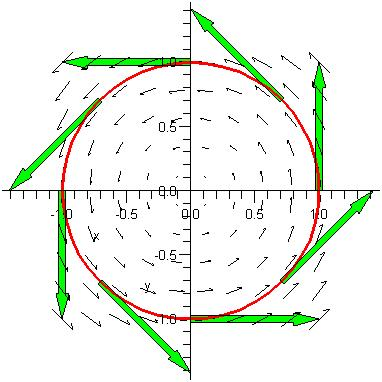
\includegraphics[width=\marginparwidth]{07-GradientFields/support/work-1}}%
Consider the vector field {$\vec F(x,y)=\langle-y,x\rangle$}.
The circulation of {$\vec F$} along a circle of radius $a$ that is
traversed counter-clockwise is found by first parametrizing the circle
$C\colon r(t) = \langle a\cos t,a\sin t\rangle$, $0\leq t\leq2\pi$ (so that we traverse it
counter-clockwise). Hence $\vec r\vp(t) = \langle-a\sin t,a\cos t\rangle$ and
$\int_C\vec F\cdot d\vec r = \int_0^{2\pi} \langle-y,x\rangle\cdot \langle-a\sin t,a\cos t\rangle dt =
\int_0^{2\pi} \langle-a\sin t,a\cos t\rangle\cdot \langle-a\sin t,a\cos t\rangle dt = \int_0^{2\pi}
a^2\sin^2 t+a^2\cos^2 t dt = \int_0^{2\pi} a^2 dt = 2\pi a^2$.  Notice that
the integral of a constant along an interval is always the length of
the interval multiplied by that constant.  This will speed up the
calculation of many integrals that we encounter throughout the
semester.
\end{example}

\begin{example}
\marginpartop{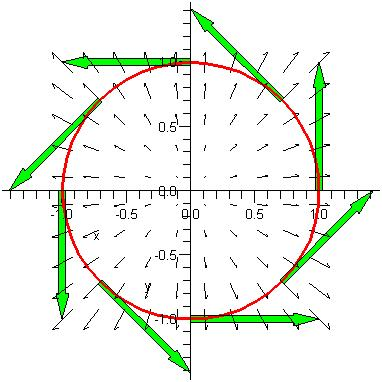
\includegraphics[width=\marginparwidth]{07-GradientFields/support/work-2}}%
Now consider the vector field {$\vec F(x,y)=\langle x,y\rangle$}.  To calculate
  the circulation of {$\vec F$} along a circle of radius $a$, we use
  the same parametrization as last time. This time using the formula
  $\int_C Mdx+Ndy$, we have $x=a\cos t$, $y=a\sin t$, $dx=-a\sin t$,
  $dy=a\cos t$, $M=x=a\cos t$, and $N=y=a\sin t$, so $\int_C Mdx+Ndy =
  \int_0^{2\pi} a\cos t (-a\sin t) + a \sin t (a\cos t) dt = \int_0^{2\pi} 0 dt
  = 0$.  Notice that the vector field is always orthogonal to the unit
  tangent vector, which is why the flow along $C$ is zero.
\end{example}

\begin{example}
\marginpartop{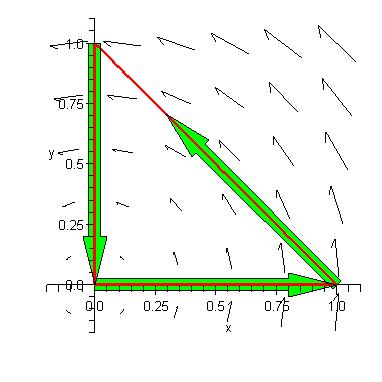
\includegraphics[width=\marginparwidth]{07-GradientFields/support/work-3}}%
Now consider the vector field {$\vec
  F(x,y)=\langle-y,x\rangle$} and the curve which forms the boundary of the
triangle with vertices $(0,0), (1,0), (0,1)$ and goes around
counter-clockwise. To find the work done by $\vec F$ through the
displacement along $C$ counter-clockwise (or the flow along $C$, or the circulation
around $C$), we first have to parametrize the curve.  This is a
piecewise smooth curve and, as such, is parametrized using 3 different
curves.  From (0,0) to (1,0), we get a direction vector for the line
segment by subtracting the points: $\langle1-0,0-0\rangle$. We then write
$C_1\colon\vec r_1(t) = \langle1,0\rangle t+\langle0,0\rangle$ for $0\leq t \leq 1$ (we know to stop at
1, because $\vec r_1(1)=\langle1,0\rangle$).  Similarly for the segment from (1,0)
to (0,1), we write $C_2\colon\vec r_2(t) = \langle-1,1\rangle t+\langle1,0\rangle$ for $0\leq t \leq
1$. For the segment from (0,1) to (0,0), we write $C_3\colon\vec r_3(t) =
\langle0,-1\rangle t+\langle0,1\rangle$ for $0\leq t \leq 1$. We then compute
\begin{alignat*}{3}
  &\oint_C \vec F\cdot d\vec r \\
  &= \int_{C_1} \vec F\cdot d\vec r_1 &&+ \int_{C_2} \vec F\cdot d\vec r_2 &&+ \int_{C_3}
  \vec F\cdot d\vec r_3\\
  &= \int_0^1 \langle-y,x\rangle\cdot \langle1,0\rangle dt &&+ \int_0^1
  \langle-y,x\rangle\cdot \langle-1,1\rangle dt &&+ \int_0^1 \langle-y,x\rangle\cdot
  \langle0,-1\rangle dt\\
  &= \int_0^1 \langle-(0),(t+0)\rangle\cdot \langle1,0\rangle dt &&+ \int_0^1
  \langle-(t+0),(1-t)\rangle\cdot \langle-1,1\rangle dt &&+ \int_0^1
  \langle-(1-t),0\rangle\cdot \langle0,-1\rangle dt\\
  &= \int_0^1 0 dt &&+ \int_0^1 (t+0)+(1-t)dt &&+ \int_0^1 0 dt\\
  &= 0 &&+ 1 &&+ 0 \\
  &= 1.
\end{alignat*}
\end{example}

\section{Flux across a smooth curve} 

Any simple closed curve (piecewise smooth, doesn't cross itself, and
starts and ends at the same point) divides the plane into two regions,
which we will call the inside and outside of the curve. Just as flow
measures the rate at which fluid moves \emph{along} a curve, flux
measures the rate at which fluid moves \emph{across} a simple closed
curve.  By convention, if fluid is flowing out of the region, then there
is a positive flux across the curve which is the boundary of the
region. If you were to turn on a faucet at the origin and let water
flow onto the plane, the water would flow outwards, and the flux would
be positive across any curve which encircled the origin.
Alternatively, if you placed the drain of a sink at the origin, then
flux across a curve encircling the origin would be negative (i.e.,
water would be flowing into the region bounded by the curve).

In order to determine the flux across a curve, we need a vector
pointing out of the curve.  Let $\vec n$ be an outward-pointing unit
normal vector.  Then $\vec F\cdot \vec n$ is the component of $\vec F$ in
the outward normal direction. Break up the curve into small bits of
curve $ds$.  Then $d\text{Flux} = \vec F\cdot \vec n \,ds$ is the small
amount of fluid which flows across each small bit $ds$ of
curve. \textbf{For the following formula, we will assume that we are
  traversing the curve counter-clockwise.}  If {$\langle dx,dy\rangle$} represents
the tangential direction in the counter-clockwise direction, then {$\langle
  dy,-dx\rangle$} gives the direction of the outward-pointing normal (we can
see this since the dot product with the tangential vector is zero, and
the vector points outward). A unit outward normal vector is hence $
\frac{\langle dy,-dx\rangle}{\sqrt{dy^2+dx^2}}$. For flux across a curve $C$, we
add up the small bits of flux to get the formula 

\begin{align*}
  \text{Flux } &= \int_C\,d\text{Flux} = \int_C\vec F\cdot \vec n \,ds = \int_C\vec
  F\cdot \frac{\langle dy,-dx\rangle}{\sqrt{dy^2+dx^2}} \sqrt{dx^2+dy^2} \\
  &= \int_C \langle M,N\rangle
  \cdot <dy,-dx> = \int_C Mdy-Ndx.
\end{align*}
  In order to use this last formula, we
\emph{must} be traversing the curve in a counter-clockwise direction
(otherwise, $\langle dy,-dx\rangle$ won't be an outward-pointing normal vector).

\begin{example}
\marginpar{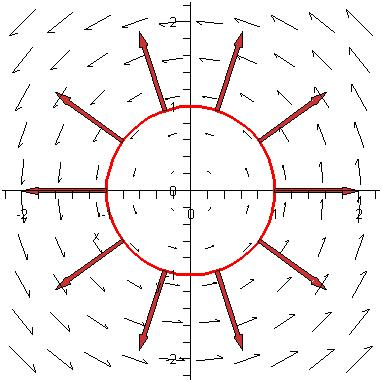
\includegraphics[width=\marginparwidth]{07-GradientFields/support/flux-1}}%
 Consider the vector field {$\vec F(x,y)=\langle-y,x\rangle$}.  The flux of
  {$\vec F$} across a circle of radius $a$ is found by first
  parametrizing the circle $C\colon r(t) = \langle a\cos t,a\sin t\rangle$.  Hence $\vec
  r\vp(t) = \langle-a\sin t,a\cos t\rangle$, or $dx=-a\sin t$ and $dy = a\cos
  t$. Hence we have $\int_C Mdy-Ndx = \int_0^{2\pi} (-a\sin t)(a\cos t)-(a\cos
  t)(-a\sin t)dt = \int_0^{2\pi} 0 dt = 0$.  In other words, no fluid is
  moving across the curve, in or out of the region.  Notice that this
  spin vector field is always orthogonal to the outward normal. This should
  visually show that the flux is zero. It is valuable to look at a
  picture and try to decide if the flux is zero, positive, or
  negative, as this will give you some intuition about flux.
\end{example}

\begin{example}
\marginpartop{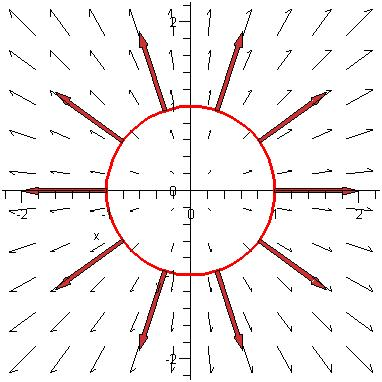
\includegraphics[width=\marginparwidth]{07-GradientFields/support/flux-2}}%
 Consider the vector field {$\vec F(x,y)=\langle x,y\rangle$}.  We use the same
  parametrization as the previous examples, so $x=a\cos t$, $y=a\sin t$,
  $dx=-a\sin t$, $dy=a\cos t$, $M=x=a\cos t$, and $N=y=a\sin t$. This gives the
  flux of $\vec F$ across $C$ as $\int_C Mdy-Ndx = \int_0^{2\pi} a\cos t
  (a\cos t) - a \sin t (-a\sin t) dt = \int_0^{2\pi} a^2(\cos^2t+\sin^2t)
  dt = 2\pi a^2$.  If our vector field is giving the velocity of water
  in meters per second, then this result says that $2\pi a^2$ square
  meters of water is flowing out of the circle per second.  You should
  notice that the vector field in this instance is always pointing out
  of the circle. Since the vector field and the outward normal are in
  the same direction, the flux is positive. Fluid is moving out of the
  interior of the circle.
\end{example}

\begin{example}
\marginpartop{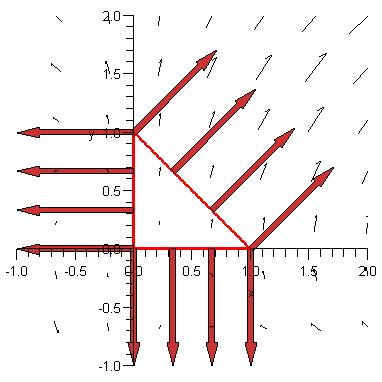
\includegraphics[width=\marginparwidth]{07-GradientFields/support/flux-3}}%
 Consider the vector field {$\vec F(x,y)=\langle xy,x+y\rangle$} and the curve $C$
  which forms the boundary of the triangle with vertices $(0,0),
  (1,0), (0,1)$. We first parametrize $C$ by finding a parametrization
  for each curve (remember: we need to traverse in a counter-clockwise
  direction to use our formula). This already done above, and we had
  the three curves $C_1\colon\vec r_1(t) = \langle1,0\rangle t+\langle0,0\rangle$ for $0\leq t \leq 1$,
  $C_2\colon\vec r_2(t) = \langle-1,1\rangle t+\langle1,0\rangle$ for $0\leq t \leq 1$, and $C_3\colon\vec
  r_3(t) = \langle0,-1\rangle t+\langle0,1\rangle$ for $0\leq t \leq 1$. We then compute the flux of
  $\vec F$ across $C$ as 
 \begin{alignat*}{3}
    &\oint_C Mdy-Ndx\\
    &= \int_{C_1}
    (M)(0) - (x+y)(1)dt &&+ \int_{C_2} (xy)(1)-(x+y)(-1)dt &&+
    \int_{C_3} (xy)(-1)-(N)(0)dt\\
    &= \int_0^1 - (t+0) dt &&+ \int_0^1 (1-t)(t)+(1-t)+(t) dt &&+ \int_0^1
    (0)(1-t)(-1) dt\\
    &= \int_0^1 - t dt &&+ \int_0^1 t-t^2 + 1  dt &&+ \int_0^1 0 dt\\
    &= -\frac{1}{2} &&+ \frac{1}{2}-\frac{1}{3}+1 &&+ 0 \\
    &= \frac{2}{3}
  \end{alignat*}

\end{example}


\section{Summary}
\label{sec:summary}

In summary, we've seen these new differentials.    Let $C\colon r(t)$ be a curve and
$F=\langle M,N,P\rangle$ be a vector field.
\begin{enumerate}
\item Work: $d\text{Work} = \vec F\cdot \vec T ds = \vec F\cdot d\vec r$, which is also written as $Mdx+Ndy$ (in 2D) and $Mdx+Ndy+Pdz$ (in 3D), where $\vec T$ is
a unit tangent vector to $C$.
\item Flux: $d\text{Flux} = \vec F\cdot \vec n ds = Mdy-Ndx$ where $\vec
n$ is a unit normal vector to $C$ and $C$ is traversed counter-clockwise.
\end{enumerate}

\section{Gradients, Potentials, and the Fundamental Theorem}

When the output dimension of a function is one, {i.e.,
  $f\colon{\mathbb{R}}^n\to {\mathbb{R}}^1$}, then the derivative is called
the \define{gradient} and is written in vector form as {$\nabla f = \langle f_x,f_y,f_z\rangle$}.
If a vector field {$\vec F = \langle M,N,P\rangle$} is the gradient of some
function {$f$} (so that {$\nabla f= \vec F$}), then we say that the vector
field {$\vec F$} is a \define{gradient field}, and the function {$f$} is called
a \define{potential} for {$\vec F$}. The potential of a gradient field appears
in differential equations, engineering, physics, and probably many
other places.

\subsection{Test for a gradient field}

If a vector field $\vec F$ is a gradient field (meaning there is an
$f$ such that $\nabla f=\vec F$), and the potential $f$ has continuous
second derivatives, then the second-order mixed partial derivatives
must be equal, namely $f_{xy}=f_{yx}$, $f_{xz}=f_{zx}$, and
$f_{yz}=f_{zy}$. So if $\vec F = \langle M,N,P\rangle$ is a gradient field and the
components of $\vec F$ have continous partial derivatives, then since
$M=f_x$, $N=f_y$, and $P=f_z$, we must have $M_y=N_x$, $M_z=P_x$, and
$N_z=P_y$. If these partial derivatives do not agree, then the vector
field cannot be a gradient field.  This gives us an easy way to
determine that a vector field is \emph{not} a gradient field.

\begin{example}
The vector field $\langle-y,x,-yx\rangle$ is not a
  gradient field because {$M_y=-1$} is not equal to {$N_x=1$}.
\end{example}
To prove a vector field does not have a potential, you must show that
either $M_x\neq N_y$, $M_z\neq P_x$, or $N_z\neq P_y$. It is insufficient to
say ``There is no potential because I could not find one.''


When $\vec F$ is defined on a ``nice'' set (which is true in many
situations in real life) and has continous partial derivatives, the check
works the other way as well.  For example, if a vector field $\vec
F=\langle M,N,P\rangle$ is defined on all of $\mathbb{R}^3$ (which is a ``nice''
set), $\vec F$ has continous partial derivatives, and $M_y=N_x$,
$M_z=P_x$, and $N_z=P_y$, then $\vec F$ is a gradient field (i.e.,
there is a potential function $f$ such that $\vec F = \nabla f$).  This
gives us a very nice way of checking if a vector field is a gradient
field.  See Section~\ref{sec:nice-sets} for a discussion of what a ``nice'' set is
and what happens when a vector field is not defined over a ``nice''
set.


\begin{example}
The vector field $\vec F=\langle x,z,y\rangle$ is
  a gradient field because $\vec F$ is defined on all of
  $\mathbb{R}^3$, each component has continous partial derivatives,
  and $M_y=0=N_x$, $M_z=0=P_x$, and $N_z=1=P_y$.  Notice that
  $f=x^2/2+yz$ gives $\nabla f = \langle x,z,y\rangle=\vec F$.
\end{example}

\begin{definition}[Exact differential forms]
A \define{differential form} is an
expression of the form {$Mdx+Ndy+Pdz$}.  On the other hand, if we have
a function $f(x,y,z)$, the differential of $f$ is 
$$df = Df d\vec x
= \begin{bmatrix}f_x&f_y&f_z
\end{bmatrix}\begin{bmatrix}dx\\dy\\dz\end{bmatrix}=f_x dx+f_y dy+f_z
dz.$$ If a differential form is actually the differential of a
function {$f$}, then the differential form is said to be
\define{exact}.  The function {$f$} is called a \define{potential} for the
differential form.  Notice that {$Mdx+Ndy+Pdz$} is exact if and only
if {$\vec F = \langle M,N,P\rangle$} is a gradient field.
\end{definition}

\begin{example}
The differential form $-ydx+xdy-yxdz$ is not
  exact since the field $\langle-y,x,-yx\rangle$ is not a gradient
  field (see above).  The differential form $xdx+zdy+ydz$ is exact
  since the field $\langle x,z,y\rangle$ is a gradient field (see
  above).
\end{example}
\subsection{Finding a potential (undoing a total derivative):} If we know
$\vec F=\langle M,N,P\rangle$ is a gradient field, then to find a potential
function $f$, we simultaneously solve the differential equations
$f_x=M$, $f_y=N$, and $f_z=P$.  In other words, we have to find a
function $f$ which is a solution of all three integrals $\int Mdx$, $\int
Ndy$, and $\int Pdz$.  Essentially, this is undoing the total
derivative. The following examples illustrate two methods of doing so.
The first method matches the book, while the second is quicker route which
simplifies the general idea.
\begin{example} Consider the vector field $\vec
F=\langle2xy+x,x^2-3z,-3y+z^2\rangle$. Since $D\vec F$ is continuous and
$M_y=2x=N_x$, $M_z=0=P_x$, and $N_z=-3=P_y$, the vector field $\vec F$ is a
gradient field, so $\vec F$ has a potential function $f$, and $f_x=M$,
$f_y=N$, and $f_z=P$.  To find $f$, we use two methods.

\textbf{Method 1:} In this method, we do several integrals, one after another.
\begin{enumerate}
\item Integrate $\int f_x\,dx=\int M\,dx$ to get $\int 2xy+x\,dx =
  x^2y+x^2/2+A(y,z)=f$, where $A$ is a constant with respect to $x$,
  which means that $A$ may actually be a function of $y$ and $z$.
\item Differentiate $f$ with respect to $y$ to obtain
  $N=f_y=\frac{\partial}{\partial y}[x^2y+x^2/2+A(y,z)] = x^2+A_y(y,z)$. Therefore,
  $x^2-3z=x^2+A_y(y,z)$, so $A_y(y,z)= -3z$ and $f_y=x^2-3z$.
\item Integrate $A_y$ with respect to $y$ to obtain $A(y,z)=\int -3z dy =
  -3yz+B(z)$, where $B$ is a constant with respect to $y$, which means
  that $B$ may actually be a function of $z$.  Thus,
  $f=x^2y+x^2/2-3yz+B(z)$.
\item Differentiate $f$ with respect to $z$ to get $P=f_z=-3y+B_z(z)$,
  so $-3y+z^2=-3y+B_z(z)$, so $B_z(z)=z^2$.
\item Integrate $B$ with respect to $z$ to get $B(z)=\int z^2 dz =
  z^3/3+C$ for some constant $C$ (and this is really a numeric
  constant!).  Hence a potential is $f= x^2y+x^2/2-3yz+z^3/3+C$ for
  any constant $C$.
\end{enumerate}

It is easy to check that $f$ is a potential by computing $\nabla f =
\langle2xy+x,x^2-3z,-3y+z^2\rangle$, which should equal $\vec F$.
Please, \emph{please} always check your answer by calculating $\nabla
f$ and making sure that it equals $\vec F$.

\textbf{Method 2:} As an alternative approach, integrate all three
functions simultaneously, ignoring the constants, to get $\int M dx =
x^2y+x^2/2$, $\int N dy = x^2y+-3yz$, and $\int P dz = -3yz +z^3/3$.
Provided a potential exists, then the function $f$ is formed by
summing these integrals, ignoring duplicated terms. Since $x^2y$ and
$-3yz$ appear in multiple integrals (are duplicated terms), we include
them once in the sum to obtain $f= x^2y+x^2/2-3yz+z^3/3$ as a
potential function. This method will work if a potential exists.
\end{example}

\begin{example}
  As another example, consider the
  vector field $\vec F(x,y,z) = \langle
  xy+yz+1,x^2/2+xz-3z,xy-3y\rangle$.  The test for a gradient field
  shows $M_y=x+z=N_x$, $M_z=y=P_x$, and $N_z=x-3=P_y$, which means
  that $\vec F$ is a gradient field.  A potential is found by
  integrating $\int xy+yz+1 dx = \frac12x^2y+xyz+x$, $\int x^2/2+xz-3z
  dy =\frac12x^2y+xyz-3yz$, and $\int xy-3y dz = xyz-3yz$. The term
  $xyz$ appears in all three results, $\frac12x^2y$ appears in the
  first two results, and $-3yz$ appears in the last two results. A
  potential is found by summing the terms (not repeating duplicates)
  to obtain $f(x,y,z) = \frac 1 2 x^2y+xyz+x-3yz$.  Again, please
  check the answer.
\end{example}
When using the second method, any time a term contains more than one
variable, that term will appear in more than one integral. We can use
this to see if a vector field is a gradient field.

\begin{example}
For the
vector field $\vec F = \langle yz,xz,yz\rangle$, the integral $\int Mdx = xyz$
contains $x,y,$ and $z$, so the integral with respect to $y$ and $z$
must also contain this term.  We compute $\int Ndy = xyz$ and $\int Pdz =
yz^2/2$, and notice that the same term appears in the $y$ integral,
but not in the $z$ integral. Because $\int Mdx = xyz$ contains all three
variables but does not appear as a term in the third integral, we
should be able to show using the test for a gradient vector
field that there is no potential.  Notice that $P_x=0$ and $M_z=y$
are not equal, which means that $\vec F$ is not a gradient field.
\end{example}

\subsection{The Fundamental Theorem of Line Integrals (why potentials
are useful)}
When a vector field is a gradient field, there is a simple way to
compute the work done by $\vec F$ along a curve $\vec r(t)$, $a\leq t\leq b$.
First, find a potential $f$ for $\vec F$, meaning $\vec F =\nabla f$. Let
$A=\vec r(a)$ be your starting point and $B=\vec r(b)$ be your ending
point. The work done is simply the difference in the potential from
$A$ to $B$.  In other words, 
$$W =\int dW= \int_a^b \vec F \cdot \vec r\vp(t) \,dt =f(B)-f(A).$$ 
This work depends only on the starting and ending points, not the path
chosen, so we say that the work done is independent of path.  The
reason for the word ``potential'' has to do precisely with the fact
that differences in potential convert ``potential energy'' to work
(another measure of energy).

\begin{example}
Suppose $\vec F = \langle x+y,x+y\rangle$ and $C$ is the upper
semicircular curve in the plane starting at $(1,0)$ and ending at
$(-1,0)$, followed by the straight line segment from $(-1,0)$ to
$(0,0)$. A potential for $\vec F$ is $f(x,y) =
\frac{1}{2}x^2+xy+\frac12 y^2$ (check this!).  The flow of $\vec F$
along $C$ is $\int_C \vec F \cdot d\vec r = f(0,0)-f(1,0) =-\frac{1}{2} $ by
the fundamental theorem of line integrals.  Without the fundamental
theorem of line integrals, we write $r_1(t) = \langle\cos t,\sin t\rangle$, $0\leq t\leq
\pi$, and $r_2(t) = \langle t,0\rangle$, $-1\leq t\leq 0$, and then compute $\int_C \vec F \cdot
d\vec r = \int_0^\pi \langle\cos t+\sin t,\cos t+\sin t\rangle\cdot\langle-\sin t, \cos t\rangle dt
+\int_{-1}^0\langle t+0,t+0\rangle\cdot\langle1,0\rangle dt = 0-\frac12$.
\end{example}


Note that since work and flow are calculated exactly the same way,
this also gives an easy way to calculate flow.  Also notice that if
$A=B$, then the work is zero.  This also says that the circulation
around any simple closed curve is zero in a gradient field.

\subsubsection{Conservative Vector Fields}

Many places (including our book), a gradient vector field is also
called a \textbf{conservative} vector field.  However, some other
people define a conservative vector field as a vector field in which
work is independent of path (this ``conservation of energy'' is what
leads to the term ``conservative field'').  For vector fields defined
on a ``nice'' set, like all of $\mathbb{R}^2$ or all of
$\mathbb{R}^3$, these properties are all equivalent.  In more esoteric
cases (that may not come up very often in practice), these properties
may not be equivalent.  See Section~\ref{sec:nice-sets} for a
discussion of what a ``nice'' set means and what happens when you have
a vector field defined on a set that is not so nice.


\subsubsection{Integrating over a region by evaluating on the
  boundary}

A motif\footnote{A motif is ``a dominant idea or central theme.''
  (Merriam-Webster Dictionary)} that
you will see in the major theorems that we will discuss is the idea
that we can integrate a function over a region by simply evaluating
a related function on the boundary of the region.  The fundamental
theorem of calculus essentially says this: if we want the integral of
$f'(x)$ over the region $[a,b]$, then we only have to evaluate $f$ on
the boundary of the region, the points $a$ and $b$.  The fundamental
theorem of line integrals has the same idea: to calculate the integral
of $\nabla f\cdot \vec r\vp(t)$ over a curve $C$, then it is only necessary to
evaluate $f$ on the boundary of the curve, the starting and ending
points.  This idea is rather powerful---no matter what happens in the
interior of the region (provided it stays sufficiently
nice), as long as the boundary stays the same, the integral will be
the same.

\subsection{The Fundamental Theorem of Line Integrals}

The remainder of this section deals with explaining exactly why the
fundamental theorem of line integrals works. Essentially, it is an
extension of the fundamental theorem of calculus. Since we will be
seeing this theorem again in several different ways throughout the
course, we will discuss it in some depth now.

\subsubsection{The Fundamental Theorem of Calculus}

Because the fundamental theorem of line integrals is basically an
extension of the fundamental theorem of calculus, the proofs are
closely related.  Let's review the ideas behind the fundamental
theorem of calculus.

You can think of the derivative of $f$ as a density which measures
change in $f$ per unit length (i.e., $f'$ is a ``change density''). We
write $\frac{dy}{dx}\approx \frac{\Delta y}{\Delta x} = \frac{f(x+h)-f(x)}{(x+h)-x}$.

The Fundamental Theorem of Calculus, $f(b)-f(a)=\int_a^b f' dx$, says
that you can find the total change in a function $f(b)-f(a)$ by adding
up little changes $dy=f'dx$ (i.e., ``change density'' times length of
a small piece of the interval) over small segments of the interval
$[a,b]$.  Begin by breaking the interval {$[a,b]$} up into little
pieces {$a=x_0<x_1<x_2<\cdots <x_{n-1}<x_n=b $} so that the $i$th interval
has width $\Delta x_i = x_i-x_{i-1}$. The total change {$f(b)-f(a)$} in $f$
is approximated by adding up little changes $\Delta
y_i=f(x_i)-f(x_{i-1})$. If we multiply and divide by $\Delta x_i$, then
each little change is $\Delta y_i=\frac{f(x_i)-f(x_{i-1})}{\Delta x_i}\Delta x_i =
\frac{\Delta y_i}{\Delta x_i}\Delta x_i \approx \frac{dy}{dx}\Delta x_i$, which is approximately
the density $\frac{dy}{dx}$ times a length $dx$. The mean value
theorem is the theoretical tool which allows us to remove the
approximately equal and write $\frac{\Delta y_i}{\Delta x_i}\Delta x_i =
\frac{dy}{dx}(c_i)\Delta x_i$ for some $c_i$ between $x_{i-1}$ and $x_i$.
Summing the approximate changes and taking a limit as $\Delta x_i\to 0$ gives
the fundamental theorem of calculus. Notationally, this is all
summarized as
\begin{align*}
&f(b)-f(a) \\
&= f(b)-f(x_{n-1}) + f(x_{n-1})-f(x_{n-2})+\cdots + f(x_{2})-f(x_{1})+
f(x_{1})-f(x_{a}) \\
&= \sum f(x_i) - f(x_{i-1}) 
= \sum\frac{f(x_i) - f(x_{i-1})}{ \Delta x_i}\Delta x_i 
= \sum\left(\frac{\Delta y_i}{ \Delta x_i}\right)\Delta x_i  \\
&\approx \sum\frac{dy}{ dx}\Delta x_i 
\end{align*}
Taking limits gives us {$ f(b)-f(a) = \int_a^b f'(x)\,dx $}, the
fundamental theorem of calculus. 

\subsubsection{The Fundamental Theorem of Line Integrals}
Let {$ f(x,y,z) $} be a function. Let $C$ be a smooth space curve,
parametrized by {$ \vec r(t)$, $a\leq t\leq b $}. Let {$ A=\vec r(a) $} and {$
B=\vec r(b) $} be the starting and ending points of the curve. The total
change in {$ f $} from {$ A $} to {$ B $} is $f(B)-f(A) = f(\vec
r(b))-f(\vec r(a))$.  The fundamental theorem of line integrals states
that 
$$ f(B)-f(A) = \int_C d(f\circ \vec r) = \int_C \nabla f\cdot d\vec r = \int_a^b \nabla f \cdot \vec
r\vp dt. $$ 

The change density is the change in $f$ (i.e., $df$) per unit length
$ds$ (we use arc length for length because motion is along a
curve). The change density can be written $\frac{d f}{d s} = \frac
{df}{dt} \frac{dt}{ds}=\frac {df}{dt} \frac{1}{ds/dt}=\frac{d(f\circ \vec
  r)}{dt}\frac{1}{ds/dt}$ (remember $\frac {dt}{ds}=\frac{1}{ds/dt}$
by the inverse function theorem). The chain rule gives
$\frac{df}{dt}\frac 1 {ds/dt} = Df D\vec r \frac{1}{ds/dt} = \nabla f \cdot
\vec r\vp \frac{1}{ds/dt}$. Multiplication by $ds/dt$ gives
$\frac{df}{dt} = \nabla f \cdot \vec r\vp$, or in differential notation, $df = \nabla
f \cdot \vec r\vp dt$.

As before, begin by breaking the interval $[a,b]$ up into little
pieces {$ a=t_0<t_1<t_2<\cdots <t_{n-1}<t_n=b $}.  Total change in $f$ is
then
\begin{align*}
&f(B)-f(A) \\
&= f(\vec r(b))-f(\vec r(t_{n-1})) + f(\vec r(t_{n-1}))-f(\vec
r(t_{n-2})) +\cdots + f(\vec r(t_{1}))-f(\vec r(t_{a})) \\
&= \sum f(\vec r(t_i)) - f(\vec r(t_{i-1})) 
= \sum\Delta (f\circ\vec r) \\
&= \sum\frac{\Delta(f\circ \vec r)}{ \Delta t_i}\Delta t_i  
= \sum (D(f\circ \vec r)(c_i)) \Delta t_i 
= \sum DfD\vec r \Delta t_i 
= \sum \nabla f\cdot \vec r\vp \Delta t_i, 
\end{align*}
where the $c_i$ points are again given by the mean value theorem.  Taking
limits gives us the fundamental theorem of line integrals: $
f(B)-f(A)= \int_C \nabla f\cdot \vec r\vp dt = \int_C\nabla f\cdot d\vec r $.

\subsection{``Nice'' sets}
\label{sec:nice-sets}



Here we will discuss in (brief) technical detail what a ``nice'' set
is and what goes wrong when you have a set that is not so nice.  This
would all be explored in much more detail in an advanced calculus, real
analysis, or algebraic topology class.


\begin{figure}[t]
  \centering
 \begin{tikzpicture}[description/.style={fill=white,inner sep=2pt}]
    \matrix (m) [matrix of math nodes, row sep=8em,
    column sep=16em, text centered]
    { F=\nabla f & \node{\parbox{2.5cm}{\centering $\displaystyle\int_C\vec F\cdot
          d\vec r$ is \\ independent of path $C$}}; \\
     \parbox{1.5cm}{\centering $M_y=N_x$\\ $M_z=P_x$\\ $N_z=P_y$}  &
     \node{\parbox{2.5cm}{\centering $\displaystyle\oint_C \vec F\cdot d\vec r=0$ \\(closed path $C$)}};\\ };
    \path[>=latex,->,line width=1pt]
    (m-1-1) edge [bend left=5] (m-1-2)
    (m-1-1) edge  node[auto] {$\vec F$ has continous partials} (m-2-1)
    (m-1-2) edge [bend left=5] node[auto] {$D$ connected} (m-1-1)
    (m-1-2) edge [bend left=10] (m-2-2)
    (m-2-1) edge node[above] {$\vec F$ has continous partials} node[below] { $D$ connected and simply connected} (m-2-2)
    (m-2-2) edge [bend left=10] (m-1-2);
    
\end{tikzpicture}
  \caption{Equivalences for nice sets}
  \label{fig:equivalences}
\end{figure}


Let $\vec F=\langle M,N,P\rangle$ be continuous on an open set $D$.
In the diagram in Figure~\ref{fig:equivalences}, the arrows represent
implications (i.e., if there is an arrow from one statement pointing
to another, then the first statement being true implies that the
second statement is true).  A label on the arrow means that the
condition has to be satisfied for the implication to be hold.  The
definitions of the terms are in the book (or you can ask me).



Using terms from the book, a ``nice'' set is a set that is open,
connected, and simply connected.  Roughly, this means that $D$ does
not include its boundary and is a single region without any holes going
through it.  For such a ``nice'' set, all four statements in
Figure~\ref{fig:equivalences} are equivalent (i.e., either they are
all true or they are all false for a given vector field $\vec F$).

If the set $D$ is not connected, then path-independence does not imply
the vector field is a gradient field.  In this case, discrepancies can
occur between the two definitions for ``conservative vector field''.

There is a homework problem that shows that the bottom arrow
does not hold when $D$ is not simply connected.  When $D$ is not
connected and simply  connected, we lose the nice, easy test in the
lower left of the figure for determining exactly when a vector field
is a gradient field.







%%% Local Variables: 
%%% mode: latex
%%% TeX-master: "../multivariable-calculus"
%%% End: 






\newgeometry{left=1in,right=1in,top=1in,bottom=1in}
\newpage

\section{Preparation}

\subsection{Lesson Plans}

This chapter covers the following ideas. When you create your lesson plan, it should contain examples which illustrate these key ideas. Before you take the quiz on this unit, meet with another student out of class and teach each other from the examples on your lesson plan. 

% A list of objectives for the chapter
%\begin{enumerate}
%\item ...
%\end{enumerate}

\begin{enumerate}
\item Compute work done by a non-constant force $\vec F$ along a
  non-straight curve $C\colon\vec r(t)$.
\item Define and compute flow and circulation along a curve using the
  ideas from computing work.  Be able to compute flow along piecewise
  smooth curves. Give an application of flow in terms of fluid flow.
\item Compute the flux in the plane of a vector field $\vec F$ across
  a smooth curve $C\colon\vec r(t) = \langle x(t),y(t)\rangle$.  Give an
  application of flux in terms of fluid flow.
\item Be able to draw vector fields and determine if a given field is a
  gradient field (hence conservative)
\item Use the fundamental theorem of line integrals to greatly
  simplify work calculations.
\end{enumerate}

%%% Local Variables: 
%%% mode: latex
%%% TeX-master: "../multivariable-calculus"
%%% End: 
%$


%\subsection{Preparation Problems}

%Here are the preparation problems for this unit.

\subsection{Homework}

In the following list, the ``basic practice'' problems should be quick
problems to help you master the ideas.  The ``good problems'' will
require a little more work.  The theory and application problems are
ones that will challenge you more; make sure you do the problems from
this area to fully master the material.  

{\noindent %\footnotesize 
\begin{tabular}{|l|c|l|l|l|l|}\hline
Topic &Sec &Basic Practice &Good Problems &Thy/App \\\hline
Vector Fields & 15.1&21--30,35--42,51--56 & 31--34& \\\hline
Line Integrals & 15.2&27--32, 35--40 & 33--34, 43--60, 80 & 41--42, 75--76, 83--85\\\hline
Independence of Path & 15.3&1--36 & 37--39& 43--53\\\hline
\end{tabular}

}

\subsection{Webcasts}

Ben Woodruff has posted some webcasts covering topics in this chapter: \url{http://www.youtube.com/user/bmwoodruff#g/c/04DF68E73B7ECD54}.




%%% Local Variables: 
%%% mode: latex
%%% TeX-master: "../multivariable-calculus"
%%% End: 


%%% Local Variables: 
%%% mode: latex
%%% TeX-master: "../multivariable-calculus"
%%% End: 

\restoregeometry

\chapter{Optimization}

This chapter covers the following ideas. 

% A list of objectives for the chapter
%\begin{enumerate}
%\item ...
%\end{enumerate}

\begin{enumerate}
\item Explain the properties of the gradient, its relation to level
  curves and level surfaces, and how it can be used to find
  directional derivatives.  
\item Find equations of tangent planes using the gradient and level
  surfaces. Use the derivative (tangent planes) to approximate
  functions, and use this in real world application problems.
\item Explain the second derivative test in terms of eigenvalues.
  Illustrate how eigenvalues and eigenvectors are used to optimize
  functions of several variables.
\item Use Lagrange multipliers to optimize a function subject to
  constraints.  Explain why Lagrange multipliers works by considering
  the gradients of the function and the constraint at a maximum.
\end{enumerate}


%%% Local Variables: 
%%% mode: latex
%%% TeX-master: "../multivariable-calculus"
%%% End: 
%$

\section{The Gradient}

%Attach:20061020-notes-gradient.mw


For a function $f\colon \mathbb{R}^n\to\mathbb{R}$ with one output, the
derivative $Df$ when written as a vector is called the gradient of $f$
and written $\nabla f$\footnote{The ``$\nabla$'' symbol is called a ``nabla''
  and represents the mathematical ``del'' operation.  The mathematical
  expression $\nabla f$ is often spoken ``del f''.  You can think of $\nabla$ as
  a derivative symbol: it takes in a function and outputs the vector
  derivative.  }. If $C$ is a level curve $c=f(x,y)$ of the function
$f(x,y)$, and $\vec r(t)=\langle x(t), y(t)\rangle$ is a parametrization of the
curve in the plane, then the composition $f(\vec r(t))$ equals the
constant $c$. The chain rule for derivatives then shows that $Df D\vec
r=0$, or $\nabla f \cdot \vec r'=0$ (note that the row vector $Df$ times the
column vector $D\vec r$ is the same as the dot product $Df \cdot D\vec
r$). This means that the gradient is orthogonal to the direction
vector of a tangent line to the level curve, i.e. the gradient is
normal to level curves. Similarly, the gradient of a function
$f(x,y,z)$ is normal to level surfaces.  The pictures below illustrate
this idea for several functions.  The first two pictures show both a
2D and 3D plot of the same function.  The next two pictures give
contour plots and gradient field plots of two functions. The last plot
is a 3D plot of several level surfaces.  The gradient vectors are
normal to the level surfaces.

\begin{center}
\renewcommand{\mywidth}{1.15in}
\begin{tabular}{cccc}
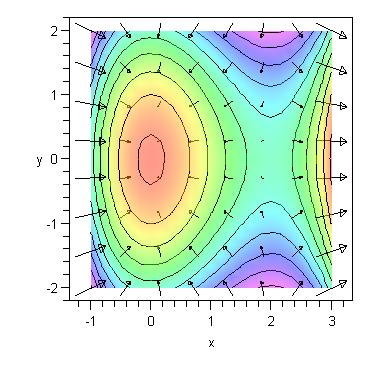
\includegraphics[width=\mywidth]{08-Optimization/support/levelcurve-1}
 
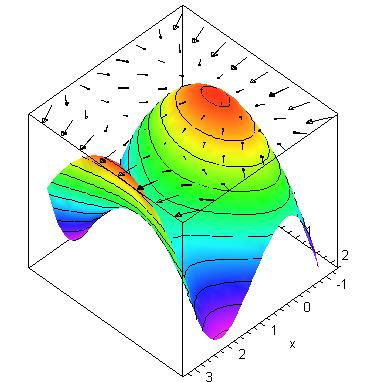
\includegraphics[width=\mywidth]{08-Optimization/support/levelcurve-2}&
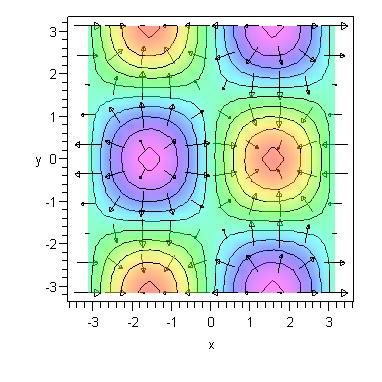
\includegraphics[width=\mywidth]{08-Optimization/support/levelcurve-3}&
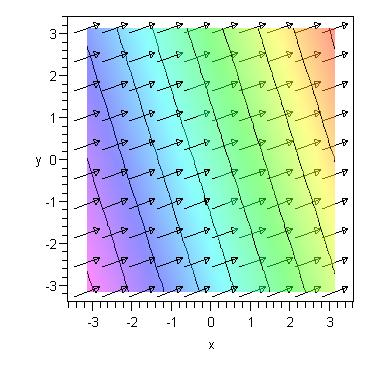
\includegraphics[width=\mywidth]{08-Optimization/support/levelcurve-4}&
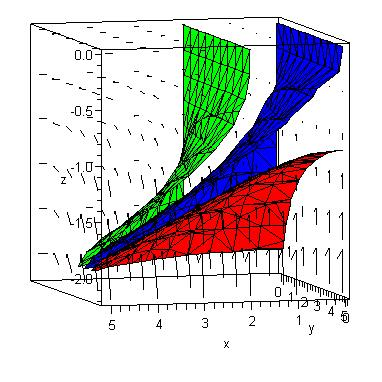
\includegraphics[width=\mywidth]{08-Optimization/support/levelsurface}\\
$f=x^3-3x^2-y^2+2$&
$f=\sin x\cos y$&
$f=3x+y$&
$f=x^2+yz^3$
\end{tabular}
\end{center}

\section{Directional derivatives}


For a function $z=f(x,y)$, the partial derivatives $f_x$ and $f_y$
give the slope of the function in the $x$ and $y$ directions,
respectively.  Furthermore, we know that the slope of the function is
zero in the directions that are orthogonal to the gradient at a point
from the previous sections.  Now we will calculate the slope of the
function in \emph{any} direction.

Let {$\vec u = \langle u_1,u_2\rangle$} be a unit vector
(representing any direction), and {$\vec p=(a,b)$} a point in the domain of
$f$. The directional derivative of $f$ in the direction of $\vec u$ at
the point $p=(a,b)$ is 
$$\ds D_{\vec u} f (\vec p) = \lim_{h\to
  0}\frac{f(\vec p + h\vec u) - f(\vec p)}{h}.$$ Geometrically, the
directional derivative is the slope of a tangent line to the surface
at $(a,b,f(a,b))$ which lies in a vertical plane containing the vector
$\langle u_1,u_2,0\rangle$ and the line $\vec q(t)=\langle a+u_1t,
b+u_2t\rangle$. The intersection of this vertical plane with the
surface is the space curve $\vec r(t) = \langle a+u_1t,b+u_2t,
f(a+u_1t,b+u_2t)\rangle=\langle a+u_1t, b+u_2t,f(\vec q(t))\rangle$,
which passes through the point $(a,b,f(a,b))$ at $t=0$.  The chain
rule gives the derivative of $\vec r$ at $t=0$ as $\vec r^\prime(0) =
\langle u_1,u_2,Df(\vec q(0))D\vec q(0)\rangle = \left<
  u_1,u_2,\begin{bmatrix}f_x(\vec p) & f_y(\vec
    p)\end{bmatrix}\begin{bmatrix}u_1\\u_2\end{bmatrix}\right> =
\langle u_1,u_2,\nabla f(\vec p)\cdot \vec u \rangle $. One unit
increase in the $\vec u$ direction gives a rise in the $z$ direction
of $\nabla f(a,b)\cdot \vec u$ units.  Hence we see that the
directional derivative is $$D_{\vec u} f (\vec p) = \nabla f(\vec
p)\cdot \vec u.$$ Since $\vec u$ is a unit vector, we can think of the
directional derivative in the direction $\vec u$ as the projection of
the gradient onto $\vec u$, i.e., $$D_{\vec u}f(\vec p) = \proj_{\vec
  u}\nabla f(\vec p).$$

Since $D_{\vec u} f (\vec p) = \nabla f(\vec p)\cdot \vec u = |\nabla
f(\vec p)||\vec u|\cos\theta$, where $\theta$ is the angle between
$\nabla f(\vec p)$ and $\vec u$, we see that the directional
derivative is greatest when $\cos\theta=1$, i.e., when $\theta =
0$. The direction of greatest increase is given by the gradient.  The
direction of greatest decrease is opposite the gradient, where
$\theta=\pi$.  The function does not increase or decrease (i.e., it
stays level) where $\theta=\pi/2,-\pi/2$.  In these directions are the
contour lines of the function.  In other words, the gradient is
orthogonal to the contour lines of the function.  This matches up with
what we saw previously.


Recall the differential notation $dy=f' dx$ from first-semester
calculus.  This can be extended to all dimensions as $d\vec y=D\vec f
d\vec x$, or $d(\text{outputs}) =Df d(\text{inputs})$. For a function
$z=f(x,y)$, we have
$dz=\begin{bmatrix}f_x&f_y\end{bmatrix}\begin{bmatrix}dx\\dy\end{bmatrix}$.
If $\vec u =\langle u_1,u_2\rangle$ is a unit vector, then a change in the inputs
$dx=u_1$ and $dy=u_2$ gives a change in the output $dz$ as the
directional derivative in the direction of $\vec u$. We again have
$D_{\vec u} f (\vec p) = D f(\vec p)\vec u = \nabla f(\vec p)\cdot \vec u$.
Interpretations about the gradient come immediately when you use the
differential notation $d(\text{outputs}) =Df d(\text{inputs})$.



\begin{example}
 \marginpartop{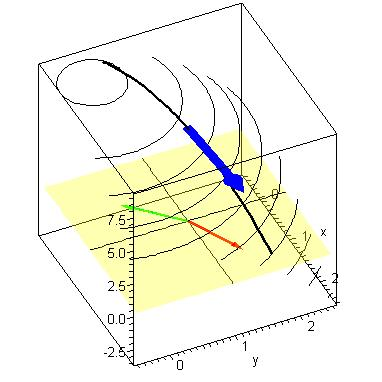
\includegraphics[width=\marginparwidth]{08-Optimization/support/dirder}}%
The function $f(x,y)=9-x^2-y^2$ has deriviative
$Df=\begin{bmatrix}-2x&-2y\end{bmatrix}$, i.e. $\nabla f = \langle-2x,-2y\rangle$ The
directional derivative in the $\vec u = \langle1,0\rangle$ direction at some point
point $(x,y)$ is $D_{\vec u}f(x,y)=\langle-2x,-2y\rangle\cdot\langle1,0\rangle=-2x$, or the
derivative in the $x$ direction.  The directional derivative in the
direction $\langle2,1\rangle$ (which as a unit vector is
$\frac{1}{\sqrt{5}}\langle2,1\rangle$) is
$D_{\langle2,1\rangle}f(x,y)=\langle-2x,-2y\rangle\cdot\frac{1}{\sqrt{5}}\langle2,1\rangle=\frac{1}{\sqrt{5}}(-4x-2y)$.
At the point $(1,1)$, we have $\nabla f(1,1) = \langle-2,-2\rangle$ and
$D_{\langle2,1\rangle}f(1,1)=\langle-2,-2\rangle\cdot \frac{1}{\sqrt 5}\langle2,1\rangle=-\frac{6}{\sqrt{5}}$.
The direction of greatest increase at $(1,1)$ is in the $\langle-2,-2\rangle$
direction. This is illustrated in the picture to the left. The $xy$
plane is shaded in the picture. The direction of the gradient points
back to the origin (it is a 2D vector).  The direction of $u$ points
away from the origin (hence the dot product is negative). Several
level curves of $f$ are drawn in 3D with their height included.  The
space curve shown is a curve in the surface. A tangent vector to that
curve is also drawn. The change in height of that tangent vector is
the directional derivative, as the change in the $xy$ direction is 1
unit.
\end{example}



\section{Tangent planes and Approximation}
Since the gradient is normal to level surfaces, the gradient $\nabla
f(x,y,z)$ of function $f(x,y,z)$ can be used to find the tangent plane
to level surfaces.  For example, the hyperboloid of one sheet
$1=x^2+y^2-z^2$ is the level surface $f=1$ of the function
$f=x^2+y^2-z^2$. The point $(1,-2,2)$ is on this hyperboloid, so the
gradient $\nabla f(x,y,z)=\langle2x,2y,-2z\rangle$ evaluated at $(1,-2,2)$ gives the
vector $\nabla f(1,-2,2)= \langle2,-4,-4\rangle$, which is a normal vector for the
tangent plane to the hyperboloid at $(1,-2,2)$.  An equation of the
tangent plane is thus $2(x-1)-4(y+2)-4(z-2)=0$. 

If a surface can be written in the form $z=f(x,y)$, then the function
$g(x,y,z) = z-f(x,y)$ has as its gradient $\nabla g = \langle-f_x,-f_y,1\rangle$.
Hence, a normal vector to the tangent plane of a surface $z=f(x,y)$ is
$\vec n = \langle-f_x,-f_y,1\rangle$, which we already discovered as $\vec n =
\langle1,0,f_x\rangle\times\langle0,1,f_y\rangle$.

The differential {$dy=f^\prime dx$} says a little change in {$y$} can be
approximated by multiplying the derivative by a little change in
{$x$}.  For a function $f\colon \mathbb{R}^n\to\mathbb{R}^m$, the
\textbf{differential} is $d\vec y = D\vec f d\vec x$, where $D\vec f$
is the derivative, {$d\vec y$} is an $m$ dimensional vector of changes
in the outputs, and {$d\vec x$} is an $n$ dimensional vector of
changes in the inputs. We estimate changes in our outputs by
multiplying the derivative by changes in our inputs.
For a function $z=f(x,y)$, this gives $dz=f_xdx+f_ydy$. If we write
our change in inputs as $\langle dx,dy\rangle = \vec u ds$ for a unit vector $\vec
u$ with magnitude $ds$, then a change in  $z$ is approximately $dz =
Df\vec u ds= D_{\vec u}f ds$, or the product of the directional
derivative and $ds$.

\note{Follow this order: think of the approximation as traveling a bit of distance along the directional vector (and do a problem as such).  Then think of it as $d\vec y=D\vec f d\vec x$, and work the same problem that way.}

The differential formula $d\vec y=D\vec f d\vec x$ can be used to
connect ideas about tangent lines, tangent planes, and approximation
in all dimensions.  The following table summarizes how to use this
notation in various settings.
\begin{center}
\begin{tabular}{|c|c|c|c|c|c|}
\hline
Function & $d\vec y$ & $Df$ & $d\vec x$ & $\vec x=\vec c$ & Tangent
space (line, plane, etc.)\\
 &  &  &  &  & $d\vec y = D\vec f(\vec c) d\vec x$\\
 &  &  &  &  & $\vec y - \vec f(\vec c) = D\vec f(\vec c) (\vec x-\vec
c)$\\\hline
$y=f(x)$ & $dy$ & $f^\prime$ & dx & $x=c$& $y - f(c) = f^\prime(c) ( x -
c)$\\\hline

$\vec r(t)=\langle x,y,z\rangle$ & $\begin{bmatrix}dx\\dy\\dz\end{bmatrix}$ &
$\begin{bmatrix}x^\prime(t)\\y^\prime(t)\\z^\prime(t)\end{bmatrix}$ & $dt$ & $t=c$& 
$\begin{bmatrix}x-x(c)\\y-y(c)\\z-z(c)\end{bmatrix} =
\begin{bmatrix}x^\prime(c)\\y^\prime(c)\\z^\prime(c)\end{bmatrix} ( t - c)$\\\hline

$z=f(x,y)$ & $dz$ & $\begin{bmatrix}f_x&f_y\end{bmatrix}$ &
$\begin{bmatrix}dx\\dy\end{bmatrix}$ & $(x,y)=(a,b)$ & $z-f(a,b) =
\begin{bmatrix}f_x(a,b)&f_y(a,b)\end{bmatrix}
\begin{bmatrix}x-a\\y-b\end{bmatrix}$\\\hline

$\vec r(u,v)=\langle x,y,z\rangle$ & $\begin{bmatrix}dx\\dy\\dz\end{bmatrix}$ 
& $\begin{bmatrix}x_u &x_v\\y_u&y_v\\z_u&z_v\end{bmatrix}$ 
& $\begin{bmatrix}du\\dv\end{bmatrix}$
& $(u,v)=(a,b)$& $
\begin{bmatrix}x-x(a,b)\\y-y(a,b)\\z-z(a,b)\end{bmatrix} =
\begin{bmatrix}x_u &x_v\\y_u&y_v\\z_u&z_v\end{bmatrix}
\begin{bmatrix}u-a\\v-b\end{bmatrix}$\\\hline

\end{tabular}
\end{center}
A change $d\vec y$ in output is the output variable $\vec y$ minus its
value $\vec f(\vec c)$ at the input $\vec c$. A change $d\vec x$ in
the input is the variable $\vec x$ minus its value at $\vec c$.
Tangent planes can be found in all dimensions using this notation.

\begin{example}
We can use differential notation to estimate changes in a function. If
the temperature at a point in the plane is given by
{$T(x,y)=x^2-xy-y^2$} degrees Fahrenheit, and a particle is at
{$(2,3)$}, estimate the change in temperature if the particle moves
about .1 units in the direction of {$\langle3,4\rangle$}. The gradient of $T$ is
$\nabla T = \langle2x-y,-x-2y\rangle$, which at $(2,3)$ is $\nabla T(2,3) = \langle1,-8\rangle$. The
change in inputs is $\langle dx,dy\rangle = .1\frac{\langle3,4\rangle}{|\langle3,4\rangle|} =
\frac{.1}{5}\langle3,4\rangle = \langle.06,.08\rangle$.  We calculate the change in
temperature (the output) as $dT = DT(2,3)
\begin{bmatrix}dx\\dy\end{bmatrix} = T_x dx+T_ydy = (1)(.06)+(-8)(.08)
= -.58$. So the temperature will decrease a little over half a degree.   
\end{example}

\begin{example}
A rectangle is rather wide and short.  When you measure the edges of
the rectangle to estimate the area, which edge must be measured more
precisely to not affect the area of the rectangle?  Area is
$A(h,w)=hw$, so $dA =
\begin{bmatrix}A_h&A_w\end{bmatrix}\begin{bmatrix}dh\\dw\end{bmatrix}
= \begin{bmatrix}w&h\end{bmatrix}\begin{bmatrix}dh\\dw\end{bmatrix} =
wdh+hdw$. Since $w$ is large, a small change $dh$ in the measurement
of the height will have a much larger affect on the change in area. 
Hence, you must be more precise when measuring the shorter height.
\end{example}

\begin{example}
The total resistance {$R$} in a circuit with two parallel resistors
with resistance {$R_1$} and {$R_2$} is given by the formula {$
\frac{1}{R} = \frac{1}{R_1}+\frac{1}{R_2} $}.  Solving for $R$ and
taking derivatives, one can show that {$ dR =
\begin{bmatrix}\frac{R^2}{R_1^2} & \frac{R^2}{R_2^2} \end{bmatrix}
\begin{bmatrix}dR_1\\dR_2\end{bmatrix}$}. If {$ R_1 $} changes from 10
to 9.9, and {$ R_2 $} changes from 20 to 20.2, would you expect a
positive or negative change in the total resistance {$R$}? We have
$dR_1 = -.1$ and $dR_2=.2$, and $\frac{1}{R} = \frac{3}{20},$ so
$R=20/3$ and $dR = \begin{bmatrix}\frac{(20/3)^2}{10^2} &
\frac{(20/3)^2}{20^2} \end{bmatrix}
\begin{bmatrix}-.1\\.2\end{bmatrix} = 
(2/3)^2(-.1) + (1/3)^2(.2) = -4/90+2/90=-2/90<0$ which is negative.
Manufactures of circuit boards have to account for variations in the
resistance of resistors.  Differentials allow them to estimate total
changes in resistance due to possible changes in each resistor. 
\end{example}

% \subsection{Local Linearization}
% The textbook discusses the ``Local linearization'' of a function as
% $L(x,y) = f(a,b) + f_x(a,b)(x-a)+f_y(a,b)(y-b)$, which is equivalent
% to $L(x,y)-f(a,b) = df$, or $L=f+dz$ (just add the function to the
% change in the function to get an approximate value for the function at
% $(x,y)$).  The error $dz = L(x,y)-f(a,b)$ in approximating $f$ is also
% called $E(x,y)$ in the book.  You can estimate how much error there is
% by the formula {$ |E|\leq\frac{1}{2}M(|dx|+|dy|)^2 $}, where $M$ is any
% upper bound for the values $|f_{xx}|,|f_{yy}|$, and $|f_{xy}|$. The
% value of this formula is that it tells you how far off the change $dz$
% could be from the real change $\Delta z = f(x+dx,y+dy)-f(x,y)$ in output.

\section{The Second Derivative Test}
If a function $y=f(x)$ has a relative extremum at $x=c$, then
$f^\prime(c)=0$ or the derivative is undefined. The places where the
derivative is either zero or undefined are called critical values of
the function. The first derivative test allows you to check the value
of the derivative on both sides of the critical value and then
interpret whether that point is a maximum or minimum using
increasing/decreasing arguments.  The second derivative test requires
you to compute the second derivative at $x=c$. If $f^{\prime\prime}(c)>0$ (the
function is concave upwards), then the function has a minimum at
$x=c$. If $f^{\prime\prime}(c)<0$ (the function is concave downwards), then the
function has a maximum at $x=c$. If $f^{\prime\prime}(c)=0$, then the second
derivative test fails.

The first derivative test breaks down in higher dimensions because
there are more than two ways to approach a point of the domain. All that
can be said is that at an extreme value, the gradient is zero (as the
tangent plane should be horizontal). In higher dimensions, there are
three classifications of critical points: maximum, minimum, saddle
point (a point where the tangent plane is horizontal, but in some
directions you increase and in other directions you decrease). The
second derivative test does not break down. To understand the second
derivative test, we need to learn about eigenvalues and eigenvectors
of a matrix.

If {$z=f(x,y)$}, then $Df(x,y) = \begin{bmatrix}f_x&f_y\end{bmatrix}$
is a vector field with two inputs and two outputs. Its derivative
{$D^2f (x,y)= \begin{bmatrix}f_{xx}&f_{xy}\\f_{yx}&f_{yy}\end{bmatrix}
  $} is a {$2\times 2$} square matrix called the Hessian of $f$. This
matrix is symmetric (i.e., $f_{xy}=f_{yx}$) if $f$ is twice
continuously differentiable.

An eigenvector is a vector (direction), such that multiplication by
the matrix is the same as multiplying the vector by a scalar (that
scalar is called an eigenvalue). Notationally this is written {$ A\vec
v=\lambda \vec v $}, where {$ \lambda $} is the eigenvalue and $\vec v$ is an
eigenvector. Eigenvalues can be found by subtracting {$\lambda$} from each
of the entries on the diagonal of a square matrix, and then asking for
which values of {$\lambda$} the determinant equals zero (solve {$ \det(A-\lambda I)
= 0 $}). In linear algebra, you will learn much more about
eigenvectors and eigenvalues. For example, the eigenvalues of the
matrix {$ \begin{bmatrix}2&1 \\1&2\end{bmatrix} $} are found as
follows. Write {$ \det \begin{bmatrix}2-\lambda&1 \\1&2-\lambda\end{bmatrix} =0$}.
Compute the determinant and set it equal to zero: {$(2-\lambda)(2-\lambda)-(1)(1) = 0$} or {$4-4\lambda + \lambda^2 -1 = 0$}. Hence
{$\lambda^2-4\lambda +3 = (\lambda-3)(\lambda -1) = 0$} or the eigenvalues are {$\lambda = 1,3$}. 

Another way to find eigenvalues follows from some linear algebra
theorems that we won't prove.  First, for a square matrix, the
determinant is the product of the eigenvalues.  Second, the sum of
diagonal elements (the \emph{trace} of the matrix) is the sum of the
eigenvalues.  This makes it easy to solve for the eigenvalues of a $2\times
2$ matrix.  For the example above, the determinant of $
\begin{bmatrix}
  2&1\\1&2
\end{bmatrix}$ is $4-1=3$ and the trace is $4$.  We need to find two
numbers such that the product is 3 and the sum is 4.  That is, $xy=3$
and $x+y=4$.  You may have already guessed that the values are $1$ and
$3$.  Therefore, $x=4-y$, so $(4-y)y=3$, so $y^2-4y-3=0$.  Solving
this for $y$ gives $y=1,3$.  Substituting and solving for $x$ then
gives us $x=3,1$, respectively.  In either case, we see that the
eigenvalues are $1$ and $3$.


%The notation {$D^2f$} for {$y=f(x)$} gives a {$1\times 1$} matrix
% $[f^{\prime\prime}(x)]$. The eigenvalue of this matrix is $f^{\prime\prime}(x)$. The
% second derivative test checks to see if that eigenvalue is positive or
% negative at a critical value.
%\begin{enumerate}
%	\item If the eigenvalue is positive at a critical point$x=c$,
% then the function is concave upwards and we have found a minimum.
%  \item If the eigenvalue is negative at a critical point$x=c$, then
% the function is concave downwards and we have found a maximum.
%\end{enumerate}

The eigenvalues of $D^2f$ give the ``directional'' second derivative
in the direction of a corresponding eigenvector. The largest
eigenvalue is the largest possible value of the second derivative in
any direction. The smallest eigenvalue is the smallest possible value
of the second derivative in any direction. The \textbf{second
derivative test} follows: If the eigenvalues are all positive at a
critical point, then in every direction the function is concave
upwards, which means that the function has a minimum at that critical
point.  If all the eigenvalues are negative, then in every direction
the function is concave downwards, and function has a maximum there. 
If there is a positive eigenvalue and a negative eigenvalue, the
function has a saddle point there.  If either the largest or smallest
eigenvalue is zero, then the second derivative test fails. 

%In higher dimensions, the second derivative test requires that we
% first locate all critical values $(a,b)$ where the gradient of {$f$}
% is the zero vector. Then find the eigenvalues of {$D^2f(a,b)$} (notice
% that you have to evaluate the derivative at the critical point). One
% of the following 4 options occurs.
%\begin{enumerate}
%	\item If all the eigenvalues are positive, then in every
% direction the function {$f$} is concave upwards, which means that you
% have found a minimum at $(a,b)$.
%	\item If all the eigenvalues are negative, then in every
% direction the function {$f$} is concave downwards, which means that
% you have found a maximum at $(a,b)$.
%	\item If some eigenvalues are positive and some are negative,
% then you have found a saddle point at $(a,b)$.
%	\item If either the largest eigenvalue or smallest eigenvalue
% is zero, then the second derivative test fails.
%\end{enumerate}

%
%For the function {$f(x,y)=x^2+4x+y^2-2y$}, the gradient is $Df =
% \begin{bmatrix}2x+4&2y-2 \end{bmatrix}$, which is zero at $x=-2,y=1$.
% The Hessian is $D^2f = \begin{bmatrix}2&0 \\0&2\end{bmatrix}$. The
% eigenvalues are found by solving $0=\det \begin{bmatrix}2-\lambda &0 \\0&2-\lambda
% \end{bmatrix} = (2-\lambda)^2$, so $\lambda =2$ is a double root.  Since all the
% eigenvalues are positive, the function is concave up in every
% direction at $(-2,1)$, which means that $f(-2,1)=-5$ is a minimum
% value of $f$. 


\begin{example} 
  For the function {$f(x,y)=x^2-6xy+y^2$}, the gradient is $Df =
  \begin{bmatrix}2x-6y&-6x+2y \end{bmatrix}$, which is zero only at
  $x=0,y=0$ (solve the system of equations $2x-6y=0,-6x+2y=0$). The
  Hessian is $D^2f = \begin{bmatrix}2&-6 \\-6&2\end{bmatrix}$. The
  eigenvalues are found by solving $0=\det \begin{bmatrix}2-\lambda
    &-6 \\-6&2-\lambda \end{bmatrix} = (2-\lambda)^2-36 =
  4-4\lambda+\lambda^2 -36 = (\lambda-8)(\lambda+4)$, so $\lambda =
  8,-4$ are the eigenvalues.  Since there is a positive eigenvalue and
  a negative eigenvalue, the function is concave upwards in one
  direction and concave downwards in another direction, so there is a
  saddle point at the origin.
\end{example}

\begin{example}
  For the function {$f(x,y)=x^3-3x+y^2-4y$}, the gradient is $Df =
  \begin{bmatrix}3x^2-3&2y-4 \end{bmatrix}$, which is zero at
  $x=1,y=2$ or $x=-1,y=2$. Hence there are two critical points. The
  Hessian is $D^2f = \begin{bmatrix}6x&0 \\0&2\end{bmatrix}$. Since
  there are two critical points, we have to find the eigenvalues of
  two matrices.  When $x=-1,y=2$, the eigenvalues of
  $\begin{bmatrix}-6&0 \\0&2\end{bmatrix}$ are $\lambda=-6,2$. Since
  one is positive and one is negative, there is a saddle point at
  $(-1,2)$. When $x=1,y=2$, the eigenvalues of $\begin{bmatrix}6&0
    \\0&2\end{bmatrix}$ are $\lambda=6,2$.  Since both are positive,
  there is a minimum at $(-1,2)$ (as in every direction the function
  is concave upwards).
\end{example}

\begin{example}
  We can use these ideas to find the dimensions of the rectangular
  prism of maximum volume that is located above the {$xy$} plane, and
  below the paraboloid {$z=9-x^2-y^2$}. We want to maximize the
  function $V(x,y) = (2x)(2y)(9-x^2-y^2)$.  The gradient is zero at
  $x=3/2,y=3/2$, and the Hessian at that critical point is
  $\begin{bmatrix}-54&-18 \\-18&-54\end{bmatrix}$. The eigenvalues are
  $\lambda = -36,-72$, which are both negative, which means we have
  found a maximum. I skipped a lot of details which you can check. The
  maximum volume is $f(3/2,3/2)=81/2$ and occurs at $(3/2,3/2)$. Since
  $x$ is only half the length, the dimensions are $3$ by $3$ by $9/2$.
\end{example}

If the domain of a function is restricted to a small region, then you
use the second derivative test to find the optimum solutions on the
interior of the domain.  You use the first derivative test on the
boundary of the domain to find the optimum solutions on the boundary.
If a function is continuous on a domain that is closed (includes its
boundary) and bounded, then there will always be a maximum and minimum
(this is called the extreme value theorem).


\section{Lagrange Multipliers}

To optimize a function {$f$}, subject to a constraint (such as a
height restriction, or a budget constraint for a business), we use a
technique called Lagrange Multipliers. Let {$f$} be the function you
want to optimize and {$g = 0$} be the constraint. Define $L=f-\lambda
g$ for some scalar lambda which will be determined. Find where all
partial derivatives of {$L$} are zero.  Under suitable conditions, the
optimum solutions will be a solution of $\nabla L=\vec 0$.  In other
words, the optimum solutions will be a solution of the equations
$\nabla f = \lambda \nabla g$ and $g==0$.

\begin{example}
  To find the dimensions of the rectangular prism of maximum volume
  that is located above the {$xy$} plane, and below the paraboloid
  {$z=9-x^2-y^2$}, we want to optimize the volume function
  $f(x,y,z)=4xyz$.  Our constraint is the height of $z$, which we
  rewrite as $g(x,y,z)=z-(9-x^2-y^2)=0$.  The Lagrangian is
  $L(x,y,z,\lambda)=4xyz - \lambda(z-9+x^2+y^2)$, and so the partials
  of $L$ are $L_x = 4yz-2\lambda x, L_y=4xz-2\lambda y,
  L_z=4xy-\lambda, L_\lambda = -(z-9+x^2+y^2)$. We now set each
  partial equal to zero and solve the system of equations.  We solve
  the first three equations for $\lambda$ to obtain $\lambda =
  \frac{4yz}{2x} = \frac{4xz}{2y}= \frac{4xy}{1}$.  The equation
  $\frac{4yz}{2x} = \frac{4xz}{2y}$ means $y^2=x^2$ or $x=y$ as the
  values for $x$ and $y$ must both be positive.  The equation
  $\frac{4xz}{2y}= \frac{4xy}{1}$ means $4z=8y^2$ or $z=2y^2$.  The we
  now substitute $x=y$ and $z=2y^2$ into the equation
  $L_\lambda=-g(x,y,z)=0=-(z-9+x^2+y^2)$ to obtain $2y^2-9+y^2+y^2=0$
  or $y^2=9/4$ so $y=3/2$.  Hence $x=3/2,z=9/2$ and the dimensions are
  $3$ by $3$ by $9/2$.
\end{example}

\begin{example}
  To find the point closest to the origin on the hyperbolic cylinder
  {$x^2-z^2=1$}, we want to optimize the distance
  $f=\sqrt{x^2+y^2+z^2}$ subject to the constraint
  $g=x^2-z^2-1=0$. However, the square root in the optimization
  function will result in rather messy derivatives, so instead we
  notice that distance is minimized at the same places where distance
  squared is minimized, so we can use $f=x^2+y^2+z^2$ instead.  The
  Lagrangian is $L=x^2+y^2+z^2-\lambda(x^2-z^2-1)$. The gradient is
  $\nabla L(x,y,z,\lambda) = \langle2x-2\lambda x, 2y, 2z+2\lambda x,
  -(x^2-z^2-1)\rangle$. We now solve for when the gradient is zero to
  obtain $2x-2\lambda x = 2x(1-\lambda)=0, 2y=0, 2z(1+\lambda)=0$ for
  the first three equations.  From the first equation we have $x=0$ or
  $\lambda=1$. However the constraint $x^2-z^2=1$ (which is
  $L_\lambda=0$) shows that $x\neq 0$, which means that $\lambda=1$.
  The second partial tells us that $y=0$, and the third partial shows
  us that $2z(2)=0$ or $z=0$.  Since $z=0$, we have using our
  constraint again that $x=\pm 1$. So there are two solutions
  $(-1,0,0)$ and $(1,0,0)$.
\end{example}



\subsection{Why Lagrange Multipliers works - linear dependence}
If the domains of {$f$} and the constraint $g$ are 2 dimensional, then
{$g=0$} represents a level curve of the function {$g$}. At a maximum
of {$f$} where {$g=0$}, the level curve of {$f$} which passes through
the location of the maximum will have a tangent line that is parallel
to the level curve of {$g$}.  Hence, the gradients of {$f$} and {$g$}
should be parallel, as they are normal to level curves (and since they
are normal to the same tangent line, they should be parallel). Hence
the gradient of {$f$} is a scalar multiple of the gradient of {$g$}. 
Call that scalar {$\lambda$}.  Then {$\nabla f=\lambda\nabla g$}. Hence, at a maximum or
minimum we will have {$0=\nabla f-\lambda\nabla g$}.  This is equivalent to solving 
{$\nabla L =\vec 0$}.


If the domains of {$f$} and the constraint are 3 dimensional, then
{$g=0$} represents a level surface of the function {$g$}. At a maximum
of {$f$} where {$g=0$}, the level surface of {$f$} which passes
through the location of the maximum will have a tangent plane that is
tangent to the level surface {$g=0$}.  Hence, the gradients of {$f$}
and {$g$} should be parallel as they are both normal vectors to the
same tangent plane.  So the gradient of {$f$} is a scalar multiple of
the gradient of {$g$}.  This line of reasoning extends to all
dimensions.


If you have multiple constraints, then let the Lagrangian be
{$L=f-\lambda_1g_1-\lambda_2g_2-\cdots$}. Under suitable conditions,
it can be shown that optimum solutions will satisfy the equation
{$\nabla L = 0$}. Just keep subtracting a new variable times the next
constraint for each new constraint. This works precisely because at an
optimal solution, it can be shown that the gradient of $f$ is a linear
combination of the gradients of the constraints, i.e. $\nabla f =
\lambda_1g_1+\cdots +\nabla_ng_n$. You will learn more about this
topic when you study linear algebra.

\section{Taylor Series}
Recall that a Taylor series centered at $x=a$ for a function $f(x)$ is
$\sum_{n=0}^{\infty}\frac{f^{(n)}(a)}{n!}(x-a)^n$.  This formula holds as well
for arbitrary functions if you replace $f^{(n)}(a)$ with the linear
transformation $D^n\vec f(\vec a)$ and write $\sum_{n=0}^{\infty}\frac{D^n\vec
  f(\vec a)}{n!}(\vec x-\vec a)^n$. However, interpreting this formula
requires knowledge about linear transformations, and becomes rather
messy to write in matrix notation. Quadratic forms appear as the
degree two term of the Taylor series.  You can use the Taylor series
to prove the second derivative test.  Further information can be found
by consulting the free textbook written by Kenneth Kuttler at BYU
Provo (though be warned that it is written for an advanced student).
For this book, see
\url{http://www.math.byu.edu/~klkuttle/calcbookB.pdf}.






%%% Local Variables: 
%%% mode: latex
%%% TeX-master: "../multivariable-calculus"
%%% End: 






\newgeometry{left=1in,right=1in,top=1in,bottom=1in}
\newpage

\section{Preparation}

\subsection{Lesson Plans}

This chapter covers the following ideas. When you create your lesson plan, it should contain examples which illustrate these key ideas. Before you take the quiz on this unit, meet with another student out of class and teach each other from the examples on your lesson plan. 

% A list of objectives for the chapter
%\begin{enumerate}
%\item ...
%\end{enumerate}

\begin{enumerate}
\item Explain the properties of the gradient, its relation to level
  curves and level surfaces, and how it can be used to find
  directional derivatives.  
\item Find equations of tangent planes using the gradient and level
  surfaces. Use the derivative (tangent planes) to approximate
  functions, and use this in real world application problems.
\item Explain the second derivative test in terms of eigenvalues.
  Illustrate how eigenvalues and eigenvectors are used to optimize
  functions of several variables.
\item Use Lagrange multipliers to optimize a function subject to
  constraints.  Explain why Lagrange multipliers works by considering
  the gradients of the function and the constraint at a maximum.
\end{enumerate}


%%% Local Variables: 
%%% mode: latex
%%% TeX-master: "../multivariable-calculus"
%%% End: 
%$


%\subsection{Preparation Problems}

%Here are the preparation problems for this unit.

\subsection{Homework}

In the following list, the ``basic practice'' problems should be quick
problems to help you master the ideas.  The ``good problems'' will
require a little more work.  The theory and application problems are
ones that will challenge you more; make sure you do the problems from
this area to fully master the material.  

\begin{center}
  \begin{tabular}{lcp{1.3in}p{1.3in}p{1.3in}}\toprule
    Topic & Section & Basic Practice & Good problems & Theory/Application \\\midrule
    Directional Derivative & 13.6 & 1--30, 55--62 & 31--50 & 51--54, 63--81\\
    Tangent planes & 13.7 & 1--18& 19--34, 41--46, 53--56 & 35--36, 47--48, 60--62\\
    Differentials & 13.4 & 1--20 & & 25--40\\
    Extrema & 13.8 & 7--15, 21--28 & 37--42, 45--50 & 17--20\\
    Applications & 13.9 & 5--8 & & 8--21\\
    Lagrange Multipliers & 13.10 & 1--12 & 13--22 & 31--44
  \end{tabular}
\end{center}


%%% Local Variables: 
%%% mode: latex
%%% TeX-master: "../multivariable-calculus"
%%% End: 


%%% Local Variables: 
%%% mode: latex
%%% TeX-master: "../multivariable-calculus"
%%% End: 

\restoregeometry


\chapter{Double Integrals}

This chapter covers the following ideas. 

% A list of objectives for the chapter
%\begin{enumerate}
%\item ...
%\end{enumerate}

\begin{enumerate}
\item Explain how to setup and compute a double integrals, as well as
how to interchange the bounds of integration. Use these ideas to find
area and volume.
\item For planar regions, find area, mass, centroids, center of mass,
moments of interia, and radii of gyration.
\item Explain how to change coordinate systems in integration, in
particular to a polar coordinates. Explain what the Jacobian of a
transformation is and how to use it.
\item Explain how to use Green's theorem to compute flow along and
flux across a curve.
\end{enumerate}

%%% Local Variables: 
%%% mode: latex
%%% TeX-master: "../multivariable-calculus"
%%% End: 
%$

\section{Double Integrals}

The integral $\int_a^b fdx$ represents the area of the region in the $xy$
plane above the interval $[a,b]$ along the $x$ axis under the curve
$f(x)$.  We will define a double integral $\iint_RfdA$ in such a
manner to obtain for positive $f(x,y)$ the volume of the solid region
in space above a region $R$ in the $xy$ plane under the surface
$z=f(x,y)$. To start with, we will assume that the region $R$ is a
rectangle $a\leq x\leq b$, $c\leq y\leq d$. Slice the rectangle up into many tiny
rectangles of dimensions $\Delta x_i,\Delta y_j$, making a grid for your region
$R$.  The area of each little subrectangle in the grid is $\Delta A_{ij} =
\Delta x_i\Delta y_j$.  If the grid is made so that $\Delta x_i$ and $\Delta y_j$ are both
really small, then the height of the surface $z=f(x,y)$ above a subrectangle is approximately constant, and can be approximated by the
value of $f$ at some point $f(x_i,y_j)$ in that subrectangle. This
gives an approximation for a small piece of volume as $\Delta V_{ij}\approx
f(x_i,y_j)\Delta A_{ij} = f(x_i,y_j)\Delta x_i\Delta y_j$.  Add up the small pieces
of volume to get total volume as $V\approx \sum_{i=1}^n\sum_{j=1}^m f(x_i,y_j)\Delta
x_i\Delta y_j$.  The double limit $V\approx
\lim_{n\to\infty}\lim_{m\to\infty}\sum_{i=1}^n\sum_{j=1}^m f(x_i,y_j)\Delta x_i\Delta y_j$, if it
exists, is called the double integral of $f$ over $R$, and we write
$\iint_R fdA$. This limit will always exist if the function is
continuous and bounded on $R$.

If a double integral over a rectangle $R$ exists, then it can be
computed using the formulas $\iint_R fdA = \int_a^b \left(\int_c^d f
dy\right)dx = \int_c^d \left(\int_a^b f dx\right)dy$. These last two
integrals are called iterated integrals.  First integrate the inside
integral with respect to the variable inside, then integrate the
result with respect to the outside variable.  

\begin{example}
  For example the integral 
  \begin{align*}
    \int_0^2 \left(\int_1^4 2x+4xy dy\right)dx
  &=\int_0^2 \left( \big[2xy+2xy^2 \big]_{y=1}^{y=4}\right)dx \\
  &=\int_0^2 36x dx =  \big[18x^2\big]_{x=0}^{x=2} \\
  &= 72    
  \end{align*}
gives the same answer as the integral 

\begin{align*}
  \int_1^4\left(\int_0^2 2x+4xy dx\right)dy &= \int_1^4\left(\big[x^2+2x^2y
    \big]_{x=0}^{x=2}\right)dy \\
  &= \int_1^4 4+8ydy = \big[4y+4y^2 \big]_{y=1}^{y=4} \\
  &=
  16+64 - (4 + 4) = 72.  
\end{align*}
\end{example}

The reason a double integral can be computed using either iterated
integral has to do with looking at cross sections.  Rather than
slicing $R$ into a grid using both $\Delta x$ and $\Delta y$, just pick one
direction in which to make slices.  For example, if we cut the region
$R$ along lines parallel to the $y$ axis, then each slice has a width
$\Delta x_i$, and we pick a point $x_i$ in each interval on the $x$ axis.
The area of the cross section of the plane $x=x_i$ under $z=f(x_i,y)$
above the $xy$ plane is given by the integral $A=\int_c^d f(x_i,y)dy$.
Multiply this area $\int_c^d f(x_i,y)dy$ by $\Delta x_i$ for each $i$ to
obtain an approximation for the volume above the $i$th slice of $R$,
i.e. $\Delta V_i\approx \int_c^d f(x_i,y)dy\Delta x_i$. Total volume is found by adding
up the little bits of volume and taking a limit as $\Delta x_i\to 0$. This
gives the volume as 
$V=\int_a^b \left(\int_c^d f dy\right)dx$.  Since the parenthesis take up
extra space, we write simply $\iint_R fdA = \int_a^b \int_c^d f \,dydx = \int_c^d
\int_a^b f \,dxdy$.

If the region $R$ is not a rectangle, but is bounded, and the function
$f$ is bounded for all $(x,y)$ in the region $R$, then we
(theoretically) define the
double integral by placing the region $R$ inside a rectangle which
contains $R$ and defining $f(x,y)=0$ for all $(x,y)$ not in $R$.  To
actually compute the double integral, we pick bounds for the integral which
describe our region.  The outer bounds of the integral must be two
constants. The inner bounds can be functions which involve variables
of the outer bounds.  The outer bounds represent two horizontal or
vertical lines.  The inner bounds represent two functions whose input
is the outer bound variable. 

\begin{example}
\marginpartop{
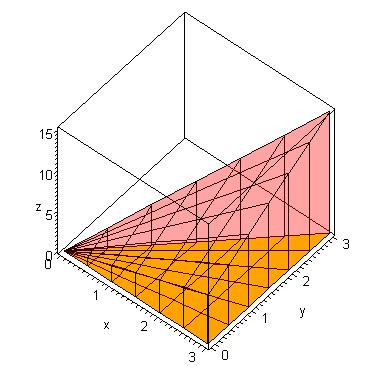
\includegraphics[width=\marginparwidth]{09-DoubleIntegrals/support/double-1}
}%
The volume of the region under the plane $z=2x+3y$ above the region
$R$ which is bounded by the lines $y=x,y=0,x=3$ can be found using a
double integral.  If we choose $y$ as the outer variable, and $x$ as
the inner variable, then we have to pick two constants which trap all
the $y$ values, and then pick two functions of $y$ which trap all the
$x$ values.  The constants are $0\leq y\leq 3$, and the functions are $y\leq x\leq
3$.  The corresponding double integral is $\int_0^3\int_y^3 2x+3y \,dxdy$.
Alternatively, if we choose $x$ as the outer variable and $y$ as the
inner variable, then $x$ is between the constants $0$ and $3$ ($0\leq x\leq
3$) and $y$ is between the functions $y=0$ and $y=x$ ($0\leq y\leq x$).  The
corresponding integral is $\int_0^3\int_0^x 2x+3y \,dydx$. Notice that the
integrand $2x+3y$, the $z$-value being summed, is the same in both
iterated integrals.  The region only affects the bounds of the
integrals and the order of the integration.
\end{example}

If $f=1$, then $\iint_R 1dA$ is the area of the region $R$.  Hence
area (a 2 dimensional quantity) is computed by adding up little bits
of area $dA$.  For the region $a\leq x\leq b$, $0\leq y\leq f(x)$, we have
$\iint_R 1 dA = \int_a^b\int_0^{f(x)}dydx = \int_a^b y\big|_0^{f(x)}dx = \int_a^b
f(x) dx$, which  is the formula found in first semester calculus.


\subsection{Switching the Order of Integration}
Sometimes it is valuable to switch the bounds of integration by
reordering the variables.  This is done by describing the region $R$
(often by constructing a graph), and then changing the way you
describe the region.  

\begin{example}
To compute the integral $\int_0^1\int_y^1
e^{x^2}\,dxdy$, we could first try to integrate the inside integral but
we would fail (as $\int e^{x^2}dx$ does not have an anti-derivative which
is an elementary function). So instead, we write the bounds as
inequalities $0\leq y\leq 1, y\leq x\leq 1$ and realize that the region describe
by these inequalities is the triangle in the first quadrant under the
line $y=x$ for $0\leq x\leq 1$.  Hence we can describe the region also as
$0\leq x\leq 1, 0\leq y\leq x$ which gives the integral $\int_0^1\int_0^x e^{x^2}\,dydx$.
The inner integral is now $\int_0^x e^{x^2}dy = ye^{x^2}\big|_0^x =
xe^{x^2}$.  Hence we have $\int_0^1\int_0^x e^{x^2}\,dydx = \int_0^1 xe^{x^2}dx$,
which is solved by letting $u=x^2$, $du=2xdx$, $dx=\frac{du}{2x}$,
$u(0)=0$, and $u(1)=1$, so $\int_0^1 xe^{x^2}dx = \int_{u=0}^{u=1} x
e^{u}\frac{du}{2x} =  \frac{1}{2}\int_{u=0}^{u=1} e^{u}du =
\frac{1}{2}e^u\big|_0^1 = \frac{1}{2}(e^1-e^0) = \frac{1}{2}(e-1)$.
\end{example}

\begin{example}
The region $R$ inside a circle of radius 3 above the $x$ axis can be
described as either $-3\leq x\leq 3$ and $0\leq y\leq \sqrt{9-x^2}$ or as $0\leq y\leq 3$ and
$-\sqrt{9-y^2}\leq x\leq \sqrt{9-x^2}$.  Hence the integral $\iint_R  1 dA$
can calculated as either $\int_{-3}^{3}\int_{0}^{\sqrt{9-x^2}}dydx$ or
$\int_{0}^{3}\int_{-\sqrt{9-y^2}}^{\sqrt{9-y^2}}\,dxdy$.  Both integrals give
the answer $9\pi/2$, which is the area of this region.  
\end{example}

\begin{example}\label{ex:double-integral}
The integral $\int_0^2\int_{x^2}^{2x}\,dydx$ gives the area of the region
between the curves $y=2x$ and $y=x^2$ and can also be written as
$\int_0^4\int_{y/2}^{\sqrt{y}}\,dxdy$.
\marginpar{
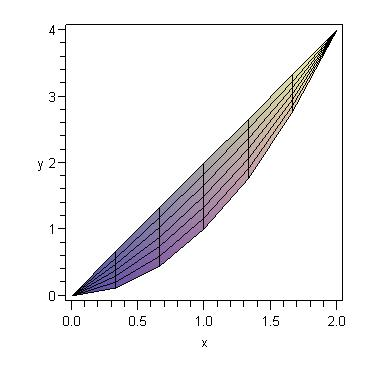
\includegraphics[width=\marginparwidth]{09-DoubleIntegrals/support/double-2}
\centering Example \ref{ex:double-integral}: $\int_0^2\int_{x^2}^{2x}dydx=\int_0^4\int_{y/2}^{\sqrt{y}}\,dxdy$
}%
\end{example}



\section{Changing Coordinate Systems: Generalized $u$-substitution}

To solve the definite integral $\int_0^3 e^{2x}dx$, we make a
substitution $u=2x$ or $x=u/2$, and then notice that $dx =
\frac{1}{2}du$.  Under this substitution, the interval $[0,3]$
transforms to the interval $[0,6]$ and the integral becomes $ \int_0^3
e^{2x}dx = \int_0^6 e^u\frac{1}{2}du$. Notationally, we can write this as
$\int_{C_x} f(x)dx = \int_{C_u} f(x(u))\frac{dx}{du}du$, where $C_x$ and
$C_u$ are the integration bounds in terms of $x$ and $u$ respectively,
and $x(u)=u/2$, so $\frac{dx}{du} = \frac{1}{2}$. Similarly, the
substitution $x=\tan \theta$ gives $\frac{dx}{d\theta}=\sec^2\theta$ and allows us to
compute $\int_0^1\frac{1}{1+x^2}dx =
\int_{0}^{\pi/4}\frac{1}{1+\tan^2\theta}\sec^2\theta d\theta = \int_0^{\pi/4}d\theta = \pi/4$, since
$\tan 0=0$ and $\tan (\pi/4) =1$.

To generalize this to higher dimensions we have to (1) change the
bounds of integration, and (2) replace $\frac{dx}{du}$ with the
generalized version in high dimensions.
To change the bounds in a new coordinate system requires that we
describe the exact same region using different coordinates.  We will
illustrate this with examples.  The term $\frac{dx}{du}$ in higher
dimensions is called the Jacobian of the transformation, and is the
absolute value of the determinant of the derivative of the change of
coordinates. 

\subsection{Polar Coordinates}
Polar coordinates are defined by $x=r\cos\theta, y=r\sin\theta$, which we can
represent using function notation as $T(r,\theta)=\langle r\cos\theta,
r\sin\theta\rangle$. Recall that the derivative of this transformation is 
$DT(r,\theta)= 
\begin{bmatrix}
\cos\theta&-r\sin\theta\\
\sin\theta&r\cos\theta
\end{bmatrix}$. 
The derivative measures small changes in $x,y$ based on small changes
in $r,\theta$.  Determinants calculate area (up to a plus or minus sign).
The determinant of the derivative measures the change in area which
occurs when you change from one coordinate system to another.  To get
a positive value for area, we take the absolute value of the
determinant of the derivative and write $\frac{\partial(x,y)}{\partial(r,\theta)} =
|\det(DT(r,\theta))| = |r\cos^2\theta+r\sin^2\theta| = |r|$. This quantity is called
the Jacobian of the polar transformation from $x,y$ coordinates to $r,\theta$
coordinates.  As long as $r>0$, we can drop the absolute value and we
have that the Jacobian is $\frac{\partial(x,y)}{\partial(r,\theta)}=r$.  So if we wish to
change from $x,y$ to $r,\theta$ coordinates, we use the formula
$\iint_{R_{xy}} f(x,y)\,dxdy = \iint_{R_{r\theta}}
f(T(r,\theta))\frac{\partial(x,y)}{\partial(r,\theta)}drd\theta =  \iint_{R_{r\theta}} f(T(r,\theta))rdrd\theta $.
In differential form, we can abbreviate this as $dA=dxdy = rdrd\theta$. In
other words, after you change all the $x$ and $y$ terms to $r$ and
$\theta$, you have to multiply the entire expression by $r$.

\begin{example}
The region inside a circle of radius $a$ in the plane is easily
described in polar coordinates as $0\leq r\leq a$ and $0\leq \theta\leq 2\pi$. As a
rectangular integral, we can find the area of a circle by writing
$\int_{-a}^a\int_{-\sqrt{a^2-x^2}}^{\sqrt{a^2-x^2}}1\,dydx$, which is a rather
difficult integral to compute. However if we change to polar
coordinates, then we compute $\int_0^a\int_0^{2\pi}rd\theta dr$ or
$$\int_0^{2\pi}\int_0^ardrd\theta  = \int_0^{2\pi}r^2/2\big|_0^ad\theta  = 2\pi a^2/2 = \pi a^2 $$
rather easily. When regions of integration involve circles or curves
that are easily described in polar coordinates, often a change from
rectangular to polar coordinates is extremely useful. 
\end{example}

\begin{example}\label{ex:polar-integral}
The volume of the region in space in the first octant which is below
the paraboloid $z=9-x^2-y^2$, above the $xy$-plane, and satisfying $x\geq
y$, can be found using the iterated double integral $$\iint_R 1 dA =
\int_{0}^{3/\sqrt{2}}\int_{x}^{\sqrt{9-x^2}}9-x^2-y^2\,dydx.$$
 The region $R$
in the $xy$ plane is described in polar coordinates more simply as $0\leq
\theta\leq \pi/4$ and $0\leq r\leq 3$. Changing to polar coordinates we have $z=9-(x^2+y^2)
= 9-r^2$ and then we compute the volume as $V=\int_0^{\pi/4}\int_0^3
(9-r^2)\,rdrd\theta$, which is a much easier integral to compute.
\marginpar{
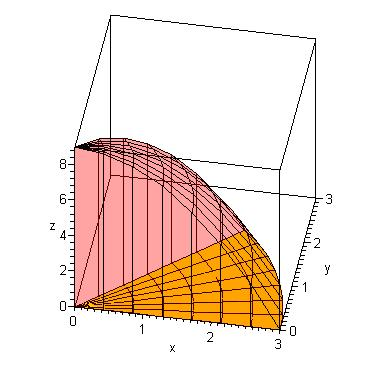
\includegraphics[width=\marginparwidth]{09-DoubleIntegrals/support/polar-1}
\centering Example \ref{ex:polar-integral}
}%
\end{example}

\subsection{General Change of coordinates}

In general, the Jacobian of a transformation $T$ is the absolute value
of the determinant of the derivative of the transformation, often
written $\frac{\partial(x,y)}{\partial(u,v)}$.  Polar coordinates is one of many
standard coordinate systems which people use. Some problems are simple
if you make the right substitution and very difficult if you don't. 
One advantage of working in higher dimensions is that you have the
ability to be creative and find the right change of coordinates to
solve a problem. Here are a few examples.

\begin{example}
To find the area inside of an ellipse
$\frac{x^2}{a^2}+\frac{y^2}{b^2}=1$, use the change of coordinates
$x=au,y=bv$.  The equation of the ellipse becomes $u^2+v^2=1$ in the
$uv$ coordinate system.  The Jacobian of this transformation is
$\left|\det \begin{bmatrix} a&0\\0&b\end{bmatrix}\right|=ab$, so we
have $A = \iint_R dxdy = \iint_{R_{uv}}abdudv = ab\iint_{R_{uv}}dudv$. 
Rather than actually compute the integral, recall that 
$\iint_{R_{uv}}dudv$ is the area of the region in the $uv$ plane,
which is the area inside a circle of radius 1, or $\pi$. Hence the area
of an ellipse is $ab\pi$. If you want a difficult challenge, try
computing this integral without this change of coordinates. 
\end{example}

\begin{example}
\marginpartop{
\aligntop{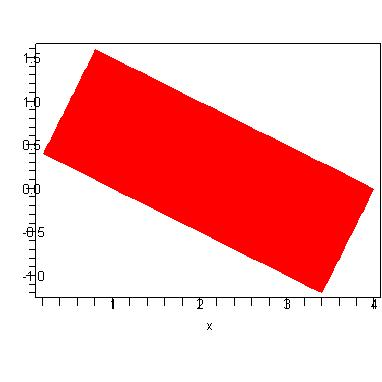
\includegraphics[width=\marginparwidth]{09-DoubleIntegrals/support/general-1}}
}%
If $R$ is the region in the plane bounded by the curves $x+2y=1$,
$x+2y=4$, $2x-y=0$, and $2x-y=8$, and we need to compute the integral
$\iint_R x\,dxdy$, then creating bounds for the integral is a rather
ugly mess.  Instead, we perform the change of coordinates $u=x+2y$ and
$v=2x-y$ (notice that for the first time we have $u$ and $v$ solved in
terms of $x$ and $y$). This change of coordinates transforms us to a
box $[1,4]\times [0,8]$ in the $uv$-plane.  To find the Jacobian of this
transformation, we need to first solve for $x$ and $y$ in terms of $u$
and $v$.  To eliminate $y$, we add $u+2v$ and get $5x$. Similarly,
eliminating $x$ gives $2u-v=5y$, so $x=\frac{u+2v}{5}$ and
$y=\frac{2u-v}{5}$.  The Jacobian of this transformation is
$$\left|\det \begin{bmatrix}
    1/5&2/5\\2/5&-1/5\end{bmatrix}\right|=\left|-1/25-4/25\right|=\left|-1/5\right|=1/5$$
(don't forget the absolute value).  Hence we have $$\iint_{R_{xy}}x\,dxdy
= \int_1^4\int_0^8\frac{u+2v}{5}\left(\frac{1}{5}\right)\,dvdu,$$ which is now
a fairly simple integral to compute.  The right change of coordinates
can simplify a problem.
\end{example}

In the previous problem, to find the Jacobian $\frac{\partial(x,y)}{\partial(u,v)}$,
we first solved for $x$ and $y$ in terms of $u$ and $v$. The ``Inverse
Function Theorem'' implies that $\frac{\partial(x,y)}{\partial(u,v)} =
1/\left(\frac{\partial(u,v)}{\partial(x,y)}\right)$. In other words, we could have
found the derivative of the transformation $T(x,y) = \langle u=x+2y,
v=2x-y\rangle$ as $\begin{bmatrix} 1&2\\2&-1\end{bmatrix}$, and then
after noticing that the absolute value of the determinant is $|-5|$,
we would invert this to obtain $\frac{\partial(x,y)}{\partial(u,v)} = \frac{1}{5}$.  So
you can either solve for $x$ and $y$ first, and then take the
determinant, or you can take the determinant and then invert the
result.  You get the same answer either way.


\section{Physical Applications}
Integrals are used in a wide variety of applications.  You should
notice that in most of the applications below, a formula which works
for double integrals is the same as the integral which we used for
line integrals.  The differentials $dx,ds,dA$ remind us which
dimension we are working in.  For lack of a better notation,  I will
use $d\square$ to represent any of these differentials when you are
free to pick the needed differential. The material which follows is
very similar to the work we did in the line integrals section. I start
by giving a summary of the differential formulas, and then we will use
them to find physical quantities.
\begin{itemize}
\item Area: $dA = fdx,fds, dxdy, rdrd\theta, \frac{\partial(x,y)}{\partial(u,v)}dudv$, 
\item Volume: $dV = fdA$, 
\item Average Value: $(\bar f)\square = \int fd\square$, 
\item Mass: $dm = \delta d\square , \delta dx, \delta ds, \delta dA$
\item Center of Mass: $(\bar x,\bar y,\bar z)m = \int\langle x,y,z\rangle
dm$, where $\int \bar x dm = \int x dm$ is a first moment of mass
\item Moment of Inertia: $I = \int r^2 dm$ is a moment of inertia, and $\int
R^2 dm = \int r^2 dm$ gives $R^2 m =I$ or $R=\sqrt{I/m}$
\end{itemize}
I strongly suggest that as you do each problem, start from a formula
in differential notation, and then modify it so that you have the
right number of integrals.  If you do this, you will learn how to do
calculus in all dimensions with ease. 

\begin{example}
Consider the region {$R = \{(x,y)\mid 0\leq x\leq 3, 0\leq y\leq x\} $} in the plane
with density function {$\delta(x,y) = x^2+y^2+1$}.  
Area is $A=\int_{0}^{3} \int_{0}^{x} dy dx$. Mass is $m=\iint_R dm=\int_{0}^{3}
\int_{0}^{x} (x^2+y^2+1)dy dx$. We can also compute
\begin{align*}
\bar y &= \frac{\int y dm}{\int dm}= \frac{\iint_R y \delta dA}{\iint_R \delta dA} =
\frac{\int_{0}^{3} \int_{0}^{x} y(x^2+y^2+1)dy dx}{\int_{0}^{3} \int_{0}^{x}
x^2+y^2+1dy dx}\\
R_x &= \sqrt{\frac{\int r^2 dm}{\int dm}} =\sqrt{\frac{\int y^2 dm}{\int dm}} =
\sqrt{\frac{\int_{0}^{3} \int_{0}^{x} y^2(x^2+y^2+1)dy dx}{\int_{0}^{3}
\int_{0}^{x} x^2+y^2+1dy dx}}
\end{align*}
\end{example}

\begin{example}
The temperature of a metal object covering the region {$R = \{(x,y)\mid 0\leq
x\leq 3, 0\leq y\leq x\} $} in the plane is given by {$f(x,y) = x^2+y^2+1$}. 
The area of the region $R$ is $A=\iint_R dA = \int_{0}^{3} \int_{0}^{x} dy
dx$ and the average temperature is $AV=\frac{1}{A}
\displaystyle\int_{0}^{3} \int_{0}^{x} x^2+y^2+1 dy dx$. 
\end{example}

\begin{example}
Consider a metal plate occupying the region in the plane bounded by
the curves {$x=y^2$} and {$y=x$}, with density function {$\delta(x,y) =
xy$}.  The mass of the plate is $m=\iint_R \delta dA = \int_0^1\int_{y^2}^{y}
(xy)\,dxdy$.
\end{example}
\begin{example}
The mass of the region in the plane bounded by the curves {$ x=2y $}
and {$ x=y^2 $}, with density {$ x^2+y^2 $}, is
$m=\int_0^2\int_{y^2}^{2y}(x^2+y^2) \,dxdy$. The center of mass is $\bar x =
\frac{1}{m}\int_0^2\int_{y^2}^{2y} x (x^2+y^2) \,dxdy$ and $\bar y =
\frac{1}{m}\int_0^2\int_{y^2}^{2y} y (x^2+y^2) \,dxdy$.
\end{example}

The centroids of many regions are geometrically obvious (such as the
center of a circle, square, or rectangle).   If a centroid is known,
then you can use this knowledge to simplify many integrals.  For
example, we can compute $\displaystyle \int_0^4\int_0^6 3x+5y \,dydx =
3\int_0^4\int_0^6 x \,dydx + 5\int_0^4\int_0^6 y \,dydx= 3\bar x A +5\bar y A = 3\cdot 2\cdot
24 + 5\cdot 3\cdot 24$, since the centroid of the rectangle $R=[0,4]\times[0,6]$ is
$(2,3)$ with area $24$.   





\section{Green's Theorem}





\subsection{Circulation Density }
Let $C$ be a simple closed curve parametrized so that it is traced
counter-clockwise (i.e., we say it is ``oriented counterclockwise'').
Recall that circulation of $\vec F$ along $C$ is
$\oint_C \vec F \cdot d\vec r$.  We now define circulation density for a vector
field $\vec F(x,y)=\langle M,N\rangle$ in the plane. At the point
$(x,y)$ in the plane, create a circle $C_a$ of radius $a$ centered at
$(x,y)$, where the area inside of $C_a$ is given by $A_a$. The
quotient $\frac{1}{A_a}\oint_{C_a} \vec F \cdot d\vec r$ is circulation per
area.  The limit $\lim_{a\to 0} \frac{1}{A_a}\oint_{C_a} \vec F \cdot d\vec r$ is
called the circulation density of $\vec F$ at $(x,y)$.  It can be
shown that $\lim_{a\to 0} \frac{1}{A_a}\oint_{C_a} \vec F \cdot d\vec r =
N_x-M_y$, and that $C_a$ can be replaced with a square of side lengths
$a$ centered at $(x,y)$ with interior area $A_a$ or any collection of
curves $C_a$ which ``shrink nicely'' to $(x,y)$. Regardless, $N_x-M_y$ is
circulation per unit area.

\begin{example}
For the vector field $\vec F = \langle-y,x\rangle$, the
circulation along a circle of radius $a$ is $2\pi a^2$.  Division by the
area $\pi a^2$ and taking a  limit gives $\lim_{a\to 0}\frac{1}{\pi a^2}2\pi
a^2 = 2$ which equals $N_x-M_y = 1-(-1)=2$.
\end{example}

\subsection{Green's Theorem---Circulation Version }
The idea of circulation density is used to show that circulation along
$C$ can be computed by adding up circulation density times $dA$ in the region
$R$, the interior of $C$.  This result is called Green's Theorem:
 $$\oint_C
\vec F\cdot d\vec r = \iint_R N_x-M_ydA.$$

\begin{example}
The circulation of the vector field $\vec F = \langle y^2,x\rangle$
along the circle of radius $2$ is, by Green's Theorem, $$\iint_R 1-2ydA =
A-2\bar y A = \pi(2)^2-2(0)\pi(2)^2 = 4\pi$$ where $A$ is the area inside the
circle. 
\end{example}
\begin{example}
The circulation of the vector field $\vec F=\langle
-y,0\rangle$ along edge of the triangle with vertices
$(0,0),(4,0),(0,3)$ is, by Green's Theorem, $$\int_C \vec F\cdot d\vec r =
\iint_R 1 dA = \frac{1}{2}(3)(4) = 6,$$ or just the area inside of the
curve.  In fact, the area inside of $R$ is $\int_C \vec F\cdot d\vec r =\int_C -y
dx =\iint_RdA$ for any curve $C$, which means that area can be
computed using a line integral.  A planimeter is a drafting tool which
uses Green's theorem to calculate area of any planar region.

\end{example}

\subsection{Flux Density---Divergence $\nabla\cdot \vec F$}

For a vector field $\vec F(x,y)=\langle M,N\rangle$, we define the flux
density, or divergence, of $\vec F$, as follows.  Recall that flux of
$\vec F$ across $C$ is $\oint_C \vec F \cdot \vec n ds = \oint_C Mdy-Ndx$, where
$\vec n$ is the unit outward pointing normal vector and $C$ is
oriented counter clockwise. At the point $(x,y)$ in the plane, create
a circle $C_a$ of radius $a$ centered at $(x,y)$, where the area
inside of $C_a$ is given by $A_a$. The quotient $\frac{1}{A_a}\oint_{C_a}
\vec F \cdot \vec n ds$ has units flux per unit area.  The limit $\lim_{a\to
  0} \frac{1}{A_a}\oint_{C_a} \vec F \cdot \vec n ds$ is called the flux
density of $\vec F$ at $(x,y)$, or \emph{divergence} of $\vec F$.  It
can be shown that $\lim_{a\to 0} \frac{1}{A_a}\oint_{C_a} \vec F \cdot \vec n ds
= M_x+N_y$, and we write $\text{div} \vec F = M_x+N_y = \nabla \cdot \vec
F$. Just as with circulation density, it can also be shown that $C_a$
can be replaced with a square of side length $a$ centered at $(x,y)$
with interior area $A_a$, or any collection of curves $C_a$ which
"shrink nicely" to $(x,y)$, and you still obtain the divergence (flux
per unit area) as $M_x+N_y$.  The notation $\text{div} \vec F = \nabla \cdot
\vec F = \langle\frac{\partial}{\partial x},\frac{\partial}{\partial y}\rangle\cdot\langle M,N\rangle =
\frac{\partial}{\partial x}M+\frac{\partial}{\partial y}N$ gives a convenient way to remember
divergence.

\begin{example}
As an example, we compute the flux density at $(0,0)$ for the vector
field $\vec F = \langle x,y\rangle$. A circle of radius $a$ has unit
normal vector $\vec n = \frac{\langle x,y\rangle}{|\langle x,y\rangle|}$,
so the flux is $\int_C \langle x,y\rangle\cdot
\frac{\langle x,y\rangle}{|\langle x,y\rangle|}ds 
= \int_C\frac{|\langle x,y\rangle|^2}{|\langle x,y\rangle|}ds=\int_C \sqrt{x^2+y^2}ds 
= a \int_C ds   = a2\pi a$, since the circumference of a circle is $2\pi a$.
The area inside a circle of radius $a$ is $\pi a^2$. Hence $\lim_{a\to
0}\frac{1}{\pi a^2}2\pi a^2 = 2$, which equals $\text{div}\vec F = M_x+N_y
= 1+1=2$. 
\end{example}



\subsection{Green's Theorem---Flux version}

Flux in the plane can also be computed by adding up little bits of
flux, which are found by multiplying flux density by area.  This
gives the flux version of Green's Theorem:
$$ \int_C Mdy-Ndx = \int_C\vec F\cdot \vec n ds = \iint_R \text{div}\vec F dA =
\iint_R \left(M_x+N_y\right) dA $$
for $C$ a simple closed curve with interior $R$ and outward normal
$\vec n$, where $C$ is oriented counter clockwise.

\begin{example}
For the vector field $\vec F = \langle x,y\rangle$, we have $\text{div}\vec F = 2$.
The flux of $\vec F$ across the curve which forms the boundary of the
quarter circle of radius 3 in the first quadrant (it has 3 curves
which form the boundary $C$) is simply $\int_C Mdy-Ndx = \int_C \vec F\cdot \vec
n ds = \iint_R 2 dA = 2A = 2\frac{9\pi}{4} =
\frac{9\pi}{2}$. Alternatively, doing the line integral requires setting
up three integrals. The integrals along the axes are zero because
$\vec F\cdot \vec n = 0$. The non-zero integral is found using the
paramaterization $\vec r(t) = \langle3\cos t,3\sin t\rangle$, and is
$\int_0^{\pi/2}Mdy-Ndx =\int_0^{\pi/2}(3\cos t)( 3\cos t)-(3 \sin t) (-3\sin
t)dt =\int_0^{\pi/2}9dt =\frac{9\pi}{2}$.
\end{example}





\section{Proofs of Green's Theorems}
\subsection{Proof of the Circulation version of Green's Theorem}
Let $\vec F(x,y) = \langle M,N\rangle$ be a vector field in the plane.  Let $C$ be
a simple closed smooth space curve, oriented counterclockwise, whose
interior is $R$.  The circulation of $\vec F$ along $C$ is given by
$\int_C\vec F\cdot d\vec r$. Begin by breaking the region {$R$} into little
rectangular pieces with boundary {$C_{ij}$}, oriented
counterclockwise, and interior with area $\Delta A_{ij}$. If the
rectangular region touches the curve {$C$}, then the boundary contains
a small portion of {$C$}.  Notice that when we add together the
circulation along adjoining rectangles, we calculate the flow along
the common boundary twice, once with each orientation.  The sum of the
circulation along adjacent rectangles equals the circulation along the
exterior of the union of the rectangles. All of the interior integrals
disappear, which means we can calculate total circulation by adding up
the circulation along each $C_{ij}$.
\begin{align*}
\int_C\vec F\cdot d\vec r  
&= \sum\sum\int_{C_{ij}}\vec F\cdot d\vec r  
= \sum\sum \frac{1}{\Delta A_{ij}}\int_{C_{ij}}\vec F\cdot d\vec r \Delta A_{ij}\\
&= \sum\sum \frac{\text{circulation along }C_{ij}}{\Delta A_{ij}} \Delta A_{ij}
 \approx \sum \sum (N_x-M_y) \Delta A_{ij}
\end{align*}
Taking limits gives us Green's Theorem $$\int_C\vec F\cdot d\vec r = \iint_R
\left(\frac{\partial N}{\partial x}-\frac{\partial M}{\partial y}\right) dA = \iint_R
\left(N_x-M_y\right) dA.$$    


\subsection{Proof of the Flux version of Green's Theorem}
We now discuss why Green's theorem (the flux version) works. Let {$
  \vec F(x,y) = \langle M,N\rangle$} be a vector field in the plane. Let {$ C $} be
a simple closed smooth space curve (oriented counterclockwise) whose
interior is {$ R $}. The flux of {$\vec F$} across {$C$} is given by
{$\int_C\vec F\cdot\vec n ds$}, where {$\vec n$} is the unit outward normal
to {$C$}. To find total flux, we add up little bits of flux. Break the
region {$R$} into little rectangular pieces with boundary {$C_{ij}$},
oriented counterclockwise. If the rectangular region touches the curve
{$C$}, then the boundary contains a small portion of {$C$}.  When we
add together the flux across adjoining rectangles, we calculate the
flux along the common boundary twice, once with each orientation. The
sum of the flux across adjacent rectangles is the same as the flux
across the exterior of the union of the rectangles. This means that
the total flux equals the sum of the flux across all the little
rectangles. We now write
\begin{align*}
  \int_C\vec F\cdot \vec n ds  
  &= \sum\sum\int_{C_{ij}}\vec F\cdot \vec n ds 
  = \sum\sum\frac{1}{\Delta A_{ij}}\int_{C_{ij}}\vec F\cdot \vec n ds \Delta A_{ij}\\
  &= \sum\sum \frac{\text{flux across }C_{ij}}{\Delta A_{ij}}  \Delta A_{ij}
  \approx \sum\sum (M_x+N_y) \Delta A_{ij}
\end{align*}
 Taking limits gives us the flux version of Green's Theorem $$\int_C\vec
F\cdot \vec n ds =\iint_R \left(M_x+N_y\right) dA.$$






%%% Local Variables: 
%%% mode: latex
%%% TeX-master: "../multivariable-calculus"
%%% End: 






\newgeometry{left=1in,right=1in,top=1in,bottom=1in}
\newpage

\section{Preparation}

\subsection{Lesson Plans}

This chapter covers the following ideas. When you create your lesson plan, it should contain examples which illustrate these key ideas. Before you take the quiz on this unit, meet with another student out of class and teach each other from the examples on your lesson plan. 

% A list of objectives for the chapter
%\begin{enumerate}
%\item ...
%\end{enumerate}

\begin{enumerate}
\item Explain how to setup and compute a double integrals, as well as
how to interchange the bounds of integration. Use these ideas to find
area and volume.
\item For planar regions, find area, mass, centroids, center of mass,
moments of interia, and radii of gyration.
\item Explain how to change coordinate systems in integration, in
particular to a polar coordinates. Explain what the Jacobian of a
transformation is and how to use it.
\item Explain how to use Green's theorem to compute flow along and
flux across a curve.
\end{enumerate}

%%% Local Variables: 
%%% mode: latex
%%% TeX-master: "../multivariable-calculus"
%%% End: 
%$


%\subsection{Preparation Problems}

%Here are the preparation problems for this unit.

\subsection{Homework}

In the following list, the ``basic practice'' problems should be quick
problems to help you master the ideas.  The ``good problems'' will
require a little more work.  The theory and application problems are
ones that will challenge you more; make sure you do the problems from
this area to fully master the material.  

\smallskip 
{\noindent
\begin{tabular}{|l|c|l|l|l|l|}\hline
Topic &Sec &Basic Practice &Good Problems &Thy/App \\\hline
Double integrals & 13.1 & 1--8 & 9--14, 15--22, 25, 26, 29 & 23, 24, 28, 30, 31\\\hline
Double  integrals & 13.2 & 1--24 & 25--32, 36--40 & 33--35, 41, 42\\\hline
Double integrals & 13.3 & 1--20, 33--38 & 21--32, 39-44 & 45, 46\\\hline
Polar coordinates & 13.4 & 1--26 & 27--30 & 31--39\\\hline
Applications & 13.5 & 1--14 & 15--22 & 23--36\\\hline
Changing variables & 13.9 & 1--20 & & 23--25\\\hline
Green's Theorem & 14.4 & 1--12 & 14--16, 20, 23, 24 & 17--19, 21, 22, 25, 26, 27--30\\\hline
\end{tabular}
} 
\medskip

It is crucial that you do not attempt to solve every integral.  For
the most part, you are learning to set up integrals in high
dimensions. You should do many more problems a day if you want
to become proficient at setting up multiple integration problems.  \textbf{I would suggest
  that you do at least 15 or more problems a day in the assigned
  sections}, where you spend time setting up integrals and not solving
them.


%%% Local Variables: 
%%% mode: latex
%%% TeX-master: "../multivariable-calculus"
%%% End: 


%%% Local Variables: 
%%% mode: latex
%%% TeX-master: "../multivariable-calculus"
%%% End: 

\restoregeometry


% We actually have more content for this next chapter, and really the
% surface integrals should probably be a separate chapter if you
% include Stokes's and the Divergence theorems.

\chapter{Surface and Triple Integrals}

This chapter covers the following ideas. 

% A list of objectives for the chapter
%\begin{enumerate}
%\item ...
%\end{enumerate}


\begin{enumerate}
\item Explain how to setup surface integrals, as well as how to
compute surface area.
\item Explain how to set up and compute triple
  integrals, as well as how to interchange the bounds of
  integration. Use these ideas to find volume.
\item For surfaces and solid regions, find area,
  mass, centroids, center of mass, moments of interia, and radii of
  gyration.
\item Explain how to change coordinate systems in integration, in
  particular to polar, cylindrical, and spherical coordinates. Explain
  what the Jacobian of a transformation is and how to use it.
\end{enumerate}

%%% Local Variables: 
%%% mode: latex
%%% TeX-master: "../multivariable-calculus"
%%% End: 
%$

\section{Surface Area and Surface Integrals}
\prepproblems{14.5: 11, 17, 31\\
15.5: 37}%
Recall that the line integral $\int_C 1 ds$ gives arc length of a curve
$C$ and is an extension of the single integral $\int_a^b 1 dx$ which
gives the length of $[a,b]$.  Similarly, we will define the integral
$\iint_S 1 d\sigma$ to give surface area of a surface $S$, which is an
extension of the double integral $\iint_R 1 dA$ which gives area of a
region $R$.

We start by finding the surface area of the surface {$S: z=f(x,y) $}
for $(x,y)$ in some region $R$. The idea is to add up little pieces of
surface area. Divide $R$ into a tiny grid in which each little
rectangle has dimensions $\Delta x$ and $\Delta y$. Since $f$ is differentiable,
it can be approximated on a small region by the tangent plane.  In
this tangent plane, the portion of the surface above a tiny rectangle
is a parallelogram.  The vectors $\langle1,0,f_x\rangle\Delta x$ and
$\langle0,1,f_y\rangle\Delta x$ represent the edges of the
parallelogram. The area of the parallelogram is the magnitude of their
cross product, which is $|\langle-f_x,-f_y,1\rangle\Delta x\Delta y| =
\sqrt{f_x^2+f_y^2+1}$. A little piece of surface area is approximated
using the formula $d\sigma = \sqrt{f_x^2+f_y^2+1}dA$. Surface area is found
by adding up little bits of surface area, hence {$ \sigma=\iint_S d\sigma =
  \iint_R \sqrt{f_x^2+f_y^2+1} dA $} where {$S$} stands for the
surface, and {$R$} stands for the shadow of the surface in the
{$xy$}-plane.

If the surface is given by the parametrization $S:\vec
r(u,v)=\langle x,y,z\rangle$ for $(u,v)$ in some region $R$ in the $uv$
plane, then let $\Delta u$ and $\Delta v$ be small changes in the inputs $u$ and
$v$ (this places a grid on $R$). A portion of the surface
corresponding to a tiny change in $u$ and $v$ is approximately a
parallelogram, whose edges are given by the vectors $\vec r_u \Delta u$ and
$\vec r_v\Delta v$. The magnitude of the cross product of these two vectors
is, in differential notation, $d\sigma = |\vec r_u\times \vec r_v|dudv $. Total
surface area is found by adding up little bits of surface area, giving
the integral formula $\sigma=\iint_S d\sigma = \iint_R |\vec r_u\times \vec
r_v|dudv$. Notice that if the surface is $z=f(x,y)$, then a
parametrization is $\vec r(x,y)=\langle x,y,f(x,y)\rangle$, so $|\vec
r_x\times \vec r_y|dxdy = |\langle1,0,f_x\rangle\times \langle0,1,f_y\rangle|dxdy
= \sqrt{f_x^2+f_y^2+1} dA$.  For a surface $y=f(x,z)$, the
parametrization $\vec r(x,z)=\langle x,f(x,z),z\rangle$ gives $d\sigma =
\sqrt{f_x^2+1+f_z^2} dxdz$. Likewise $d\sigma = \sqrt{1+f_y^2+f_z^2} dydz$
for a surface $x=f(y,z)$.

\begin{example}
  Consider the surface $S:z=9-x^2-y^2$ for $x^2+y^2\leq 9$. We compute
  $\sqrt{f_x^2+f_y^2+1} = \sqrt{4x^2+4y^2+1}$. Surface area is
  $\sigma=\iint_S d\sigma = \int_{-3}^{3}\int_{-\sqrt{9-x^2}}^{\sqrt{9-x^2}}
  \sqrt{4x^2+4y^2+1} dydx$. Converting to polar coordinates gives
  $\int_{0}^{2\pi}\int_{0}^{3} \sqrt{4r^2+1}r drd\theta$, which is an integral we
  can compute (letting $u=4r^2+1$). The same surface can be
  parametrized as $\vec r(r,\theta) = \langle r\cos \theta,r\sin \theta, 9-r^2\rangle$
  for $0\leq r\leq 3$ and $0\leq \theta \leq 2\pi$. We calculate $|\vec r_r\times \vec r_\theta| =
  |\langle\cos \theta,\sin \theta, -2r\rangle\times \langle-r\sin \theta,r\cos \theta, 0\rangle|
  = |\langle2r^2\cos \theta, 2r^2\sin \theta, r\cos^2
    \theta+r\sin^2\theta\rangle|=|\langle2r^2\cos \theta, 2r^2\sin \theta,r\rangle| =
  \sqrt{4r^4+r^2} = r\sqrt{4r^2+1}$.  Hence we have $d\sigma =
  r\sqrt{4r^2+1}drd\theta$ as before, which means $\sigma = \int_{0}^{2\pi}\int_{0}^{3}
  \sqrt{4r^2+1}r drd\theta$. Notice that you get the same answer in two
  different ways.
\end{example}


\begin{example}
If a surface consists of many different pieces (a cube has 6 faces),
then a surface integral over such a surface is the sum of the
integrals over each of the surfaces. To integrate the function
$g(x,y,z)=yz$ over the surface of the wedge in the first octant
bounded by the coordinate planes and the planes $x=2$ and $y+z=1$, we
notice that the surface has 5 parts.  The portions are $S_1$: $x=0$ for
$0\leq y\leq 1$, $0\leq z\leq 1-y$;  $S_2$: $x=2$ for $0\leq y\leq 1$, $\leq z\leq 1-y$;
$S_3$: $y=0$ for $0\leq x\leq 2$, $0\leq z\leq 1$; $S_4$: $z=0$ for $0\leq x\leq 2$, $0\leq y\leq 1$; and
$S_5$: $z=1-y$ for $0\leq x\leq 2$, $0\leq y\leq 1$. Hence, to find $\iint_S g d\sigma$, we
must evaluate all 5 integrals.  We compute $d\sigma_1 = \sqrt{1+0+0}dzdy$,
$d\sigma_2=\sqrt{1+0+0}dzdy$, $d\sigma_3=\sqrt{0+1+0}dzdx$, $d\sigma_4=\sqrt{0+0+1}dydx$, $d\sigma_5=\sqrt{0+(-1)^2+1}dydx$, and so 
$$\begin{array}{llllll}
&\iint_{S_1} g d\sigma&+\iint_{S_2} g d\sigma&+\iint_{S_3} g d\sigma&+\iint_{S_4} g
d\sigma&+\iint_{S_5} g d\sigma\\
=&\int_0^1\int_{0}^{1-y} yz dzdy&+\int_0^1\int_{0}^{1-y} yz dzdy&+\int_0^2\int_{0}^{1}
(0)z dzdx&+\int_0^2\int_{0}^{1} y(0) dydx&+\int_0^2\int_{0}^{1} y(1-y)
\sqrt{2}dydx\\
=&\int_0^1\int_{0}^{1-y} yz dzdy&+\int_0^1\int_{0}^{1-y} yz
dzdy&+0&+0&+\int_0^2\int_{0}^{1} y(1-y) \sqrt{2}dydx\\
=&1/24&+1/24&+0&+0&+\sqrt{2}/3
\end{array}$$
\end{example}




\subsection{Physical Applications}
\prepproblems{15.6: 5, 11, 15}%
Integrals are used in a wide variety of applications.  You should
notice that in most of the applications below, a formula which works
for a surface integral is the same as the double integral and line
integral formulas.  The differentials $dx,ds,dA,d\sigma$ remind us which
type of integral to use.  For lack of a better notation,  I will use
$d\square$ to represent any of these differentials when you are free
to pick the needed differential. I start by giving a summary of the
differential formulas, and then we will use them to find some physical
quantities.
\begin{itemize}
\item Area: $dA = fdx,fds, dxdy, rdrd\theta, \frac{\partial(x,y)}{\partial(u,v)}dudv$, 
\item Surface Area: $|\vec r_u\times\vec r_v|dudv = d\sigma =
\sqrt{f_x^2+f_y^2+1}dxdy = \sqrt{f_x^2+1+f_z^2}dxdz =
\sqrt{1+f_y^2+f_z^2}dydz $
\item Volume: $dV = fdA = fd\sigma$, 
%\item Flux: $d\text{Flux} = \vec F\cdot \vec n d\sigma ,  \vec F\cdot \vec n ds$
%where $\vec n$ is a unit normal vector to either a surface $S$ or a curve
%$C$.
\item Average Value: $(\bar f)\square = \int fd\square$, 
\item Mass: $dm = \delta d\square , \delta dx, \delta ds, \delta dA, \delta d\sigma$
\item Center of Mass: $(\bar x,\bar y,\bar z)m = \int\langle x,y,z\rangle
dm$, where $\int \bar x dm = \int x dm$ is a first moment of mass
\item Moment of Inertia: $I = \int r^2 dm$ is a moment of inertia, and $\int
R^2 dm = \int r^2 dm$ gives $R^2 m =I$ or $R=\sqrt{I/m}$
\end{itemize}
I strongly suggest that as you do each problem, start from a formula
in differential notation, and then modify it so that you have the
right number of integrals.  If you do this, you will learn how to do
calculus in all dimensions with ease.


\begin{example}
  The temperature at each point in space on the surface of a sphere of
  radius 3 is given by {$T(x,y,z) = \sin(xy+z)$}. The average
  temperature on the sphere is given by the surface integral $AV =
  \frac{1}{\sigma}\iint_S fd\sigma$. A parametrization of the surface
  is {$\vec r (\theta,\phi) =
    \langle3cos\theta\sin\phi,3\sin\theta\sin\phi,3\cos\phi\rangle$}
  for {$0\leq \theta\leq 2\pi$} and {$0\leq \phi\leq \pi$}. We have
  {$T(\theta,\phi) =
    \sin((3\cos\theta\sin\phi)(3\sin\theta\sin\phi)+3\cos\phi)$}, and
  the surface area differential is {$d\sigma = |\vec
    r_\theta\times\vec r_\phi| = 9\sin \phi$}. The surface area is
  $\sigma = \int_{0}^{2\pi} \int_{0}^{\pi} 9\sin \phi d\phi d\theta$
  and the average temperature on the surface is $AV =\frac{1}{\sigma}
  \int_{0}^{2\pi} \int_{0}^{\pi}
  \sin((3\cos\theta\sin\phi)(3\sin\theta\sin\phi)+3\cos\phi) 9\sin
  \phi d\phi d\theta $.
\end{example}

\begin{example}
  Consider the surface which is the upper hemisphere of radius 3.  A
  parametrization of the surface is {$\vec r (\theta,\phi) =
    \langle3\cos\theta\sin\phi,3\sin\theta\sin\phi,3\cos\phi\rangle$}
  for {$0\leq \theta\leq 2\pi$} and {$0\leq \phi\leq \pi/2$}. The
  surface area differential is {$d\sigma = |\vec r_\theta\times\vec
    r_\phi|d\theta d\phi = 9\sin \phi d\theta d\phi$}. The surface
  area is $\sigma = \int_{0}^{2\pi} \int_{0}^{\pi/2} 9\sin \phi d\phi
  d\theta$. If the density is $\delta(x,y,z) = z^2$, then we have
  \begin{align*}
    \bar y &= \frac{\int y dm}{\int dm}= \frac{\iint_S y \delta
      d\sigma}{\iint_S \delta d\sigma} = \frac {\int_{0}^{2\pi}
      \int_{0}^{\pi/2} (3\sin\theta\sin\phi)(3\cos\phi)^2(9\sin \phi)
      d\phi d\theta}
    {\int_{0}^{2\pi} \int_{0}^{\pi/2} (3\cos\phi)^2(9\sin \phi) d\phi d\theta}\\
    R_y &= \sqrt{\frac{\int r^2 dm}{\int dm}} =\sqrt{\frac{\int
        x^2+z^2 dm}{\int dm}} = \sqrt{\frac {\int_{0}^{2\pi}
        \int_{0}^{\pi/2}[(3\cos\theta\sin\phi)^2+(3\cos\phi)^2]
        (3\cos\phi)^2(9\sin \phi) d\phi d\theta} {\int_{0}^{2\pi}
        \int_{0}^{\pi/2} (3\cos\phi)^2(9\sin \phi) d\phi d\theta}}
  \end{align*}
\end{example}




\section{Triple Integrals}
\prepproblems{14.6: 17, 23, 29}%
The triple integral of a function $f(x,y,z)$ over a solid region $D$
in space, written $\iiint_D f dV$, is defined similarly as a double
integral.  We break a region in space up into little boxes of
dimensions $\Delta x,\Delta y, \Delta z$, and then take a limit of the sum $\sum\sum\sum f\Delta x\Delta
y \Delta z$ to get the triple integral. If the function is $f=1$, then this
integral gives the volume of the region $D$ in space. Since there are
six ways to order $x$, $y$, and $z$, there are six different iterated
integrals which can be used to compute a triple integral. Sometimes
one order to use is easier than another.  Which one to use will come
with practice. Make sure you tackle the problems in the text which ask
you to write an integral in six different ways. You have to pick an
outside, middle, and inner variable in any case.  The outside variable
is bounded between two constants, representing two parallel planes
which bound the region $D$.  The middle variable is bounded between
two functions of the outer variable.  These two middle functions
represent two cylinders which bound the solid region $D$ (not circular
cylinders, but generic cylinders which are parallel to the inner
variable axis). The inner variable is bounded between two functions of
the outer and middle variables, and represent two surfaces which bound
region $D$. 

\begin{wrapfigure}[6]{l}[24pt]{0pt}
\newcommand{\myheight}{.8in}
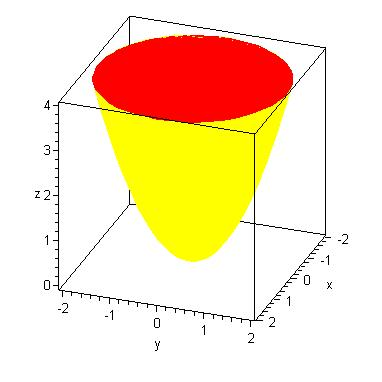
\includegraphics[height=\myheight]{10-SurfaceTripleIntegrals/support/triple-1}
\end{wrapfigure}
The region above the paraboloid $z=x^2+y^2$ below the plane $z=4$ has
$x$ values between $-2$ and $2$ (the outer bounds). The $y$ values lie
in the cylinder $x^2+y^2=4$ or $y=-\sqrt{4-x^2}$ and $y=\sqrt{4-x^2}$.
The $z$ values lie between the surfaces $z=x^2+y^2$ and $z=4$.  So we
have for our bounds the inequalities $-2\leq x\leq 2$, $-\sqrt{4-x^2}\leq y\leq
\sqrt{4-x^2}$, and $x^2+y^2\leq z\leq 4$ (planes, cylinders, surfaces) which
can be used to find the volume of this region by the triple integral
$V=\int_{-2}^{2}\int_{-\sqrt{4-x^2}}^{\sqrt{4-x^2}}\int_{x^2+y^2}^{4}1 dz dy
dx$. This integral is rather complicated to solve by hand as written,
but using an appropriate high dimensional change of coordinates, this
integral becomes rather trivial.  Spend most of your time learning to
set up integrals rather than solving them.

\begin{wrapfigure}[6]{l}[24pt]{0pt}
\newcommand{\myheight}{.8in}
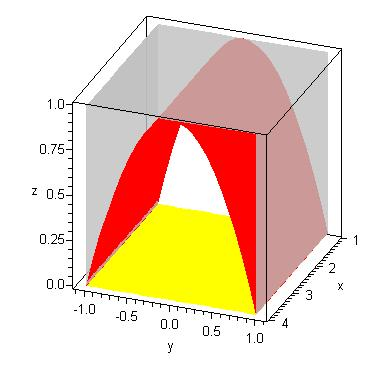
\includegraphics[height=\myheight]{10-SurfaceTripleIntegrals/support/triple-2}
\end{wrapfigure}
The region $D$ below the cylinder $z=1-y^2$ above the $xy$ plane and
between the planes $x=1,x=4$ can be found as follows.  If we choose
$x,y,z$, as our outer, middle, inner bounds, then $1\leq x\leq 4,-1\leq y\leq 1,0\leq
z\leq 1-y^2$.  If we choose instead the order $z,x,y$, then we have $0\leq
z\leq 1$, $1\leq x\leq 4$, and $-\sqrt{1-z}\leq y\leq \sqrt{1-z}$ (just solve for $y$
in the equation $z=1-y^2$ to find the bounds for $y$).  Hence the
volume of this region can be written two ways as
$V=\int_{1}^{4}\int_{-1}^{1}\int_{0}^{1-y^2}1 dz dy dx =
\int_{0}^{1}\int_{-1}^{1}\int_{-\sqrt{1-z}}^{\sqrt{1-z}}1 dy dx dz$. 

We currently have two ways of finding volume, either $\iint_R fdA$ or
$\iiint_D 1 dV$.  Using differential notation $dA=fdx=dxdy$ and $dV =
fdA = fdxdy = dxdydz$ helps remind us of how to find area and volume
in any manner.  The formula $dA=fdx$ reminds us that little pieces of
area can be found by taking a height times a little change in $x$ and
using a single integral.  The formula $dA = dxdy$ reminds us that area
can also be found using a double integral as area is little changes in
width times little changes in length.  Similarly $dV=fdA=fdxdy$
reminds us that volume can be found using a double integral, or
$dV=dxdydz$ says that volume can be found using a triple integral.
The shell method $dV=2\pi xf(x)dx$ and disk method $dV = \pi (f(x))^2dx$
can also be summarized in differential notation, and since there is
only $dx$ you only use a single integral.  If you can remember how to
compute a little piece of volume $dV$ using any of these formulas,
then total volume is found by adding up all the little pieces. The
number of integrals used depends on the number of differentials like
$dx$, $dy$, or $dz$. If you use a single integral sign to represent
however many iterated integrals you need (depending on the
differential), then you can write area as ``add up little bits of
area'' ($A=\int_RdA$), and volume as ``add up little bits of volume''
($V=\int_D dV$), where the number of integrals is determined by the
differential formula you choose for $dA$ or $dV$.

\subsection{Changing Coordinate Systems: Generalized substitution}
\prepproblems{14.7: 13, 19\\14.8: 27}%
Just as we did with polar coordinates in two dimensions, we can
compute a Jacobian for any change of coordinates in three dimensions.
We will focus on cylindrical and spherical coordinate systems.
Remember that the Jacobian of a transformation is the absolute value
of the determinant of the derivative of the transformation.

\subsubsection{Cylindrical Coordinates}
Cylindrical coordinates are defined by $x=r\cos\theta$, $y=r\sin\theta$, and
$z=z$, which we can represent using function notation as
$T(r,\theta,z)=\langle r\cos\theta, r\sin\theta,z\rangle$. The derivative of this transformation
is 
$DT(r,\theta,z)= 
\begin{bmatrix}
\cos\theta&-r\sin\theta&0\\
\sin\theta&r\cos\theta&0\\
0&0&1
\end{bmatrix}$. The Jacobian of the transformation is
$\frac{\partial(x,y,z)}{\partial(r,\theta,z)} = |\det(DT(r,\theta,z))| = |r|$. Provided that
$r\geq 0$, we have the differential formula $dV=rdrd\theta dz$, or in integral
form the equation $\iiint_{D_{xyz}} f(x,y,z)dxdydz = \iiint_{D_{r\theta z}}
f(T(r,\theta,z))\frac{\partial(x,y,z)}{\partial(r,\theta,z)}drd\theta dz=  \iiint_{D_{r\theta z}}
f(T(r,\theta,z))(r)drd\theta dz $. In summary, converting to cylindrical
coordinates requires that we multiply by $r$. Cylindrical coordinates
are extremely useful for problems which involve cylinders,
paraboloids, and cones. 

\begin{wrapfigure}[6]{l}[24pt]{0pt}
\newcommand{\myheight}{.8in}
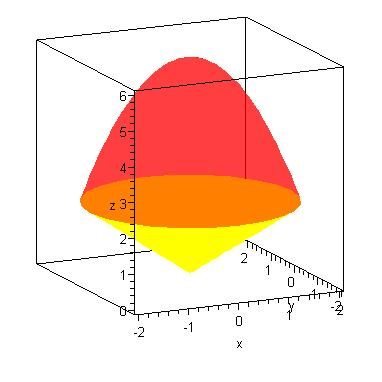
\includegraphics[height=\myheight]{10-SurfaceTripleIntegrals/support/cylindrical-1}
\end{wrapfigure}
We now find the volume of the region $D$ in space which is above the
cone $z=\sqrt{x^2+y^2}$ and below the paraboloid $z=6-x^2-y^2$.
Switching to cylindrical coordinates, these equations become $z=r$ for
the cone and $z=6-r^2$ for the paraboloid.  The surfaces intersect
when $r=6-r^2$, or $r^2+r-6 = (r+3)(r-2)=0$, or $r=2,-3$. Since $z>0$,
we know that the intersection we seek is at $r=2$. So the region $D$
in space is the set of points above $z=r$, below $z=6-r^2$, and inside
the cylinder $r=2$.  We can describe this region using the
inequalities $0\leq \theta\leq 2\pi$, $0\leq r\leq 2$, and $r\leq z\leq 6-r^2$. This gives us
the volume as $V = \int_0^{2\pi}\int_0^2\int_r^{6-r^2}(r)dzdrd\theta$. 

\begin{wrapfigure}[6]{l}[24pt]{0pt}
\newcommand{\myheight}{.8in}
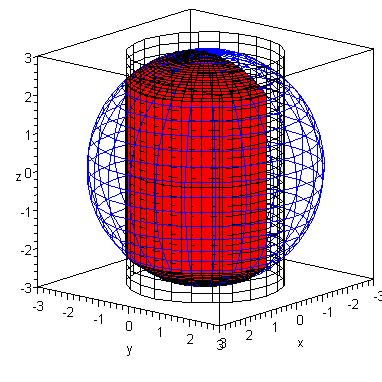
\includegraphics[height=\myheight]{10-SurfaceTripleIntegrals/support/cylindrical-2}
\end{wrapfigure}
The integral
$\int_0^2\int_{-\sqrt{4-x^2}}^{\sqrt{4-x^2}}\int_{-\sqrt{9-x^2-y^2}}^{\sqrt{9-x^2-y^2}}dzdydx$
represents the volume of the region in space satisfying the
inequalities $0\leq x\leq 2$, ${-\sqrt{4-x^2}}\leq y\leq {\sqrt{4-x^2}}$, and
${-\sqrt{9-x^2-y^2}}\leq z\leq{\sqrt{9-x^2-y^2}}$, or the region in space
with positive $x$ values inside the cylinder $x^2+y^2=4$ and inside
the sphere $x^2+y^2+z^2=9$. Since this problem involves a cylinder, we
will write the integral in cylindrical coordinates.  The region is
described using $-\pi/2\leq \theta\leq \pi/2$, $0\leq r\leq 2$, and $-\sqrt{9-r^2}\leq z\leq 
\sqrt{9-r^2}$, which means that we can rewrite the integral as $V=
\int_{-\pi/2}^{\pi/2}\int_0^2\int_{-\sqrt{9-r^2}}^{\sqrt{9-r^2}}(r)dzdrd\theta $. The
volume of the region outside the cylinder of radius 2, inside the
sphere of radius 3, with positive $x$ values is given by either $V=
\int_{-\pi/2}^{\pi/2}\int_2^3\int_{-\sqrt{9-r^2}}^{\sqrt{9-r^2}}(r)dzdrd\theta $ or $V=
\int_{-\pi/2}^{\pi/2}\int_{-\sqrt 5}^{\sqrt{5}}\int_{2}^{\sqrt{9-z^2}}(r)drdzd\theta $
(since the cylinder intersects the sphere at a height of $\sqrt 5$).



\subsubsection{Spherical Coordinates}
Spherical coordinates are defined by $T(\rho,\theta,\phi) = \langle\rho\cos\theta\sin\phi,
\rho\sin\theta\sin\phi,\rho\cos\phi\rangle$.  The Jacobian of this transformation is $\ds
\frac{\partial(x,y,z)}{\partial(\rho,\theta,\phi)} = |\det(DT(\rho,\theta,\phi)| = |-\rho^2\sin\phi|$ (verify
this as homework). Using differential notation, we write
$dV=dxdydz=|\rho^2\sin\phi|d\rho d\theta d\phi$, so that whenever you convert to
spherical coordinates from rectangular, you have to multiply by
$|\rho^2\sin\phi|$ inside the integral, or just $\rho^2\sin\phi$ if you require
{$0\leq \phi\leq \pi$}. Problems which involve cones and spheres often have
simple integrals in spherical coordinates.

The volume inside a sphere of radius $a$ is
$\int_{-a}^{a}\int_{-\sqrt{a^2-x^2}}^{\sqrt{a^2-x^2}}\int_{-\sqrt{a^2-x^2-y^2}}^{\sqrt{a^2-x^2-y^2}}dzdydx$.
This integral is rather difficult to solve by hand (if it is even
possible).  However the region inside the sphere is describe in
spherical coordinates as $0\leq \phi \leq \pi$, $0\leq \theta\leq 2\pi$, and $0\leq \rho\leq a$.  Hence
the volume is found using $V=\int_0^\pi\int_0^{2\pi}\int_0^a \rho^2\sin\phi d\rho d\theta d\phi$.
This integral can be evaluated using elementary techniques and gives
the volume $V=\frac{4}{3}\pi a^3$.


\begin{wrapfigure}[5]{l}[24pt]{0pt}
\newcommand{\myheight}{.8in}
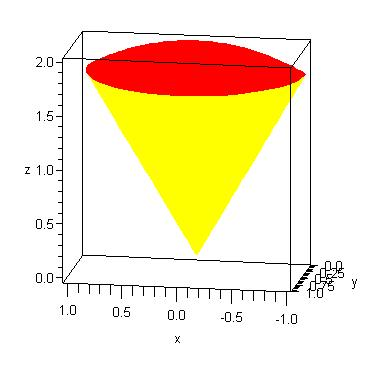
\includegraphics[height=\myheight]{10-SurfaceTripleIntegrals/support/spherical-1}
\end{wrapfigure}
The integral $\int_{0}^{\pi}\int_{0}^{1}\int_{\sqrt{3}r}^{\sqrt{4-r^2}}rdzdrd\theta$
represents the region in space with $y\geq 0$, $r\leq 1$, above the cone
$z=\sqrt 3 r$, and below the sphere $z^2=4-r^2$. The cone and sphere
intersect precisely when $r=1$.  In rectangular coordinates, the
integral is
$\int_{-1}^{1}\int_{0}^{\sqrt{1-x^2}}\int_{\sqrt{3(x^2+y^2)}}^{\sqrt{4-x^2-y^2}}dzdydx$. 
In spherical coordinates, the cone is given by the equation $\phi=\pi/6$
(draw a right triangle with hypotenuse 2 and one side length 1), and
the sphere is given by the equation $\rho = 2$. The integral becomes
$\int_{0}^{\pi}\int_{0}^{\pi/6}\int_{0}^{2}\rho^2\sin\phi d\rho d\phi d\theta$. 









\subsection{Physical Applications}
\prepproblems{14.6: 33, 49, 63\\ 14.7: 21, 35}%
Integrals are used in a wide variety of applications.  Notice that in
all of the applications we have done this semester, a formula which
works for double integrals will also work for single, line, surface,
and triple integrals.  The differentials $dx,ds,dA,d\sigma, dV$ remind us
which dimension we are working in.  For lack of a better notation,  I
will use $d\square$ to represent any of these differentials when you
are free to pick the needed differential. The line integrals section
contains the details for each of the physical quantities we compute.


\subsubsection{The Short Version}
Everything we learned about physical applications this semester can be
summarized in the following table list, where recall that $d\square$
stands for any of $dx,ds,dA,d\sigma,dV$.
\begin{itemize}
\item Area: $dA = fdx,fds, dxdy, rdrd\theta, \frac{\partial(x,y)}{\partial(u,v)}dudv$, 
\item Volume: $dV = fdA,dxdydz, rdrd\theta dz, \rho^2\sin\phi d\rho d\theta d\phi,
\frac{\partial(x,y,z)}{\partial(u,v,w)}dudvdw$, 
\item Surface Area: $d\sigma = |\vec r_u\times \vec r_v|dudv =
\sqrt{f_x^2+f_y^2+1}dxdy$
\item Average Value: $\bar f\square = \int fd\square$, and $dm = \delta
d\square , \delta dx, \delta ds, \delta dA, \delta d\sigma, \delta dV $
\item Center of Mass: $(\bar x,\bar y,\bar z)m = \int(x,y,z) dm$, where
$\int \bar x dm = \int x dm$ is a first moment of mass
\item Moment of Inertia: $I = \int rad^2 dm$ is a moment of inertia, and
$\int R^2 dm = \int r^2 dm$ gives $R^2 m =I$ or $R=\sqrt{I/m}$. Recall that
$rad^2 = y^2+z^2$ for $I_x$, $rad^2=x^2+z^2$ for $I_y$, and
$rad^2=x^2+y^2$ for $I_z$.
%\item Flux: $d\text{Flux} = \vec F\cdot \vec n d\sigma $ or $ \vec F\cdot \vec n
%ds$ where $\vec n$ is a normal vector to either a surface $S$ or a
%curve $C$.
%\item Circulation: $d\text{Circ} = \vec F\cdot \vec T ds  = Mdx+Ndy$.
\end{itemize}
I strongly suggest that as you do each problem, start from a formula
in differential notation, and then modify it so that you have the
right number of integrals.  If you do this, you will learn how to do
calculus in all dimensions with ease. 

\begin{example}
  Consider the region in space inside the cylinder $r=4$ bounded above
  by the cone $z=r$ and below by the $xy$-plane.  Using cylindrical
  coordinates, we have $dV = rdzdrd\theta$. The volume is
  $\int_{0}^{2\pi}\int_0^4\int_0^r rdzdrd\theta$.  If the density is
  $\delta(x,y,z) =x^2+z$, then we have
  \begin{align*}
    \bar y &= \frac{\int y dm}{\int dm}= \frac{\iiint_D y \delta
      dV}{\iiint_D \delta dV}= \frac{\int_{0}^{2\pi}\int_0^4\int_0^r
      r\sin\theta((r\cos\theta)^2+z)rdzdrd\theta}
    {\int_{0}^{2\pi}\int_0^4\int_0^r ((r\cos\theta)^2+z) rdzdrd\theta}\\
    R_z &= \sqrt{\frac{\int r^2 dm}{\int dm}} =\sqrt{\frac{\int
        x^2+y^2 dm}{\int dm}} = \sqrt{\frac
      {\int_{0}^{2\pi}\int_0^4\int_0^r((r\cos\theta)^2+(r\sin\theta)^2)
        ((r\cos\theta)^2+z) rdzdrd\theta}
      {\int_{0}^{2\pi}\int_0^4\int_0^r ((r\cos\theta)^2+z)
        rdzdrd\theta}}
  \end{align*}
\end{example}

\begin{example}
  The temperature at each point in space of a solid covering the
  region {$D$} (the upper portion of the sphere of radius 4 centered
  at the origin) is given by $T(x,y,z) = \sin(xy+z)$.  The volume and
  average temperature are

\begin{align*}
  V&=\int_{-4}^{4} \int_{-\sqrt{16-x^2}}^{\sqrt{16-x^2}}
  \int_{0}^{\sqrt{16-x^2-y^2}} dz dy dx\\
  AV&=\frac{1}{V}\int_{-4}^{4} \int_{-\sqrt{16-x^2}}^{\sqrt{16-x^2}}
  \int_{0}^{\sqrt{16-x^2-y^2}} \sin(xy+z) dz dy dx.
\end{align*}
\end{example}





%%% Local Variables: 
%%% mode: latex
%%% TeX-master: "../multivariable-calculus"
%%% End: 






\newgeometry{left=1in,right=1in,top=1in,bottom=1in}
\newpage

\section{Preparation}

\subsection{Lesson Plans}

This chapter covers the following ideas. When you create your lesson plan, it should contain examples which illustrate these key ideas. Before you take the quiz on this unit, meet with another student out of class and teach each other from the examples on your lesson plan. 

% A list of objectives for the chapter
%\begin{enumerate}
%\item ...
%\end{enumerate}


\begin{enumerate}
\item Explain how to setup surface integrals, as well as how to
compute surface area.
\item Explain how to set up and compute triple
  integrals, as well as how to interchange the bounds of
  integration. Use these ideas to find volume.
\item For surfaces and solid regions, find area,
  mass, centroids, center of mass, moments of interia, and radii of
  gyration.
\item Explain how to change coordinate systems in integration, in
  particular to polar, cylindrical, and spherical coordinates. Explain
  what the Jacobian of a transformation is and how to use it.
\end{enumerate}

%%% Local Variables: 
%%% mode: latex
%%% TeX-master: "../multivariable-calculus"
%%% End: 
%$


%\subsection{Preparation Problems}

%Here are the preparation problems for this unit.

\subsection{Homework}

In the following list, the ``basic practice'' problems should be quick
problems to help you master the ideas.  The ``good problems'' will
require a little more work.  The theory and application problems are
ones that will challenge you more; make sure you do the problems from
this area to fully master the material.  

{\centering
\begin{tabular}{lcllll}\toprule
Topic &Sec &Basic Practice &Good Problems &Thy/App \\\midrule

Surface area & 14.5 & 1--24 & 27--34 & 37--41\\\hline
Parametric surfaces & 15.5 & 1--4, 35--42 & 13--26\\\hline
Surface integrals & 15.6 & 1--22 & 37--40\\\bottomrule
Triple integrals & 14.6 & 1--38, 63--66 & 43--58 & 39-40, 61--62, 67--70\\\hline
Spherical and Cylindrical & 14.7 & 1--22 & 23--38 & 43--46\\\hline
Jacobians & 14.8 & 27--30&&\\\hline
\end{tabular}

} 
\bigskip
It is crucial that you do not attempt to solve every integral.  For
the most part, you are learning to set up integrals in high
dimensions. You should do many more than 5 problems a day if you want
to become proficient at multiple integration.  \textbf{I would suggest
  that you do at least 15 or more problems a day in the assigned
  sections}, where you spend time setting up integrals and not solving
them.


%%% Local Variables: 
%%% mode: latex
%%% TeX-master: "../multivariable-calculus"
%%% End: 


%%% Local Variables: 
%%% mode: latex
%%% TeX-master: "../multivariable-calculus"
%%% End: 

\restoregeometry


%\backmatter

%\printindex








%\appendix
%
%\chapter{The First Appendix}
%
%The \verb"\appendix" command should be used only once. Subsequent appendices can
%be created using the Chapter command.
%
%\chapter{The Second Appendix}
%
%Some text for the second Appendix.
%
%This text is a sample for a short bibliography. You can cite a book by making use of
%the command \verb"\cite{KarelRektorys}": \cite{KarelRektorys}. Papers can be cited
%similarly: \cite{Bertoti97}. If you want multiple citations to appear in a single set
%of square brackets you must type all of the citation keys inside a single citation,
%separating each with a comma. Here is an example: \cite{Bertoti97, Szeidl2001,
%Carlson67}.
%
%\begin{thebibliography}{9}
%\bibitem {KarelRektorys}Rektorys, K., \textit{Variational methods in Mathematics,
%Science and Engineering}, D. Reidel Publishing Company,
%Dordrecht-Hollanf/Boston-U.S.A., 2th edition, 1975
%
%\bibitem {Bertoti97} \textsc{Bert\'{o}ti, E.}:\ \textit{On mixed variational formulation
%of linear elasticity using nonsymmetric stresses and displacements}, International
%Journal for Numerical Methods in Engineering., \textbf{42}, (1997), 561-578.
%
%\bibitem {Szeidl2001} \textsc{Szeidl, G.}:\ \textit{Boundary integral equations for
%plane problems in terms of stress functions of order one}, Journal of Computational and
%Applied Mechanics, \textbf{2}(2), (2001), 237-261.
%
%\bibitem {Carlson67}  \textsc{Carlson D. E.}:\ \textit{On G\"{u}nther's stress functions
%for couple stresses}, Quart. Appl. Math., \textbf{25}, (1967), 139-146.
%\end{thebibliography}
%


%\backmatter

%
%\chapter{Afterword}
%
%The back matter often includes one or more of an index, an afterword,
%acknowledgements, a bibliography, a colophon, or any other similar item. In
%the back matter, chapters do not produce a chapter number, but they are
%entered in the table of contents. If you are not using anything in the back
%matter, you can delete the back matter TeX field and everything that follows it.
\end{document}


%%% Local Variables: 
%%% mode: latex
%%% TeX-master: t
%%% End: 
